%% plantmodel v2 -- SMP&T submission
%% Assembled from paper/v2/sections/*.tex.  Compile with:
%%   pdflatex main && bibtex main && pdflatex main && pdflatex main
\documentclass[a4paper,fleqn]{cas-sc}

\usepackage[numbers]{natbib}
\usepackage{amsmath,amssymb}
\usepackage{booktabs}
\usepackage{graphicx}
\usepackage{url}
\usepackage{siunitx}

%% figs/ first: v2 owns its own figure set and must not silently fall back to
%% the v1 directory, which holds superseded versions of several file names.
\graphicspath{{figs/}}

\begin{document}

\let\WriteBookmarks\relax
\def\floatpagepagefraction{1}
\def\textpagefraction{.001}

\shorttitle{Runtime supply--demand closure in a diel plant growth model}
\shortauthors{TODO(AUTHOR)}

\title[mode=title]{Closing stomatal supply against photosynthetic demand at
runtime: a verified diel plant growth model and the boundary of its validity}

%% TODO(AUTHOR): author names, affiliations, e-mail addresses and the
%% corresponding-author mark.  Left as placeholders deliberately -- these are
%% not ours to invent.
\author[1]{TODO(AUTHOR) Given Name Surname}
\ead{TODO(AUTHOR) email@institution}
\affiliation[1]{organization={TODO(AUTHOR) Institution},
                addressline={TODO(AUTHOR) Address},
                city={TODO(AUTHOR) City},
                country={TODO(AUTHOR) Country}}

\begin{abstract}
Mechanistic models of plant growth usually prescribe carbon input or compute it
from a photosynthesis routine that is solved separately from stomatal
conductance. This work reports a modular simulation model in which the supply
and demand sides of leaf gas exchange are closed against each other at every
evaluation: a Jarvis conductance and a Farquhar assimilation function are
combined into a quadratic in the intercellular CO$_2$ concentration and solved
in closed form, replacing a fixed-point iteration that we show admits a
period-two orbit under water stress. Around this closure the model integrates
eleven states covering starch, sucrose and vacuolar sugar, nitrogen and
phosphorus acquisition with explicit costs, and leaf and root biomass. Carbon
conservation over the carbohydrate subsystem closes to machine precision.
Rather than fitting coefficients per experimental condition, we hold a single
parameter set across four photoperiods and report what that costs: relative
growth rate is reproduced with a mean absolute percentage error of 8.58~\% and a
worst case of 11.75~\%, against a published baseline whose apparent agreement is
a bisection residual of eight coefficients fitted to eight observations.
Leave-one-photoperiod-out cross-validation gives a held-out error of 13.18~\%
for a photoperiod-independent growth coefficient and 4.36~\% when the
coefficient is allowed a linear photoperiod dependence. Diel starch is
reproduced in both shape and level; sucrose is reproduced in shape but is a
factor two to three low in absolute concentration, which we report rather than
absorb. Ablation shows that computing the carbon input, rather than prescribing
it, is what carries the photoperiod response. Variance-based sensitivity
analysis places 96~\% of output variance in parameter interactions rather than
main effects. Finally we locate the boundary of the model's validity: the diel
carbon balance closes only up to a 15~h photoperiod, and beyond it starch
accumulates without bound, a limitation we characterise rather than conceal.
\end{abstract}

\begin{keywords}
plant growth simulation \sep
diel carbohydrate turnover \sep
Farquhar--Jarvis coupling \sep
verification and validation \sep
variance-based sensitivity analysis \sep
out-of-sample cross-validation
\end{keywords}

\maketitle

\section{Introduction}
\label{sec:intro}

\textit{Arabidopsis thaliana} grows in a light environment that switches off
every day. During the light phase the plant assimilates carbon and stores part
of it as transient leaf starch. During the night this reserve is the only carbon
source for respiration, maintenance and growth. Measurements show that the
reserve is degraded at an almost constant rate and is nearly exhausted at dawn
\cite{Graf2010,Smith2007}. The plant therefore behaves as if it rations a known
amount of carbon over a night of known length \cite{Scialdone2013}. When the
photoperiod changes, both the amount and the length change together, and the
rationing problem changes with them \cite{Sulpice2014,Stitt2012}. This makes
photoperiod a useful test case for a simulation model, because a single
environmental variable moves the light-phase carbon gain and the dark-phase
reserve use at the same time.

The problem is difficult to simulate because it couples processes on very
different time scales. Stomatal opening and leaf assimilation respond within
minutes to light, temperature and humidity. Starch and sucrose pools turn over
within hours. Nutrient status changes over days and biomass accumulates over
weeks. The carbon available for growth at any instant is not a property of any
single equation. It is the result of the environment, the gas-exchange
machinery and the internal carbohydrate and nutrient state acting together
\cite{Farquhar1980,ThornleyJohnson1990}. A model that describes only
photosynthesis, or only biomass accumulation, cannot represent this. For a
simulation study the main task is therefore to build a stable numerical
workflow in which these subsystems exchange fluxes consistently over the
day--night cycle.

Existing models resolve parts of this chain, but usually not the whole chain at
the resolution the problem needs. Crop and field-scale simulators such as
WOFOST, APSIM and DSSAT integrate growth, water and nitrogen over seasons
\cite{deWit2019,Holzworth2014,Jones2003}. For robustness and runtime they
obtain the carbon input from a light-use-efficiency term, a radiation-use
coefficient or a look-up table, and they usually advance the state on a daily
step. Soil--plant transport models and functional--structural plant models add
detail in other directions, in water transport and in architecture
respectively \cite{Janott2011,DeReffye2020,Louarn2020}. At the other end of
the scale range, leaf gas-exchange models resolve the process that the crop
models prescribe. The Farquhar--von Caemmerer--Berry biochemical model and
Jarvis-type or optimality-based stomatal formulations describe assimilation and
conductance in detail \cite{Farquhar1980,Jarvis1976,Ball1987,Medlyn2011}, and
the coupling between them has been studied extensively
\cite{Damour2010,Buckley2017}. These models are formulated and tested as
steady-state algebraic systems at a fixed carbohydrate status, so they stop at
the leaf. Few published models compute the supply--demand operating point at
every step and then carry that carbon input through a diel starch and sucrose
economy into biomass.

This paper presents such a model and reports its evaluation. The model is a
whole-plant dynamic simulator with eleven state variables, organised as six
submodels with declared inputs, outputs and parameters
(Figure~\ref{fig:overview}). S1 maps clock time to
the environmental drivers. S2 computes stomatal conductance from a
multiplicative Jarvis formulation, which acts as the supply side of gas
exchange. S3 computes net assimilation as a function of intercellular CO$_2$
from the Farquhar C3 biochemistry, which acts as the demand side. S4 closes
supply against demand. S5 holds the diel carbohydrate economy, the starch and
sucrose pools and the nitrogen and phosphorus uptake and costs. S6 converts
sucrose into leaf and root biomass. Submodels S2--S4 form a fast algebraic
subsystem, and S5--S6 form the slow differential subsystem that is integrated
in time.

The methodological content of the work sits in four places, and this is what we
expect to transfer to other coupled biophysical simulators. First, the
gas-exchange operating point is solved algebraically at runtime. Substituting
Fick's law into the branch-wise Farquhar expression gives a quadratic equation
in the intercellular CO$_2$ concentration. This quadratic is solved branch by
branch, with an explicit admissibility rule for the roots. No inner iteration
is then required inside the derivative evaluation. Second, the fast/slow decomposition
is explicit: the algebraic subsystem is eliminated exactly inside each
derivative call, so the remaining differential system is integrated with an
explicit adaptive method. Third, the implementation is verified before it is
compared with data. The checks are the residual of the algebraic closure, an
integration refinement study, and a bookkeeping check on the starch and sucrose
subsystem.
Fourth, model behaviour is analysed with a screening step followed by a
variance-based global sensitivity analysis over declared parameter ranges.

The evaluation design is chosen so that calibration and prediction stay
separate. Four coefficients are fitted and shared across all photoperiods,
where the earlier version of this model used eight coefficients fitted
separately for each photoperiod. Predictive accuracy is then measured by
holding out whole photoperiods, that is, by fitting on three light regimes and
predicting the fourth. Under this design the model reaches a held-out mean
absolute percentage error of 4.36\,\% in relative growth rate
(Figure~\ref{fig:crossval}). This value applies when one growth coefficient is
allowed to depend linearly on photoperiod. We also measure the
range of photoperiods over which the model remains usable, and we report the
boundary of that range together with the mechanism that breaks first.

The contributions of the paper are the following.
\begin{enumerate}
\item A coupled whole-plant simulation model in which Jarvis stomatal
  conductance and Farquhar C3 photosynthesis produce the carbon input at every
  step, and that input is propagated through diel starch and sucrose dynamics,
  nutrient uptake and costs, and biomass growth (Section~\ref{sec:model}).
\item An analytic runtime solution of the supply--demand closure as a quadratic
  in the intercellular CO$_2$ concentration, embedded in a fast/slow numerical
  workflow (Sections~\ref{sec:model} and~\ref{sec:implementation}).
\item A verification protocol for the implementation that is independent of any
  comparison with data, covering the algebraic closure, the time integration
  and the carbohydrate bookkeeping (Section~\ref{sec:implementation}).
\item An evaluation with four shared fitted parameters instead of a
  per-photoperiod calibration. The design uses leave-one-photoperiod-out
  cross-validation, an ablation of the carbon-input pathway, and a global
  sensitivity analysis over declared ranges
  (Sections~\ref{sec:protocol} and~\ref{sec:results}).
\item A measured validity envelope. We report the photoperiod range in which
  the diel starch balance closes, the photoperiod at which it stops closing,
  and the bound on the simulated growth response to day length
  (Sections~\ref{sec:results} and~\ref{sec:limitations}).
\end{enumerate}

The rest of the paper is organised as follows.
Section~\ref{sec:related} reviews mechanistic growth models, gas-exchange
formulations, diel carbohydrate modelling and simulation evaluation practice,
and states the gap that this work addresses. Section~\ref{sec:model} gives the
model formulation as six submodels with their states, inputs and parameters.
Section~\ref{sec:implementation} describes the numerical implementation and the
verification results. Section~\ref{sec:protocol} defines the photoperiod
scenarios, the calibration and cross-validation design, the ablation variants
and the sensitivity protocol. Section~\ref{sec:results} reports the results,
Section~\ref{sec:discussion} interprets them, Section~\ref{sec:limitations}
states what cannot be concluded, and Section~\ref{sec:conclusion} concludes.

% ============================================================
\section{Related Work}
\label{sec:related}

This section positions the model against four bodies of work. These are
mechanistic whole-plant and crop simulation, leaf gas-exchange modelling, diel
carbohydrate turnover in \textit{Arabidopsis thaliana}, and evaluation practice
in simulation studies. The aim is to locate the contribution, not to survey
each field completely.

\subsection{Mechanistic plant growth simulation models}

Mechanistic growth models link physiological processes, microclimate and
biomass change over time. The spatial and temporal scale of a model decides
where it can be applied. Spatially, models cover the leaf, the organ, the whole
plant, the canopy or the field. Temporally, they range from minutes, for
gas exchange, through hours and days, for carbon allocation, to whole seasons,
for yield. Crop simulation platforms such as APSIM, DSSAT and WOFOST are mature
tools for growth, water and nitrogen dynamics at field scale
\cite{Holzworth2014,Jones2003,deWit2019}. Recent process-based systems extend
this to detailed agronomic management and are validated against field data
\cite{BuckleyPaules2025}. Comparative studies indicate that process-based
formulations follow seasonal variation in climate better than purely empirical
ones \cite{Mamassi2024}.

Several other model families address different aspects of the same problem.
Functional--structural plant models combine architecture with physiological
modules, and they show how spatial structure and dynamic growth can be
integrated \cite{Louarn2020,Sievnen2014,DeReffye2020}. Soil--plant water
transport models describe flow from the soil through the xylem, and a
one-dimensional formulation can be as effective as a three-dimensional one at
much lower computational cost \cite{Janott2011}. Discrete approaches based on
the discrete element method are used for root--soil contact problems
\cite{Tian2024}. Optimality and energy-budget models assume that allocation
maximises a criterion such as growth or resource-use efficiency
\cite{Russo2022}. Continuous formulations describe biomass, water or vegetation
dynamics as systems of differential equations and allow formal analysis
\cite{Meron2019,ThornleyJohnson1990}. Source--sink descriptions of carbon
partitioning between shoot and root belong to the same tradition
\cite{Marcelis1996,Feller2015,Thornley1972}.

Two properties of this literature matter here. Modular organisation is common
and useful, because it lets each component be tested on its own
\cite{Sievnen2014,Zeigler2000}. The carbon input, however, is often prescribed
rather than computed. Light-use-efficiency terms, radiation-use coefficients
and look-up tables are standard in field-scale simulators, and daily time steps
are common \cite{Jones2003,deWit2019,Holzworth2014}. This separates the carbon
source from the environment and from the internal state of the plant. The model
then cannot represent the feedback between stomatal behaviour, intercellular
CO$_2$, carbohydrate status and growth.

\subsection{Photosynthesis and stomatal conductance modelling}

Photosynthesis sets the primary carbon input, so its description controls
everything downstream. For C3 plants the standard biochemical model is the
Farquhar--von Caemmerer--Berry formulation, which relates net assimilation to
intercellular CO$_2$ through Rubisco-limited carboxylation and RuBP
regeneration \cite{Farquhar1980,vonCaemmerer2000}. Its parameters, mainly
$V_{cmax}$, $J$, $\Gamma^*$, $K_c$, $K_o$ and $R_d$, and their temperature
dependence are well documented \cite{Sharkey2007,Bernacchi2001,Dubois2007}.

Assimilation also depends on the diffusive supply of CO$_2$, which stomatal
conductance controls \cite{Lawson2014}. Stomatal models therefore connect
microclimate to carbon gain. The main formulations are the empirical
multiplicative Jarvis model, the Ball--Berry family and the Medlyn optimality
model \cite{Jarvis1976,Ball1987,Medlyn2011}. The Jarvis form expresses
conductance as a product of response functions to irradiance, vapour-pressure
deficit, temperature, CO$_2$ and plant water status \cite{Jarvis1976,YU2017,Yu2021}.
It is convenient in a simulation setting because time-varying drivers from a
scenario or from measurements enter it directly. Reviews of coupled
formulations compare these alternatives and discuss where each is appropriate
\cite{Damour2010,Buckley2017}.

Coupling the two sides introduces a feedback. Intercellular CO$_2$ sets the
assimilation rate in the biochemical model, while conductance sets how much
CO$_2$ can diffuse into the leaf. The operating point is therefore defined
implicitly and must be found at every evaluation of the model
\cite{Damour2010}. Iterative solutions are widely used, and analytic solutions
of the coupled system for particular stomatal formulations are also known
\cite{Buckley2017,Kim2003}. The Farquhar and Jarvis equations used here are
inherited physiological components, not a contribution of this paper. The
contribution is the way they are solved at runtime and coupled to the
carbohydrate, nutrient and biomass states.

\subsection{Diel carbohydrate turnover and photoperiod}

Carbohydrate dynamics are the link between assimilation and growth. In the
light phase, assimilated carbon is partitioned between mobile sugars, mainly
sucrose, and transient reserves, mainly leaf starch. In the dark phase, starch
degradation supplies carbon for respiration, maintenance and growth
\cite{Stitt2012,Smith2007}. In \textit{Arabidopsis thaliana} this degradation
is closely regulated, and the reserve is almost completely used by dawn
\cite{Graf2010,Scialdone2013,Webb2015}. Mathematical models of the process
connect circadian regulation, sucrose availability and sugar signalling to
carbon partitioning and growth \cite{Feugier2013,Seki2017}. Sucrose transport
and the separation between cytosolic and vacuolar sucrose have also been
described in detail \cite{Lohaus2000,Nadwodnik2008}.

Photoperiod changes the balance between daytime accumulation and nocturnal
consumption. A short day limits the time available for assimilation and
lengthens the interval in which growth depends on stored starch. A long day
extends direct carbon input and shortens the interval of reserve use.
Experiments over contrasting short and long photoperiods show that
\textit{Arabidopsis thaliana} adjusts partitioning and growth to day length
\cite{Sulpice2014,Mengin2017,Annunziata2017}. This makes photoperiod scenarios
a suitable evaluation setting: they perturb both phases of the diel carbon
economy through one variable, and they have documented growth and carbohydrate
responses.

Growth also depends on nutrient status. Nitrogen and phosphorus affect
photosynthetic capacity, metabolism and allocation, and mechanistic models
introduce them as internal states or as limiting factors
\cite{Gastal2002,Xu2012,Barber1995,Shen2011,Carstensen2018}. Models that
resolve the diel cycle in detail, however, usually treat assimilation as given
\cite{Scialdone2013,Graf2010,Feugier2013}. The day--night carbohydrate balance
and the gas exchange that produces it are then not solved as one system.

\subsection{Verification, validation and sensitivity practice in simulation}

Evaluation of plant models normally compares simulated and reference values for
biomass, relative growth rate, and water or nutrient fluxes
\cite{Wallach2018,Holzworth2014,Jones2003}. Two distinctions from simulation
methodology are relevant here. The first is between verification and
validation: agreement with measurements does not show that the numerical
procedures inside the simulator are correct \cite{Zeigler2000,Cellier1991}.
Residual checks against analytic solutions, integration refinement studies and
conservation or bookkeeping checks address a different question from data
agreement. The second is between calibration residual and predictive error.
When a model is fitted and evaluated against the same small set of aggregate
observations, the reported error is a calibration residual. Multi-model studies
of crop simulators show how strongly reported accuracy depends on the
calibration protocol \cite{Maiorano2017,Wallach2018}.

Ablation is a further tool for attributing behaviour to model structure. It
compares variants in which a component is removed, simplified or replaced.
For a coupled model of the kind studied here, three variants are informative.
The first uses a prescribed carbon input. The second computes assimilation at
fixed conductance. The third is the full variant with environment-responsive
conductance. Such a comparison separates the effect of the coupling from the
effect of the individual equations.

Sensitivity analysis identifies which parameters control model outputs.
Variance-based methods give first-order and total-order indices and quantify
interaction structure \cite{Sobol2001,Saltelli2010}. Screening methods of the
Morris type are cheaper and indicate nonlinearity and interaction before the
full analysis \cite{Morris1991,Campolongo2007}, and Latin hypercube designs are
standard for the sampling step \cite{McKay1979}. Because these indices are
themselves Monte Carlo estimates, testing the estimator against a function with
closed-form indices is good practice \cite{Ishigami1990}. Two limits should be
stated explicitly. Indices describe model behaviour over the declared parameter
domain, and they do not establish physiological importance. Screening measures
indicate interaction, and they are not an exact variance decomposition.

\subsection{Open problems addressed here}

Read together, this literature leaves a specific gap. Leaf-level gas-exchange
models solve the supply--demand operating point accurately, but at a fixed
carbohydrate status and without downstream dynamics
\cite{Farquhar1980,Jarvis1976,vonCaemmerer2000}. Whole-plant and crop
simulators carry growth over days to seasons, but they prescribe or simplify
the carbon input and rarely resolve the diel cycle
\cite{Jones2003,deWit2019,Holzworth2014}. Dedicated diel carbohydrate models
resolve the day--night starch balance, but they take assimilation as an input
\cite{Scialdone2013,Graf2010}. The feedback loop that connects conductance,
intercellular CO$_2$, carbohydrate status and growth is therefore opened
somewhere in each family. Two further problems are methodological. The
algebraic constraint created by the coupling has to be solved at every step,
yet the solver and its behaviour outside the calibrated range are often left
unstated. And calibration is frequently performed against the same aggregate
observations used for evaluation, so a predictive error cannot be separated
from a calibration residual. Table~\ref{tab:related} places the present model
against the closest published alternatives on these axes.

This paper closes part of that gap. We do not propose new process equations for
photosynthesis, stomatal conductance or starch turnover; those are taken from
the literature. What we add is the coupled formulation with a computed carbon
input, together with its analytic runtime closure and fast/slow numerical
treatment. We also add a verification protocol that is independent of data
agreement. And we add an evaluation design in which whole photoperiods are held
out and the fitted parameter set is shared across conditions. The aim is not to replace crop simulators or
functional--structural models. It is to provide a compact and reproducible core
in which gas exchange is propagated explicitly into downstream states.

The paper does not close the rest of the gap, and we say so with numbers in
Section~\ref{sec:results}. The model does not generate the full observed
photoperiod dependence of growth from its shared dynamics; part of that
dependence remains localised in one growth-conversion coefficient. The diel
starch balance closes only up to an upper photoperiod, and above that boundary
the reserve accumulates from day to day instead of being consumed
(Figure~\ref{fig:envelope}). Canopy geometry, water transport, temperature
acclimation and multi-species parameterisation are outside the present scope.
These points are stated as named structural limitations in
Section~\ref{sec:limitations} rather than left for the reader to find.

\begin{table}[!htbp]
\centering
\caption{The present model against the closest related model families. FvCB:
Farquhar--von Caemmerer--Berry biochemistry. ``Carbon input'' distinguishes
models that compute assimilation from gas exchange at every step
(\emph{comp.}) from those that prescribe it through a light-use-efficiency
term, a radiation-use coefficient or a look-up table (\emph{presc.}).
``Fast--slow'' marks an explicit numerical separation of the algebraic
gas-exchange subsystem from the differential growth subsystem. ``Num.\ verif.''
marks published convergence, conservation or estimator-verification evidence,
as distinct from agreement with data. Entries describe the standard
formulations as given in the cited references; individual modules and versions
differ.}
\label{tab:related}
\footnotesize
\setlength{\tabcolsep}{3.5pt}
\begin{tabular}{@{}lcccccccc@{}}
\toprule
Model & FvCB & Stom. & Starch/ & N/P & Carbon & Fast-- & Num. & Open \\
      &      & model & sucrose &     & input  & slow   & verif.& src \\
\midrule
APSIM \cite{Holzworth2014}              & --  & --      & --   & N    & presc. & -- & -- & yes \\
DSSAT \cite{Jones2003}                  & --  & --      & --   & N    & presc. & -- & -- & yes \\
WOFOST \cite{deWit2019}                 & --  & --      & --   & N    & presc. & -- & -- & yes \\
GreenLab \cite{DeReffye2020}            & --  & --      & --   & --   & presc. & -- & -- & -- \\
T\&C-CROP \cite{BuckleyPaules2025}      & yes & B--B    & --   & N    & comp.  & -- & -- & yes \\
Xylem--soil \cite{Janott2011}           & --  & --      & --   & --   & presc. & -- & -- & -- \\
Scialdone et al.\ \cite{Scialdone2013}  & --  & --      & yes  & --   & presc. & -- & -- & -- \\
Graf et al.\ \cite{Graf2010}            & --  & --      & yes  & --   & presc. & -- & -- & -- \\
Feugier and Satake \cite{Feugier2013}   & --  & --      & yes  & --   & presc. & -- & -- & -- \\
Weraduwage et al.\ \cite{Weraduwage2015}& yes & --      & part.& --   & comp.  & -- & -- & -- \\
\midrule
This work                               & yes & Jarvis  & yes  & N, P & comp.  & yes & yes & yes \\
\bottomrule
\end{tabular}
\end{table}

% TODO(AUTHOR): the sentence in Section~\ref{sec:intro} that contrasts four
% shared fitted coefficients with eight coefficients fitted per photoperiod
% currently attributes the eight-parameter baseline to "the earlier version of
% this model" without a citation. Should this cite \cite{Tedone2020}, or is the
% eight-per-photoperiod calibration specific to the previous version of the
% present model and therefore left uncited?

% ============================================================
\section{Model Formulation}
\label{sec:model}

This section states the model as it is implemented. We fix the system boundary
and the decomposition into submodels, give the state vector, and then specify
each submodel in the order in which information flows through one derivative
evaluation. Every equation corresponds to a function in the released C source,
and every parameter value is the value used in the reported runs. Notation is
introduced once here and used unchanged in the rest of the paper.
Table~\ref{tab:states} collects the states, inputs and derived quantities,
Table~\ref{tab:params} the parameters with their provenance, and
Table~\ref{tab:fitted} the four calibrated coefficients.

\begin{figure*}[t]
\centering
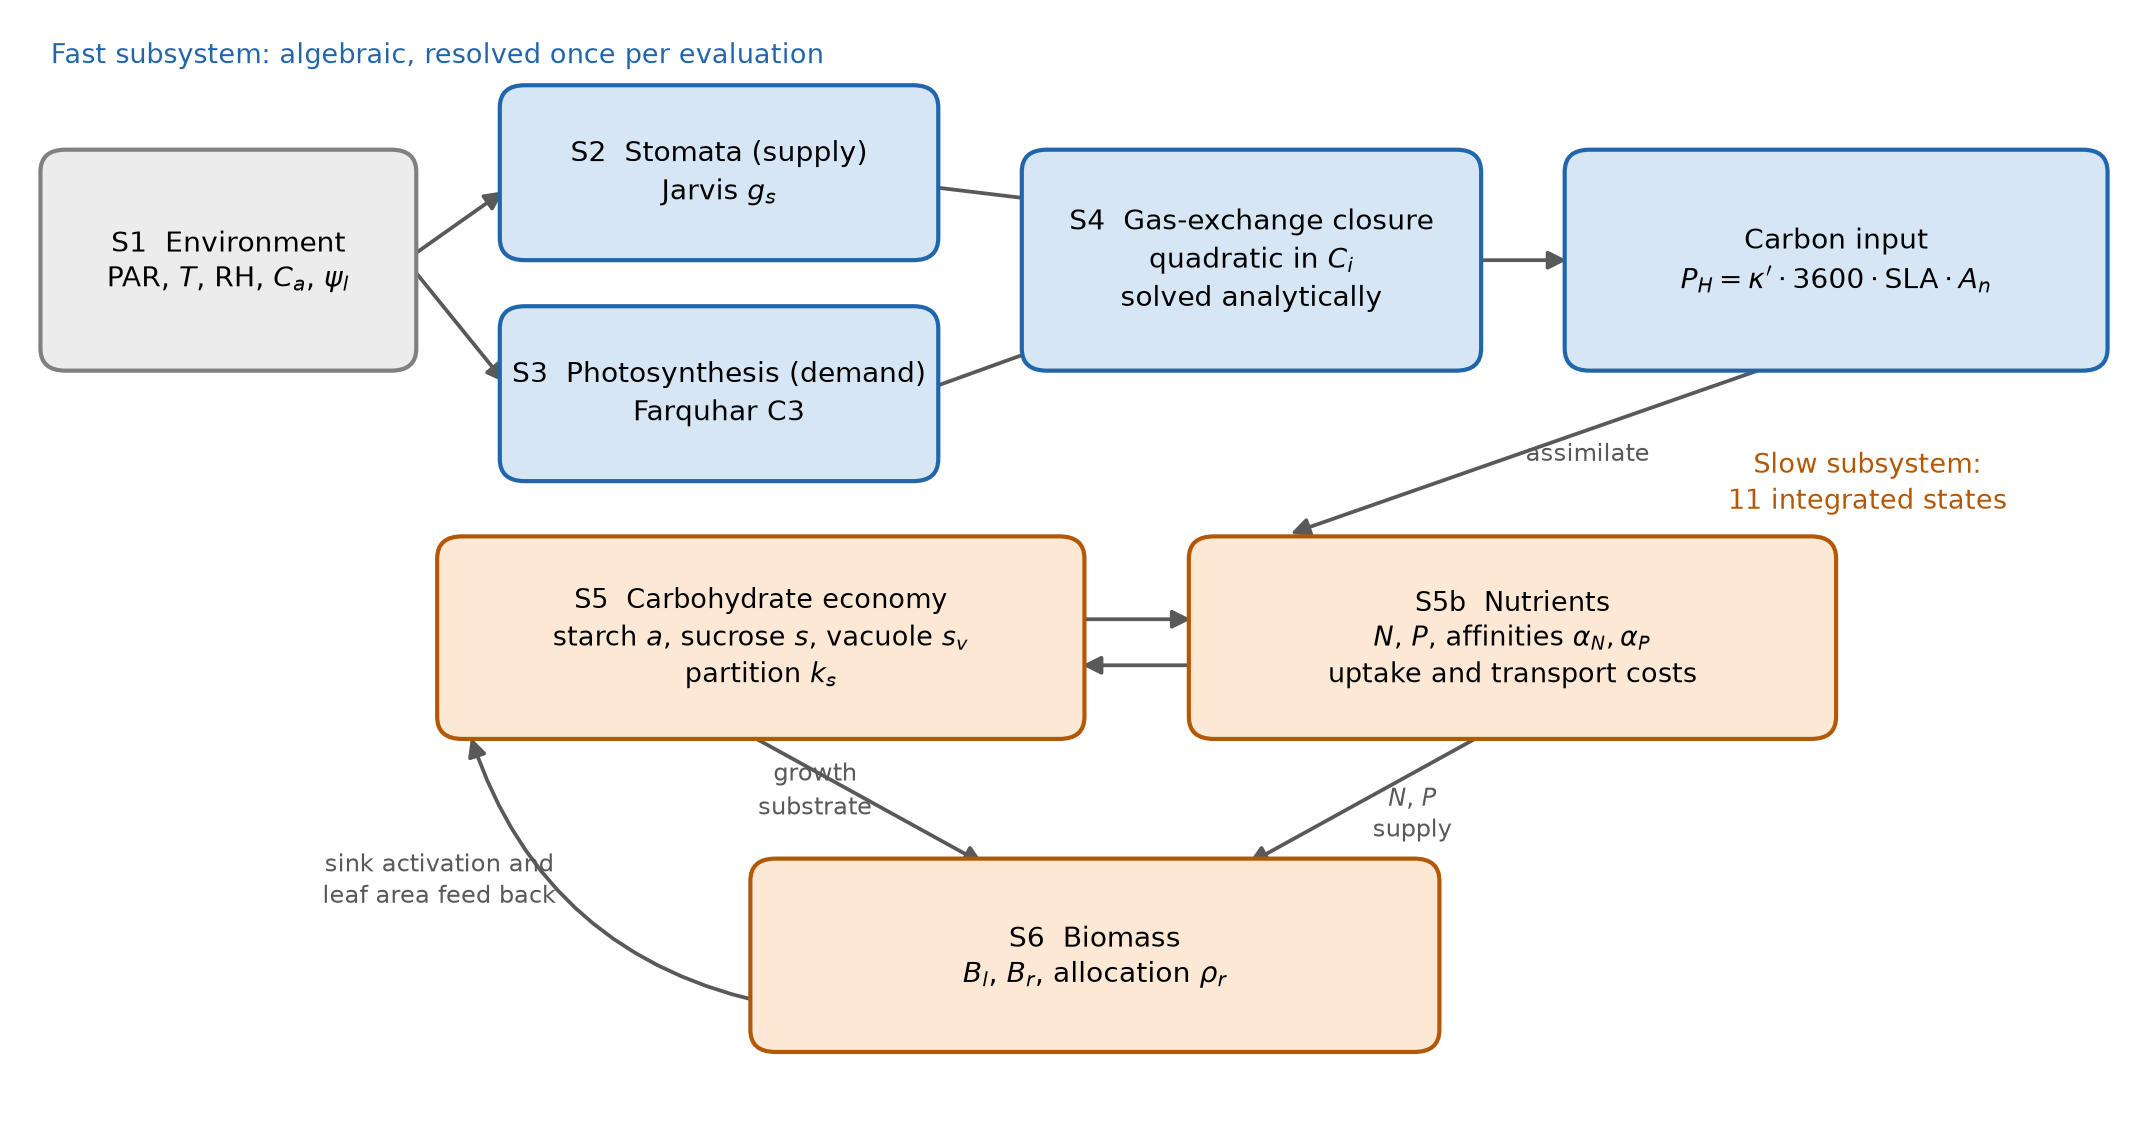
\includegraphics[width=\textwidth]{model_overview.png}
\caption{Model architecture and information flow through one derivative
evaluation. The fast subsystem (blue) is algebraic and is resolved once per
evaluation: environmental forcing S1 drives the stomatal supply function S2 and
the photosynthetic demand function S3, which are closed against each other in S4
as a quadratic in the intercellular CO$_2$ concentration and solved in closed
form. The resulting net assimilation is converted to the model carbon input
$P_H$. The slow subsystem (orange) comprises the eleven integrated states: the
carbohydrate economy S5, nutrient acquisition with its explicit costs S5b, and
leaf and root biomass S6. Growth returns to the carbohydrate economy through
sink activation and through leaf area, which closes the only feedback loop in the
architecture. Arrows show the direction of information flow, not stoichiometric
mass transfer; the carbon budget is stated in
Section~\ref{sec:carbon_closure}.}
\label{fig:overview}
\end{figure*}

\subsection{Conceptual model and system decomposition}
\label{sec:conceptual}

The system is a single vegetative \textit{Arabidopsis} plant with its immediate
physical environment. Radiation, air temperature, humidity, ambient CO$_2$, leaf
water potential and soil nutrient concentrations cross the boundary as external
inputs. Carbon and nutrient acquisition, storage and allocation to leaf and root
biomass are internal states. The plant is two mass compartments, leaf and root,
without explicit geometry, so internal transport is described by aggregate
pools. This lumped decomposition and the carbon--nutrient allocation states
follow the whole-plant growth framework of \citet{Tedone2020}, whose prescribed
carbon input is here replaced by a computed gas-exchange layer.

Figure~\ref{fig:overview} shows the decomposition into six submodels and the
signals they exchange.
\begin{enumerate}\itemsep2pt
\item[\textbf{S1}] \emph{Environmental forcing} maps clock time to the light switch
      and the micro-climate. \emph{In:} $t$, scenario parameters. \emph{Out:}
      $\mathit{PAR}$, $T$, $\mathit{RH}$, $\mathit{VPD}$, $C_a$, $\psi_w$, $L$.
\item[\textbf{S2}] \emph{Stomatal conductance (supply)}, a multiplicative Jarvis
      model. \emph{In:} $\mathit{PAR}$, $\mathit{VPD}$, $T$, $C_a$, $\psi_w$.
      \emph{Out:} $g_s$.
\item[\textbf{S3}] \emph{Leaf photosynthesis (demand)}, the Farquhar C$_3$ model.
      \emph{In:} $\mathit{PAR}$, $C_i$, $V_{c\max}$, $J_{\max}$. \emph{Out:}
      $A_n(C_i)$.
\item[\textbf{S4}] \emph{Gas-exchange coupling} closes supply against demand.
      \emph{In:} $g_s$, $A_n(C_i)$, $C_a$. \emph{Out:} $A_n$, $C_i$.
\item[\textbf{S5}] \emph{Carbohydrate and nutrient economy} holds the diel starch
      and sucrose pools, the vacuolar compartment, and sucrose-limited N and P
      uptake with its costs. \emph{In:} $\Phi_c$, soil $N_s$, $P_s$. \emph{Out:}
      $s$, $U_N$, $U_P$.
\item[\textbf{S6}] \emph{Growth and allocation} converts exported sucrose into
      leaf and root biomass under functional-balance control. \emph{In:} $s$,
      $\alpha_N$, $\alpha_P$, $\varsigma$. \emph{Out:} $B_l$, $B_r$, $\rho_r$.
\end{enumerate}

Submodels S2--S4 form a fast algebraic subsystem. Leaf gas exchange equilibrates
within seconds, so it is treated as instantaneously relaxed relative to the slow
states in S5 and S6, which evolve over the diel cycle. It is therefore not
integrated but evaluated in closed form at every derivative call, as an
algebraic constitutive layer inside the derivative of the slow states
\citep{Cellier1991,Zeigler2000}. This separation organises both the formulation
and the implementation.

Only one signal returns from the slow subsystem to the fast one: leaf biomass
$B_l$ acts as a viability gate, and the carbon input is zero when
$B_l < B_{l,\min}$. The photosynthetic capacities $V_{c\max}$ and $J_{\max}$ are
fixed parameters and do not respond to nitrogen or carbohydrate status.
Figure~\ref{fig:overview} must therefore not be read as showing a capacity
feedback that the equations do not contain.

The formulation rests on six assumptions.
\begin{enumerate}\itemsep1pt
\item[(A1)] The plant is lumped into leaf and root compartments; no within-organ
      gradients or canopy architecture are resolved.
\item[(A2)] Leaf gas exchange is at steady state at every instant, so
      intercellular CO$_2$ is an algebraic balance and not a state.
\item[(A3)] Stomatal conductance responds multiplicatively to the environment and
      not to the assimilation rate \citep{Jarvis1976,Damour2010}.
\item[(A4)] Transitory starch is mobilised at a nocturnal rate paced by night
      length, as the observed near-linear depletion indicates
      \citep{Graf2010,Scialdone2013}.
\item[(A5)] Active nutrient uptake is limited by cytosolic sucrose, so carbon and
      nutrient acquisition are co-limiting \citep{Smith2007}.
\item[(A6)] Partitioning follows functional-balance theory: investment shifts
      towards the most limiting resource
      \citep{Thornley1972,ThornleyJohnson1990}.
\end{enumerate}

\subsection{State-space representation}
\label{sec:state}

The slow states form the vector $X(t)\in\mathbb{R}^{11}$ governed by

\begin{equation}
\frac{dX(t)}{dt} = f\!\left(X(t),\,U(t),\,\boldsymbol{\theta},\,t\right),
\label{eq:ode_general}
\end{equation}

where $U(t)$ is the exogenous forcing and $\boldsymbol{\theta}$ the time-invariant
parameter set. The explicit time dependence enters only through the diel forcing. In
the order used by the state packing routine of the implementation,

\begin{equation}
X(t) =
\left[
k_s,\; a,\; s,\; \alpha_N,\; \alpha_P,\; N,\; P,\; \rho_r,\; B_l,\; B_r,\; s_v
\right]^{\mathsf{T}}.
\label{eq:state_vector}
\end{equation}

Each symbol is defined in Table~\ref{tab:states}. Total biomass $B = B_l + B_r$ is
recomputed from the two biomass states whenever it is needed and is not integrated
as a twelfth state.

The pool states $a$, $s$, $s_v$, $N$ and $P$ are normalised model pools on a
nominal per-fresh-weight basis, not concentrations of a growing body. We adopt
this reading because it is the one under which the implemented balance equations
are exact: no growth-dilution term appears in Eqs.~\eqref{eq:starch},
\eqref{eq:sucrose}, \eqref{eq:sucrose_vac}, \eqref{eq:dN} or~\eqref{eq:dP}. The
cost is that $a$ and $s$ are not directly measured tissue concentrations, so the
carbohydrate comparison in Section~\ref{sec:results} is a comparison of shape and
timing after multiplicative alignment, not of absolute level.

The forcing vector is

\begin{equation}
U(t) =
\left[
\mathit{PAR}(t),\; T(t),\; \mathit{RH}(t),\; \mathit{VPD}(t),\; C_a,\;
\psi_w,\; L(t)
\right]^{\mathsf{T}},
\label{eq:input_vector}
\end{equation}

The deficit $\mathit{VPD}$ is a diagnostic function of $T$ and $\mathit{RH}$
through Eq.~\eqref{eq:vpd} and is not an independent input; it is listed because it
enters the stomatal response directly. In the scenarios reported here $T$,
$\mathit{RH}$, $C_a$ and $\psi_w$ are constant, so the only time-varying inputs are
$\mathit{PAR}$ and $L$.

\begin{table}[!htbp]
\centering
\small
\caption{State variables, environmental inputs and the principal derived
quantities. Pool states are normalised model pools on a nominal per-fresh-weight
basis (Section~\ref{sec:state}). ``Derived'' quantities are recomputed
algebraically at every derivative evaluation and are not integrated.}
\label{tab:states}
\begin{tabular}{@{}lllp{34mm}@{}}
\toprule
Symbol & Meaning & Unit & Role \\
\midrule
$k_s$        & Starch partition coefficient       & --                            & state, Eq.~\eqref{eq:dks} \\
$a$          & Transitory starch pool             & $\mu\mathrm{mol\,C_6\,gFW^{-1}}$ & state, Eq.~\eqref{eq:starch} \\
$s$          & Cytosolic sucrose pool             & $\mu\mathrm{mol\,C_6\,gFW^{-1}}$ & state, Eq.~\eqref{eq:sucrose} \\
$s_v$        & Vacuolar sucrose pool              & $\mu\mathrm{mol\,C_6\,gFW^{-1}}$ & state, Eq.~\eqref{eq:sucrose_vac} \\
$\alpha_N$   & Nitrogen investment state          & --                            & state, Eq.~\eqref{eq:dalphaN} \\
$\alpha_P$   & Phosphorus investment state        & --                            & state, Eq.~\eqref{eq:dalphaP} \\
$N$          & Internal nitrogen pool             & $\mu\mathrm{mol\,N\,gFW^{-1}}$ & state, Eq.~\eqref{eq:dN} \\
$P$          & Internal phosphorus pool           & $\mu\mathrm{mol\,P\,gFW^{-1}}$ & state, Eq.~\eqref{eq:dP} \\
$\rho_r$     & Sucrose-to-root allocation state   & --                            & state, Eq.~\eqref{eq:drhor} \\
$B_l$        & Leaf biomass                       & gFW                           & state, Eq.~\eqref{eq:dBl} \\
$B_r$        & Root biomass                       & gFW                           & state, Eq.~\eqref{eq:dBr} \\
\midrule
$\mathit{PAR}$ & Photosynthetically active radiation & $\mu\mathrm{mol\,m^{-2}\,s^{-1}}$ & input, Eq.~\eqref{eq:par_profile} \\
$L$          & Light/dark switch                  & --                            & input, Eq.~\eqref{eq:photoperiod} \\
$T$          & Leaf temperature                   & $^\circ$C                     & input, constant \\
$\mathit{RH}$& Relative humidity                  & \%                            & input, constant \\
$C_a$        & Ambient CO$_2$ concentration       & $\mu\mathrm{mol\,mol^{-1}}$   & input, constant \\
$\psi_w$     & Leaf water potential               & MPa                           & input, constant \\
$N_s,P_s$    & Soil N, P concentration            & $\mu\mathrm{mol\,cm^{-3}}$    & input, constant \\
\midrule
$\mathit{VPD}$ & Vapour pressure deficit          & kPa                           & derived, Eq.~\eqref{eq:vpd} \\
$g_s,g_c$    & Conductance to H$_2$O, to CO$_2$   & $\mathrm{mol\,m^{-2}\,s^{-1}}$& derived, Eqs.~\eqref{eq:jarvis}, \eqref{eq:supply} \\
$C_i$        & Intercellular CO$_2$ concentration & $\mu\mathrm{mol\,mol^{-1}}$   & derived, Eq.~\eqref{eq:ci_root} \\
$A_c,A_j$    & Rubisco-, RuBP-limited rate        & $\mu\mathrm{mol\,m^{-2}\,s^{-1}}$ & derived, Eqs.~\eqref{eq:Ac}, \eqref{eq:Aj} \\
$A_n$        & Net leaf assimilation              & $\mu\mathrm{mol\,m^{-2}\,s^{-1}}$ & derived, Eq.~\eqref{eq:An} \\
$J$          & Electron transport rate            & $\mu\mathrm{mol\,m^{-2}\,s^{-1}}$ & derived, Eq.~\eqref{eq:J_root} \\
$\Phi_c$     & Carbon input to the pools          & $\mu\mathrm{mol\,C_6\,gFW^{-1}\,h^{-1}}$ & derived, Eq.~\eqref{eq:conversion} \\
$D_a$        & Starch degradation flux            & $\mu\mathrm{mol\,C_6\,gFW^{-1}\,h^{-1}}$ & derived, Eq.~\eqref{eq:starch_degradation} \\
$E$          & Exportable sucrose term            & $\mu\mathrm{mol\,C_6\,gFW^{-1}}$ & derived, Eq.~\eqref{eq:export} \\
$U_N,U_P$    & Realised N, P uptake               & $\mu\mathrm{mol\,gFW^{-1}\,h^{-1}}$ & derived, Eq.~\eqref{eq:uptake} \\
$\varsigma$  & Stoichiometric signal              & --                            & derived, Eq.~\eqref{eq:stoich} \\
$B$          & Total biomass, $B_l+B_r$           & gFW                           & derived \\
\bottomrule
\end{tabular}
\end{table}

\subsection{Submodel S1: environmental forcing}
\label{sec:forcing}

Let $h(t) = t \bmod 24$ be the hour of day and $f$ the photoperiod length in
hours. The light switch is

\begin{equation}
L(t) =
\begin{cases}
1, & 0 \leq h(t) < f, \\
0, & f \leq h(t) < 24 ,
\end{cases}
\label{eq:photoperiod}
\end{equation}

and the incident radiation follows one of two daytime profiles, selected by
scenario:

\begin{equation}
\mathit{PAR}(t) =
\begin{cases}
\mathit{PAR}_{\max}, & \text{square wave},\; L=1, \\[4pt]
\mathit{PAR}_{\max}\,\sin\!\left(\pi\,h(t)/f\right), & \text{half sine},\; L=1, \\[4pt]
0, & L=0 .
\end{cases}
\label{eq:par_profile}
\end{equation}

The square wave represents a growth chamber, which delivers constant irradiance
over the light period; the half sine is a smooth idealisation of a natural light
course. The choice sets the daily light integral: the square wave gives
$\mathit{PAR}_{\max} f$ and the half sine $(2/\pi)\,\mathit{PAR}_{\max} f$. A run
matching a chamber experiment must therefore use the square profile at the
chamber irradiance. One consequence of the design affects every photoperiod
result. With $\mathit{PAR}_{\max}$ held fixed, changing the photoperiod changes
the daily light integral in proportion. Day length and daily photon dose are
confounded by construction, so a photoperiod response in this model is a joint
response to duration and dose.

The vapour pressure deficit is obtained from leaf temperature and relative
humidity through the Tetens relation \citep{Monteith1965,Nobel2009},

\begin{equation}
\mathit{VPD} = e_s\left(1 - \frac{\mathit{RH}}{100}\right),
\qquad
e_s = 0.61078\,\exp\!\left(\frac{17.27\,T}{T + 237.3}\right),
\label{eq:vpd}
\end{equation}

with $e_s$ and $\mathit{VPD}$ in kPa and $T$ in $^\circ$C. Where a
thermoperiod is specified, $T$ takes its day value while $L=1$ and its night
value while $L=0$; otherwise $T$ is constant.

\subsection{Submodel S2: stomatal conductance (supply)}
\label{sec:jarvis}

This submodel returns the stomatal conductance and forms the supply side of gas
exchange. It carries no dependence on the assimilation rate (A3). Conductance
is a maximal value reduced by a product of dimensionless environmental
modifiers, each bounded in $[0,1]$ \citep{Jarvis1976,Damour2010}:

\begin{equation}
g_s = g_{s,\max}\;
f_{\mathit{PAR}}(\mathit{PAR})\;
f_{\mathit{VPD}}(\mathit{VPD})\;
f_T(T)\;
f_{\mathit{CO_2}}(C_a)\;
f_w(\psi_w).
\label{eq:jarvis}
\end{equation}

The multiplicative closure assumes that the environmental controls act
independently. It is a widely used empirical conductance model and needs no
optimisation step at runtime \citep{Damour2010,Buckley2017}. The maximal
conductance $g_{s,\max}$ is a separate parameter from the shape parameters of the
modifiers. Each modifier can then be required to equal unity at its own
non-limiting reference condition, so changing the shape of one modifier does not
rescale the whole conductance.

The light response is a saturating hyperbola with a residual conductance
$b_{10}$ below a breakpoint $q = b_{10}/b_1$,

\begin{equation}
f_{\mathit{PAR}} =
\begin{cases}
b_{10}, & \mathit{PAR} \leq q, \\[6pt]
\dfrac{b_1 b_2\,(\mathit{PAR}-q)}{b_1 + b_2\,(\mathit{PAR}-q)}, & \mathit{PAR} > q .
\end{cases}
\label{eq:jarvis_par}
\end{equation}

The response to atmospheric demand is linear and floored at zero, and the
response to leaf water potential is a saturating recovery above a closure
potential $\psi_{\min}$, clipped to $[0,1]$:

\begin{align}
f_{\mathit{VPD}} &= \max\!\left(0,\; 1 - b_5\,\mathit{VPD}\right),
\label{eq:jarvis_vpd}\\[4pt]
f_w &= 1 - \exp\!\left(-b_6\,(\psi_w - \psi_{\min})\right).
\label{eq:jarvis_water}
\end{align}

The temperature response is a skewed optimum with zeros at $T_1$ and $T_h$,

\begin{equation}
f_T =
\begin{cases}
b_3\,(T - T_1)\,(T_h - T)^{b_4}, & T_1 < T < T_h, \\[4pt]
0, & \text{otherwise},
\end{cases}
\qquad
b_4 = \frac{T_h - T_0}{T_0 - T_1},
\quad
b_3 = \frac{1}{(T_0 - T_1)(T_h - T_0)^{b_4}} .
\label{eq:jarvis_T}
\end{equation}

The two constants $b_3$ and $b_4$ are not free. They are fixed by requiring
stationarity at $T_0$ and $f_T(T_0)=1$, which places the maximum at $T_0$ and
normalises the modifier to unity there. With $T_1 = 5$, $T_0 = 25$ and
$T_h = 45\,^\circ$C this gives $b_4 = 1$, so the curve is a single-peaked
parabola and no clipping from above is needed.

The CO$_2$ response is piecewise linear in $C_a$, expressed in
$\mu\mathrm{mol\,mol^{-1}}$. It is constant below $100$, falls linearly to a floor
$b_8$ at $1000$, and equals that floor above it:

\begin{equation}
f_{\mathit{CO_2}} =
\begin{cases}
1, & C_a < 100, \\[4pt]
1 - b_7\,(C_a - 100), & 100 \leq C_a < 1000, \\[4pt]
b_8, & C_a \geq 1000,
\end{cases}
\qquad
b_7 = \frac{1 - b_8}{900} .
\label{eq:jarvis_co2}
\end{equation}

\subsection{Submodel S3: leaf photosynthesis (demand)}
\label{sec:farquhar}

This submodel returns net assimilation as a function of the intercellular
CO$_2$ concentration and forms the demand side of gas exchange. It is the
Farquhar--von~Caemmerer--Berry C$_3$ model, in which gross assimilation is the
smaller of a Rubisco-limited and an electron-transport-limited rate
\citep{Farquhar1980,vonCaemmerer2000}. The Rubisco-limited rate is

\begin{equation}
A_c = V_{c\max}\,
\frac{C_i - \Gamma^{*}}{C_i + K_c\!\left(1 + O/K_o\right)},
\label{eq:Ac}
\end{equation}

with $\Gamma^{*}$ the CO$_2$ compensation point in the absence of dark
respiration, $K_c$ and $K_o$ the Michaelis constants of Rubisco for CO$_2$ and
O$_2$, and $O$ the oxygen concentration. The electron-transport-limited rate is

\begin{equation}
A_j = J\,\frac{C_i - \Gamma^{*}}{4.5\,C_i + 10.5\,\Gamma^{*}},
\label{eq:Aj}
\end{equation}

where the denominator coefficients $4.5$ and $10.5$ encode the electron
requirement per carboxylation and per oxygenation under the standard
stoichiometry of RuBP regeneration
\citep{vonCaemmerer1981,vonCaemmerer2000}. Net assimilation is the limiting
rate less dark respiration,

\begin{equation}
A_n = \min(A_c,\,A_j) - R_d .
\label{eq:An}
\end{equation}

The electron transport rate follows from $\mathit{PAR}$ through the
non-rectangular hyperbola
$\theta J^2 - (J_{\max} + \phi\,\mathit{PAR})J + J_{\max}\phi\,\mathit{PAR} = 0$
\citep{Farquhar1980,Farquhar1984}, of which the lower root is taken,

\begin{equation}
J = \frac{\left(J_{\max}+\phi\,\mathit{PAR}\right)
- \sqrt{\left(J_{\max}+\phi\,\mathit{PAR}\right)^{2}
- 4\,\theta\,J_{\max}\,\phi\,\mathit{PAR}}}{2\,\theta},
\label{eq:J_root}
\end{equation}

with $\phi$ the apparent quantum yield for electron transport and $\theta$ the
curvature of the light response.

No irradiance threshold is applied to this submodel: the carbon input is evaluated
whenever $\mathit{PAR} > 0$ and $B_l \geq B_{l,\min}$. A threshold is unnecessary
because, with the closed-form operating point of Section~\ref{sec:closure}, the net
rate passes continuously through zero at the light compensation point and the clamp
in Eq.~\eqref{eq:conversion} returns exactly zero below it. Below that point $A_n$
itself remains negative. It is the carbon input that is clamped and not $A_n$, so
respiratory efflux is never counted as an assimilatory gain.

\subsection{Submodel S4: gas-exchange coupling}
\label{sec:closure}

Equations~\eqref{eq:Ac}--\eqref{eq:An} give demand as a function of a
concentration that is itself set by supply. Fickian diffusion of CO$_2$ through
the stomata gives

\begin{equation}
A_n = g_c\,(C_a - C_i),
\qquad
g_c = \frac{g_s}{1.6},
\label{eq:supply}
\end{equation}

where the factor $1.6$ converts the conductance to water vapour into a conductance
to CO$_2$, which diffuses more slowly in air \citep{vonCaemmerer2000,Nobel2009}.
Because $A_n$ depends on $C_i$ and $C_i$ depends on $A_n$, the operating point is
the mutual solution of Eqs.~\eqref{eq:An} and~\eqref{eq:supply}. How that coupling
is solved is the main methodological choice in the formulation.

The system needs no iteration. Both Farquhar branches have the same rational form
in $C_i$,

\begin{equation}
A = \frac{\mathrm{num}\,(C_i - \Gamma^{*})}{d_1 C_i + d_0} - R_d,
\qquad
(\mathrm{num},\,d_1,\,d_0) =
\begin{cases}
\bigl(V_{c\max},\; 1,\; K_c(1 + O/K_o)\bigr), & \text{Rubisco branch}, \\[4pt]
\bigl(J,\; 4.5,\; 10.5\,\Gamma^{*}\bigr), & \text{transport branch},
\end{cases}
\label{eq:branch_form}
\end{equation}

so the branch coefficients are read directly off Eqs.~\eqref{eq:Ac}
and~\eqref{eq:Aj} without dividing through. Equating supply and demand,

\begin{equation}
g_c\,(C_a - C_i)\,(d_1 C_i + d_0)
= \mathrm{num}\,(C_i - \Gamma^{*}) - R_d\,(d_1 C_i + d_0),
\label{eq:closure_raw}
\end{equation}

and clearing the denominator gives a quadratic in $C_i$,

\begin{equation}
a\,C_i^{2} + b\,C_i + c = 0,
\qquad
\begin{aligned}
a &= -g_c\,d_1, \\
b &= g_c\,(d_1 C_a - d_0) - \mathrm{num} + R_d\,d_1, \\
c &= g_c\,d_0\,C_a + \mathrm{num}\,\Gamma^{*} + R_d\,d_0 .
\end{aligned}
\label{eq:ci_quadratic}
\end{equation}

Exactly one root of Eq.~\eqref{eq:ci_quadratic} is admissible on each branch, and
no search is needed to identify it. The admissibility condition is $C_i \geq 0$
alone. For $g_c > 0$ the leading coefficient is $a = -g_c d_1 < 0$, while $c > 0$
because every factor in it is positive. The product of the roots $c/a$ is
therefore negative, so each branch has one positive and one negative root, and the
positive one is the operating point:

\begin{equation}
C_i =
\frac{-b - \sqrt{b^{2} - 4ac}}{2a}
\;>\; 0 .
\label{eq:ci_root}
\end{equation}

Substituting this root back into Eq.~\eqref{eq:branch_form} gives the branch
assimilation, and the smaller of the two branch values is returned. That is the
same co-limitation rule as $\min(A_c,A_j)$ in Eq.~\eqref{eq:An}, applied after
each branch has been closed against supply rather than before. Because exactly one
root per branch is admissible, the minimum over the two branches is the solution
of the coupled system and not merely a candidate for it.

The admissibility rule deserves emphasis, because the natural guess is wrong. No
upper bound on $C_i$ is imposed, and a root above the ambient concentration is
retained rather than rejected. By Eq.~\eqref{eq:supply}, $C_i > C_a$ is exactly
what the supply relation returns whenever $A_n < 0$, that is, whenever the leaf is
a net source and CO$_2$ diffuses outward. The condition $0 \le C_i \le C_a$ is
therefore not a physical constraint here, and imposing it would discard the
correct root twice a day.

The vanishing-conductance case has a physical answer rather than a clamp. As
$g_c \to 0$ the quadratic degenerates, with $a \to 0$ and $b \to -\mathrm{num}$,
and the finite root of the remaining linear equation gives
$C_i \to \Gamma^{*} + R_d d_0/\mathrm{num}$, at which Eq.~\eqref{eq:branch_form}
returns $A = -R_d$. Closed stomata admit no CO$_2$, so the leaf only respires. The
implementation returns this limit directly at the boundary $g_c \leq 0$,

\begin{equation}
C_i = \Gamma^{*}, \qquad A_n = -R_d ,
\label{eq:ci_dark}
\end{equation}

which is the correct dark limit and replaces a clamp on the conductance.
Respiration in low light and darkness is then carried by the same expression that
carries assimilation in the light, with no special case and no discontinuity in
$A_n$ at the light compensation point.

Two properties of this closure matter for the rest of the paper. The branch-wise
quadratic is solved once per derivative evaluation, with no inner iteration in the
production configuration, so the derivative is a deterministic function of $(X,t)$
as an embedded-pair error estimate assumes. And the solution is exact up to
floating-point arithmetic, so no inner convergence tolerance interacts with the
outer error control. Section~\ref{sec:implementation} reports the substitution
residual that verifies this.

\subsection{From assimilation to model carbon input}
\label{sec:conversion}

The leaf-level net assimilation $A_n$
($\mu\mathrm{mol\,CO_2\,m^{-2}\,s^{-1}}$) must be converted to the carbon
input $\Phi_c$ that drives the carbohydrate pools
($\mu\mathrm{mol\,C_6\,gFW^{-1}\,h^{-1}}$). The conversion is

\begin{equation}
\Phi_c = \Lambda\;\max\!\left(0,\;
\underbrace{\mathrm{SLA}}_{\mathrm{m^2\,gFW^{-1}}}\;
\underbrace{\frac{3600}{6}}_{\mathrm{s\,h^{-1}\ /\ mol\,CO_2\,per\,mol\,C_6}}\;
A_n \right),
\qquad L = 1 ,
\label{eq:conversion}
\end{equation}

and $\Phi_c = 0$ when $L = 0$ or $B_l < B_{l,\min}$. Three factors carry the whole
unit conversion and none of them is free: $\mathrm{SLA}$ moves the flux to a
per-fresh-weight basis, the factor $3600$ converts seconds to hours, and the
divisor $6$ converts moles of CO$_2$ to moles of hexose. Their product is
$600\,\mathrm{SLA}$, so at the measured $\mathrm{SLA}$ of Table~\ref{tab:params}
the coefficient is fixed by the units and no empirical scaling constant enters the
carbon-input pathway. The clamp keeps a negative $A_n$ out of the pools, as
discussed in Section~\ref{sec:farquhar}.

The factor $\Lambda$ is a sink-limitation term that down-regulates assimilation
as the starch pool fills,

\begin{equation}
\Lambda = \min\!\left(1,\; \max\!\left(\lambda_c,\;
\lambda_c + (1-\lambda_c)\,\frac{a_{\max} - a}{a_{\max}}\right)\right),
\qquad
a_{\max} = D_{a,\max}\,(24 - f),
\label{eq:feedback}
\end{equation}

where $\lambda_c$ is the residual assimilation fraction at a full pool and the
ceiling $a_{\max}$ scales with night length, since a longer night requires a
larger reserve. The inner $\max$ bounds the term at its value at the ceiling, so a
pool above $a_{\max}$ cannot drive $\Lambda$ negative and reverse the sign of
assimilation. In all reported runs $\lambda_c = 1$, which makes $\Lambda = 1$
identically and the sink limitation inactive. The equation is given because the
term is present in the right-hand side and is used in the ablation of
Section~\ref{sec:protocol}; its shipped value is stated so that a reader knows
the reported results do not depend on it.

\subsection{Submodel S5: carbohydrate economy}
\label{sec:carbohydrates}

The carbon input $\Phi_c$ is split between transitory starch and cytosolic sucrose
by the partition coefficient $k_s$. This coefficient is a state with its own
dynamics rather than a fixed split, so the plant can shift it during the day and
again at night in response to the sucrose level. The diel carbohydrate balance is
then an emergent property of the model and not a prescribed schedule
\citep{Stitt2012,Mengin2017}.

\paragraph{Starch partition.}
Let $\sigma^{-} = s_{\min}/(s_{\min}+s)$ and
$\sigma^{+} = s/(s+s_{\max})$ be the sucrose-deficit and sucrose-excess
fractions, both in $[0,1]$ and both saturating. The partition state follows

\begin{equation}
\frac{dk_s}{dt}
= \underbrace{L\left[
-\,k_s\,\lambda_{sdr}\,\sigma^{-}
+\left(1-k_s\right)\lambda_{sdi}\,\sigma^{+}
\right]}_{\text{light phase}}
+\underbrace{\left(1-L\right)\left(1-k_s\right)\lambda_{sni}\,\sigma^{-}}_{\text{dark phase}} .
\label{eq:dks}
\end{equation}

Each term has a direct interpretation. In the light, a low sucrose level makes
$\sigma^{-}$ large and the first term reduces $k_s$, so more incoming carbon goes
to sucrose and the immediate demand is met. A high sucrose level makes
$\sigma^{+}$ large and the second term raises $k_s$, so surplus carbon is stored
as starch. In the dark there is no input to partition, and the third term raises
$k_s$ when sucrose is low, returning the state to a storage-biased value before
the next light period. The factors $k_s$ and $(1-k_s)$ keep the state in $[0,1]$
without a clamp, since each term vanishes at the bound it approaches. The three
rate coefficients set the speed of the day-reduction, day-increase and
night-increase responses.

\paragraph{Starch pool.}
Starch gains the partitioned share of the input and loses the nocturnal
degradation flux $D_a$,

\begin{equation}
\frac{da}{dt} = k_s\,\Phi_c - D_a .
\label{eq:starch}
\end{equation}

The degradation flux implements the observed pacing of starch mobilisation
against the remaining night length \citep{Graf2010,Scialdone2013}. Let
$a_{\mathrm{dusk}}$ be the starch content recorded at the last transition to
darkness and $a_{\min}$ the residual pool that is not mobilised. Then

\begin{equation}
D_a =
\left(1-L\right)
\min\!\left(
D_{a,\max},\;
\left[
\frac{h}{24} + \left(1-\frac{h}{24}\right)\left(1-\frac{s}{s+s_{\max}}\right)
\right]
\frac{a_{\mathrm{dusk}} - a_{\min}}{24 - f}
\right),
\label{eq:starch_degradation}
\end{equation}

and $D_a = 0$ if $a_{\mathrm{dusk}} < a_{\min}$. The quotient
$(a_{\mathrm{dusk}}-a_{\min})/(24-f)$ is the constant rate that would exactly
exhaust the mobilisable reserve over the night, which is the rate the
measurements show. The bracketed factor modulates it: when sucrose is abundant
the second summand is small and degradation is slowed, so the reserve is spared.
The outer $\min$ bounds the flux by the degradation capacity $D_{a,\max}$ and the
factor $(1-L)$ confines it to darkness. Two properties matter for the limitation
reported in Section~\ref{sec:limitations}. The reference level
$a_{\mathrm{dusk}}$ is sampled at dusk and held over the night, so it is not a
continuous function of the state, and the divisor $24-f$ is the nominal rather
than the remaining night length.

\paragraph{Sucrose pools.}
Cytosolic sucrose receives the unpartitioned share of the input and the starch
degradation flux, and pays four costs: nutrient uptake, phloem transport,
maintenance respiration, and export to the sinks. It also exchanges with the
vacuolar pool. The balance is

\begin{equation}
\frac{ds}{dt}
= \left(1-k_s\right)\Phi_c
+ D_a
- C_u
- C_t
- R_m
- \eta\,E
- k_{\mathrm{in}}\,s
+ k_{\mathrm{out}}\,s_v
- C_g ,
\label{eq:sucrose}
\end{equation}

\begin{equation}
\frac{ds_v}{dt} = k_{\mathrm{in}}\,s - k_{\mathrm{out}}\,s_v .
\label{eq:sucrose_vac}
\end{equation}

The vacuolar compartment is a passive first-order buffer with influx rate
$k_{\mathrm{in}}$ and efflux rate $k_{\mathrm{out}}$, and the two rate constants
appear with opposite signs in Eqs.~\eqref{eq:sucrose} and~\eqref{eq:sucrose_vac},
so the exchange conserves sucrose. It represents the measured separation of leaf
sucrose into an active cytosolic fraction and a larger stored vacuolar fraction
\citep{Lohaus2000,Nadwodnik2008}. Only $s$ enters the cost and export terms, so
the buffer damps the diel excursion of the active pool without adding or removing
carbon, with relaxation time $1/(k_{\mathrm{in}}+k_{\mathrm{out}})$.

The export term is the phloem-loading flux, and it carries the sugar-induced
sink activation:

\begin{equation}
E =
\underbrace{\min\!\left(s,\;s_{\max}\right)}_{\text{loadable pool}}
\underbrace{\left[1 + \left(\frac{s}{K_s}\right)^{n_H}\right]}_{\text{sink activation}}
\underbrace{\left[\lambda_g + \left(1-\lambda_g\right)\left(1 - L + L\left(1-k_s\right)\right)\right]}_{\text{loading efficiency}} .
\label{eq:export}
\end{equation}

The activation factor multiplies the loadable pool before the loading efficiency
is applied, so it scales the export flux and not the pool size. Its form requires
comment because it is not the bounded Hill function. A saturating factor
$s^{n_H}/(K_s^{n_H}+s^{n_H})$ is bounded above by one and can therefore only
weaken the drain, which is the wrong direction. Sucrose induces its own
consumption, by raising invertase activity and sink-tissue transporter
expression, so consumption capacity rises with the pool
\citep{Smith2007,Stitt2012}. The unbounded factor $1+(s/K_s)^{n_H}$ represents
this: it is close to one at $s \ll K_s$, and at $s \gg K_s$ the drain scales as
$s^{1+n_H}$. The steady-state pool then grows as the $1/(1+n_H)$ power of the
supply, so the sucrose level is held near $K_s$ while assimilation varies. A
first-order drain with constant coefficients cannot hold a level in this way. The
half-activation constant $K_s$ is one of the four calibrated parameters
(Table~\ref{tab:fitted}).

The loading efficiency term interpolates between a floor $\lambda_g$ and unity.
It equals one at night and $\lambda_g + (1-\lambda_g)(1-k_s)$ in the light, so
export is least efficient when the light-phase partition is strongly biased to
starch. The remaining costs are

\begin{align}
C_u &= c_N\,U_N + c_P\,U_P ,
\label{eq:uptake_cost}\\[3pt]
C_t &= \tau_c\left(r_m\,s + \eta\,E\right),
\label{eq:transport_cost}\\[3pt]
R_m &= r_m\,s ,
\label{eq:respiration}\\[3pt]
C_g &=
\begin{cases}
Y\left(\dfrac{dB_l}{dt} + \dfrac{dB_r}{dt}\right), &
\dfrac{dB_l}{dt} + \dfrac{dB_r}{dt} > 0, \\[10pt]
0, & \text{otherwise} .
\end{cases}
\label{eq:growth_cost}
\end{align}

The uptake cost $C_u$ prices the realised nutrient fluxes at the sucrose
consumption coefficients $c_N$ and $c_P$, and is evaluated after
Eq.~\eqref{eq:uptake} so that it uses the fluxes of the current state. The
transport cost $C_t$ is a fixed fraction $\tau_c$ of the respiratory and loading
fluxes. Maintenance respiration $R_m$ is first order in the cytosolic pool with
specific rate $r_m$, charged over all hours as in the source formulation
\citep{Tedone2020}. The construction cost $C_g$ prices the biomass actually
built, at $Y$ moles of hexose per gram of fresh biomass. It is applied after both
growth rates have been evaluated and is one-sided: senescence returns tissue but
does not refund construction carbon.

\subsection{Submodel S5b: nutrient uptake and costs}
\label{sec:nutrients}

Nutrient acquisition is active and therefore carbon-limited (A5). It is
represented in three stages: a soil-availability rate, an allocation of root
capacity, and a sucrose-limited realisation.

The soil stage is Michaelis--Menten in the external concentration
\citep{Epstein1952,Tinker2000},

\begin{equation}
I_N = I_{N,\max}\,\frac{N_s}{N_s + K_N},
\qquad
I_P = I_{P,\max}\,\frac{P_s}{P_s + K_P} .
\label{eq:soil_uptake}
\end{equation}

The potential uptake scales this by the investment state and by the root
fraction of total biomass, and the realised uptake applies a sucrose limitation:

\begin{align}
\widehat{U}_N &= I_N\,\alpha_N\,\frac{B_r}{B + \varepsilon},
&
U_N &= \widehat{U}_N\,
\frac{s}{s + c_N\,\widehat{U}_N\,\tau + \varepsilon},
\label{eq:uptake}\\[3pt]
\widehat{U}_P &= I_P\,\alpha_P\,\frac{B_r}{B + \varepsilon},
&
U_P &= \widehat{U}_P\,
\frac{s}{s + c_P\,\widehat{U}_P\,\tau + \varepsilon} .
\notag
\end{align}

The saturating factor in Eq.~\eqref{eq:uptake} has a clear reading. The quantity
$c_N \widehat{U}_N \tau$ is the sucrose that the potential uptake would consume
over a reference interval $\tau = 1\,\mathrm{h}$, so it is a sucrose amount and
comparable with $s$. When the pool greatly exceeds it the factor approaches one and
uptake proceeds at its potential rate; when carbon is short the factor falls and
uptake is throttled. The constant $\varepsilon$ is the machine epsilon of the
working precision, guards the denominators only, and is not a model parameter.

The internal pools are balanced against two demands, structural and
photosynthetic:

\begin{align}
\frac{dN}{dt} &= U_N
- \left[r_m\left(s+a\right) + \eta\,E\right] r_{A,N}\,\frac{B_l}{B+\varepsilon}
- \frac{\Phi_c}{\Phi_{c,\max}}\,N_{ph}\,\nu ,
\label{eq:dN}\\[3pt]
\frac{dP}{dt} &= U_P
- \left[r_m\left(s+a\right) + \eta\,E\right] r_{A,P}\,\frac{B_l}{B+\varepsilon}
- \frac{\Phi_c}{\Phi_{c,\max}}\,P_{ph}\,\nu .
\label{eq:dP}
\end{align}

The first loss term charges nutrients against the carbon turnover of the shoot, at
the assimilation cost coefficients $r_{A,N}$ and $r_{A,P}$ and in proportion to
the leaf share of biomass. The second charges the nutrient requirement of
photosynthesis, scaled by the relative assimilation rate $\Phi_c/\Phi_{c,\max}$
and the conversion parameter $\nu$, with $N_{ph}$ and $P_{ph}$ the contents below
which assimilation is nutrient limited. Nutrient status enters the gas-exchange
layer only through the saturation functions

\begin{equation}
\varphi_N = \max\!\left(0,\; \frac{2N}{N+N_{ph}} - 1\right),
\qquad
\varphi_P = \max\!\left(0,\; \frac{2P}{P+P_{ph}} - 1\right),
\label{eq:nutrient_saturation}
\end{equation}

which are zero at the threshold and approach one at large content.

The investment states $\alpha_N$ and $\alpha_P$ carry the acclimation of uptake
capacity. Each follows a two-term law. The first term drives investment up when the
nutrient is scarce or assimilation is high. The second drives it down when the pool
is full, or when the carbon price of uptake is high relative to the available
sucrose flux:

\begin{equation}
\frac{d\alpha_N}{dt}
= \left(1-\alpha_N\right)
\left[
\left(1 - \frac{U_N}{U_N + C_N + \varepsilon}\right)
\frac{N_{\max}}{N + N_{\max}}
+ \frac{\Phi_c}{\Phi_{c,\max}}
- \Omega
\right]
- \alpha_N
\left[
\frac{N}{N+N_{\min}}
+ \frac{c_N U_N}{c_N U_N + \Phi_c\left(1-k_s\right) + D_a + \varepsilon}
\right],
\label{eq:dalphaN}
\end{equation}

\begin{equation}
\frac{d\alpha_P}{dt}
= \left(1-\alpha_P\right)
\left[
\left(1 - \frac{U_P}{U_P + C_P + \varepsilon}\right)
\frac{P_{\max}}{P + P_{\max}}
+ \frac{\Phi_c}{\Phi_{c,\max}}
+ \Omega
\right]
- \alpha_P
\left[
\frac{P}{P+P_{\min}}
+ \frac{c_P U_P}{c_P U_P + \Phi_c\left(1-k_s\right) + D_a + \varepsilon}
\right],
\label{eq:dalphaP}
\end{equation}

where $C_N$ and $C_P$ are the nutrient cost terms and $\Omega$ is the
stoichiometric imbalance signal

\begin{equation}
\Omega = \alpha\,\lambda_k\,\frac{N - \omega P}{N + \omega P + \varepsilon},
\label{eq:imbalance}
\end{equation}

with $\alpha$ the corresponding investment state, $\omega$ the optimal N:P ratio
and $\lambda_k$ the gain. The sign of $\Omega$ is opposite in the two equations,
which is the coupling that makes the pair competitive: an excess of nitrogen
relative to the optimal ratio suppresses further nitrogen investment and
promotes phosphorus investment. The factors $(1-\alpha)$ and $\alpha$ again keep
each state in $[0,1]$ without a clamp.

\subsection{Submodel S6: biomass growth and allocation}
\label{sec:allocation}

Growth is driven by the phloem-loading flux and controlled by the allocation
state $\rho_r$, the fraction of that flux directed to the root. Both organs
lose biomass to mortality and to a quadratic self-competition term:

\begin{align}
\frac{dB_l}{dt}
&= \lambda_{sb}\left(1-\rho_r\right)\eta\,E\,B_l
\;-\; \mu_l B_l \;-\; \gamma_l B_l^{2},
\label{eq:dBl}\\[3pt]
\frac{dB_r}{dt}
&= \lambda_{sb}\,\rho_r\,\eta\,E\,B_l
\;-\; \mu_r B_r \;-\; \gamma_r B_r^{2}.
\label{eq:dBr}
\end{align}

Two features of Eqs.~\eqref{eq:dBl}--\eqref{eq:dBr} are easy to misread. Both
growth terms are proportional to \emph{leaf} biomass $B_l$ and not to the
biomass of the organ being built, because the leaf is the source of the loading
flux; root growth is therefore driven by the size of the source. The loading flux
also appears in both equations with the same coefficient $\lambda_{sb}$, so the
split between organs is carried entirely by $\rho_r$. That coefficient converts
the product of loading flux and leaf biomass into a growth rate, so its unit is
$\mathrm{gFW}\,(\mu\mathrm{mol\,C_6})^{-1}$ per gFW of leaf. It is a calibrated
coefficient and not a construction stoichiometry; the construction stoichiometry
is $Y$ in Eq.~\eqref{eq:growth_cost}. The quadratic terms bound the biomass
trajectory at large size and are negligible at the seedling scale of the reported
runs.

The allocation state responds to the balance between the nutrient investment
already made and the nutrient and carbon status achieved:

\begin{equation}
\frac{d\rho_r}{dt}
= \underbrace{\left(1-\rho_r\right)
\left[\alpha_N \varsigma + \left(1-\varsigma\right)\alpha_P\right]}_{\text{demand for soil resources}}
\;-\;
\underbrace{\rho_r
\left[
\frac{N\,\varsigma}{N+N_{\min}}
+ \frac{P\left(1-\varsigma\right)}{P+P_{\min}}
+ \frac{s_{\min}}{s_{\min}+s}
\right]}_{\text{satisfied demand}} ,
\label{eq:drhor}
\end{equation}

where the stoichiometric weight

\begin{equation}
\varsigma = \frac{\omega}{\omega + \max(N,0)/\left(\max(P,0)+\varepsilon\right)}
\label{eq:stoich}
\end{equation}

shifts attention between the two nutrients according to which is further from
the optimal ratio $\omega$. The positive part in Eq.~\eqref{eq:stoich} makes the
ratio well defined for a numerically negative pool and is the identity wherever
$N \geq 0$ and $P \geq 0$. Equation~\eqref{eq:drhor} is the functional-balance
statement of the model \citep{Thornley1972,ThornleyJohnson1990}: investment
moves to the root while soil resources are in demand, and away from it once
nutrient and carbon status are satisfied. Both terms carry the factor
$\rho_r$ or $(1-\rho_r)$ and keep the state in $[0,1]$.

Soil nutrient status enters the growth coefficient through a multiplicative
gate. With scaled soil concentrations $n = N_s/N_s^{\mathrm{ref}}$ and
$p = P_s/P_s^{\mathrm{ref}}$,

\begin{equation}
\lambda_{sb}^{\mathrm{eff}} =
\begin{cases}
\lambda_{sb}, & \min(n,p) \geq 1, \\[4pt]
\lambda_{sb}\,\max\!\left(0,\; \left(n+p\right) - \tfrac{1}{2}\left(n^{2}+p^{2}\right)\right),
& \text{otherwise} .
\end{cases}
\label{eq:lambda_gate}
\end{equation}

The gate is inactive at or above the reference concentrations and reduces the
growth coefficient below them. In every scenario reported here the soil
concentrations are at or above those values, so
$\lambda_{sb}^{\mathrm{eff}} = \lambda_{sb}$ throughout. We give the gate because
it is part of the right-hand side and because the reference concentrations are
hard-coded divisors rather than configurable parameters, as
Table~\ref{tab:params} records.

\subsection{Bounded constitutive laws}
\label{sec:bounded}

The right-hand side contains fifteen saturating ratios of the form $X/(X+K)$ with
$K>0$, each with a pole at $X = -K$. Those poles lie outside the physically
meaningful region but not outside the region an adaptive integrator can probe. A
trial stage that takes a nearly depleted pool slightly negative can land close to a
pole and return a derivative many orders of magnitude too large, after which the
step controller cannot meet its error estimate at any step size. The formulation
therefore evaluates every constitutive law at the positive part of each pool state,

\begin{equation}
\widetilde{X} = \max(X,\,0),
\qquad X \in \{a,\,s,\,s_v,\,N,\,P,\,B_l,\,B_r\},
\label{eq:positive_part}
\end{equation}

and uses $\widetilde{X}$ wherever a pool appears inside a saturating ratio or a
cost term. The state vector is not modified and the differential equations are
unchanged. Equation~\eqref{eq:positive_part} is the identity on $X \geq 0$, the
whole region in which a pool content is defined, so it cannot alter a physically
admissible trajectory. It states where the constitutive laws are defined and is
not an additional model assumption. The states $k_s$, $\alpha_N$, $\alpha_P$ and
$\rho_r$ need no such treatment, since their equations are self-bounding through
the $(1-\cdot)$ factors above.

\subsection{Parameters and their provenance}
\label{sec:params}

Every parameter carries a provenance record in the released repository, in a ledger
that names its value, unit, source and evidence tier. The six tiers are T1
measured, a published measurement of the quantity in a comparable system; T2
derived from T1 quantities through a stated relation; T3 inherited from the source
model with the equation number as printed there; T4 bounded by physics or chemistry
rather than measured; T5 fitted; and T6 unsourced. A value may not be defended by
the improvement it produces in the fit, so its justification rests on the tier and
not on the residual. Table~\ref{tab:params} is generated from that ledger.

Of the 64 model parameters, 30 are literature-sourced or derived from literature
values (2 at T1, 8 at T2, 20 at T3), 7 are constrained by physical or chemical
argument (T4), 15 are fitted (T5) and 12 remain unsourced (T6). We report the
unsourced count rather than distribute it, because it states what is not yet
established. The T6 group holds two kinds of value. The first is the Farquhar
kinetic constants $\Gamma^{*}$, $K_c$ and $K_o$, carried at the values of the
source model but without a locator in a comparable system; published
temperature-dependent estimates exist \citep{Bernacchi2001,Sharkey2007} and
reconciling the shipped values against them is left as future work. The second is a
set of constants hard-coded rather than exposed in the configuration file, including
the quantum yield $\phi$, the curvature $\theta$ and the soil reference
concentrations of Eq.~\eqref{eq:lambda_gate}. Of the 15 fitted parameters, 11 are
inherited fitted values of the source model that are not re-estimated here.

The remaining four are given separately in Table~\ref{tab:fitted}, because the
number of free parameters is the central claim of the evaluation. All four are
shared: one value of each is used at every photoperiod in every reported run. The
published baseline calibrated eight parameters per photoperiod, four photoperiods
times two coefficients, against eight observations. That leaves zero degrees of
freedom and makes the reported agreement a calibration residual rather than a
prediction. Identifiability of the shared set, and the consequences of the
reduction, are examined in Sections~\ref{sec:protocol} and~\ref{sec:results}.

One value in Table~\ref{tab:params} needs a note. The maximal conductance
$g_{s,\max} = 1/\sqrt{2}$ was chosen so that correcting the normalisation of
Eq.~\eqref{eq:jarvis_T} is an exact reparametrisation at $T_0 = 25\,^\circ$C, where
the previous formulation returned $f_T = 1/\sqrt{2}$ instead of unity. The product
$g_{s,\max} f_T(T_0)$ is therefore unchanged and the downstream parameters need no
recalibration.

Four entries carry a source or a setting that the author must resolve before
submission.

\begin{itemize}\itemsep1pt
\item TODO(AUTHOR): the measured vacuolar/cytosolic sucrose ratio, from which
      $k_{\mathrm{out}}$ is derived, has a source key that is in neither
      bibliography file. Which publication, and do \citet{Lohaus2000} or
      \citet{Nadwodnik2008} already cover it?
\item TODO(AUTHOR): the T1 specific leaf area is attributed to a leaf atlas that
      is not in the bibliography. Which atlas or dataset, with which locator?
\item TODO(AUTHOR): the construction stoichiometry $Y$ derives from a
      growth-respiration yield attributed in the source to Penning de Vries et
      al., a reference absent from both bibliography files. Which edition?
\item TODO(AUTHOR): the shipped configuration sets $Y = 0$, so $C_g = 0$ in
      Eq.~\eqref{eq:sucrose} in all reported runs, while the derivation gives a
      non-zero value. Is the zero setting to be reported as a stated
      simplification, or corrected before submission?
\end{itemize}


\begin{table*}[!htbp]
\centering
\scriptsize
\caption{Model parameters, generated from the provenance ledger of the released
repository. Values are those loaded by the shipped configuration, or the literal
in the source where a parameter is not exposed in the configuration file. Tiers:
T1 measured, T2 derived, T3 inherited from the source model, T4 constrained,
T5 fitted, T6 unsourced, n/l not entered in the ledger. The four parameters
calibrated in this work are given separately in Table~\ref{tab:fitted}.
\textsuperscript{a}Source key present in the ledger but not yet in the reference
list of this paper. \textsuperscript{b}Literal in the source, not exposed as a
configuration key. See the TODO items in Section~\ref{sec:params}.}
\label{tab:params}
\begin{tabular}{@{}llrlll@{}}
\toprule
Symbol & Meaning & Value & Unit & Tier & Source \\
\midrule
$f$ & Photoperiod length & 8 & h & T1 & \citet{Sulpice2014} \\
$\Phi_{c,\max}$ & Reference assimilation rate & 12.7 & $\mu$mol C$_6$ gFW$^{-1}$ h$^{-1}$ & T3 & \citet{Tedone2020} \\
$B_{l,\min}$ & Leaf-biomass viability threshold & 0.001 & gFW & T4 & -- \\
$\lambda_c$ & Residual assimilation at full starch & 1 & -- & T5 & -- \\
$C_a$ & Ambient CO$_2$ concentration & 400 & $\mu$mol mol$^{-1}$ & T4 & -- \\
$g_s^{\mathrm{fix}}$ & Fixed conductance (M1 configuration) & 0.1 & mol m$^{-2}$ s$^{-1}$ & T5 & -- \\
SLA & Specific leaf area & 0.0055 & m$^2$ gFW$^{-1}$ & T1 & leaf atlas\textsuperscript{a} \\
$\Gamma^{*}$ & CO$_2$ compensation point & 42 & $\mu$mol mol$^{-1}$ & T6 & -- \\
$J_{\max}$ & Maximal electron transport rate & 90 & $\mu$mol m$^{-2}$ s$^{-1}$ & T5 & -- \\
$V_{c\max}$ & Maximal carboxylation rate & 45 & $\mu$mol m$^{-2}$ s$^{-1}$ & T5 & -- \\
$K_c$ & Rubisco Michaelis constant, CO$_2$ & 404.9 & $\mu$mol mol$^{-1}$ & T6 & -- \\
$K_o$ & Rubisco Michaelis constant, O$_2$ & 278.4 & mmol mol$^{-1}$ & T6 & -- \\
$O$ & Oxygen concentration & 210 & mmol mol$^{-1}$ & T4 & -- \\
$T$ & Leaf temperature & 25 & $^\circ$C & T5 & \citet{Sulpice2014} \\
$\mathit{RH}$ & Relative humidity & 60 & \% & T6 & -- \\
$\psi_w$ & Leaf water potential & -0.6 & MPa & T5 & -- \\
$R_d$ & Dark respiration rate & 1.5 & $\mu$mol m$^{-2}$ s$^{-1}$ & T2 & -- \\
$\phi$ & Apparent quantum yield & 0.385 & mol e$^-$ mol$^{-1}$ & T6 & -- \\
$\theta$ & Light-response curvature & 0.7 & -- & T6 & -- \\
$b_1$ & Jarvis light-response scale & 0.6 & -- & T6 & -- \\
$b_2$ & Jarvis light-response slope & 0.002 & -- & T6 & -- \\
$D_{a,\max}$ & Maximal starch degradation rate & 6 & $\mu$mol C$_6$ gFW$^{-1}$ h$^{-1}$ & T3 & \citet{Tedone2020} \\
$a_{\min}$ & Non-mobilised starch residue & 0.15 & $\mu$mol C$_6$ gFW$^{-1}$ & T3 & \citet{Tedone2020} \\
$s_{\max}$ & Sucrose half-saturation, excess & 4.712 & $\mu$mol C$_6$ gFW$^{-1}$ & T3 & \citet{Tedone2020} \\
$s_{\min}$ & Sucrose half-saturation, deficit & 1.3 & $\mu$mol C$_6$ gFW$^{-1}$ & T3 & \citet{Tedone2020} \\
$\lambda_{sni}$ & Night partition increase rate & 0.12 & h$^{-1}$ & T5 & -- \\
$\lambda_g$ & Loading efficiency floor & 0.65 & -- & T5 & -- \\
$r_m$ & Maintenance respiration rate & 0.79 & h$^{-1}$ & T3 & \citet{Tedone2020} \\
$\eta$ & Phloem loading frequency & 1.98 & h$^{-1}$ & T3 & \citet{Tedone2020} \\
$\tau_c$ & Transport cost fraction & 0.035 & -- & T4 & \citet{Tedone2020} \\
$k_{\mathrm{in}}$ & Vacuolar influx rate & 0.1 & h$^{-1}$ & T5 & measured ratio\textsuperscript{a} \\
$k_{\mathrm{out}}$ & Vacuolar efflux rate & 0.041959 & h$^{-1}$ & T2 & measured ratio\textsuperscript{a} \\
$n_H$ & Sink-activation Hill exponent & 3 & -- & n/l & hard-coded\textsuperscript{b} \\
$Y$ & Construction cost of biomass & 0 & $\mu$mol C$_6$ gFW$^{-1}$ & n/l & hard-coded\textsuperscript{b} \\
$\mu_l$ & Leaf mortality rate & $5\times 10^{-6}$ & h$^{-1}$ & T3 & \citet{Tedone2020} \\
$\mu_r$ & Root mortality rate & $5\times 10^{-6}$ & h$^{-1}$ & T3 & \citet{Tedone2020} \\
$\gamma_l$ & Leaf self-competition coefficient & $5\times 10^{-6}$ & gFW$^{-1}$ h$^{-1}$ & T3 & \citet{Tedone2020} \\
$\gamma_r$ & Root self-competition coefficient & $5\times 10^{-6}$ & gFW$^{-1}$ h$^{-1}$ & T3 & \citet{Tedone2020} \\
$\omega$ & Optimal N:P ratio & 10 & -- & T3 & \citet{Tedone2020} \\
$r_{A,N}$ & N cost of carbon turnover & 0.0460308 & $\mu$mol N ($\mu$mol C$_6$)$^{-1}$ & T2 & \citet{Tedone2020} \\
$r_{A,P}$ & P cost of carbon turnover & 0.00460308 & $\mu$mol P ($\mu$mol C$_6$)$^{-1}$ & T2 & \citet{Tedone2020} \\
$N_{ph}$ & N threshold for assimilation & 5.75 & $\mu$mol N gFW$^{-1}$ & T3 & \citet{Tedone2020} \\
$P_{ph}$ & P threshold for assimilation & 0.575 & $\mu$mol P gFW$^{-1}$ & T2 & \citet{Tedone2020} \\
$\nu$ & Nutrient conversion parameter & 0.066 & -- & T5 & -- \\
$N_s$ & Soil nitrogen concentration & 15 & $\mu$mol cm$^{-3}$ & T4 & \citet{Tedone2020} \\
$P_s$ & Soil phosphorus concentration & 0.15 & $\mu$mol cm$^{-3}$ & T3 & \citet{Tedone2020} \\
$I_{N,\max}$ & Maximal N uptake rate & 6.44 & $\mu$mol N gFW$^{-1}$ h$^{-1}$ & T3 & \citet{Tedone2020} \\
$I_{P,\max}$ & Maximal P uptake rate & 0.4 & $\mu$mol P gFW$^{-1}$ h$^{-1}$ & T3 & \citet{Tedone2020} \\
$K_N$ & Soil N half-saturation & 0.125 & $\mu$mol cm$^{-3}$ & T3 & \citet{Tedone2020} \\
$K_P$ & Soil P half-saturation & 0.006736 & $\mu$mol cm$^{-3}$ & T3 & \citet{Tedone2020} \\
$\lambda_k$ & Stoichiometric imbalance gain & 50 & -- & T5 & -- \\
$c_N$ & Sucrose cost of N uptake & 0.68 & $\mu$mol C$_6$ ($\mu$mol N)$^{-1}$ & T3 & \citet{Tedone2020} \\
$c_P$ & Sucrose cost of P uptake & 0.308 & $\mu$mol C$_6$ ($\mu$mol P)$^{-1}$ & T3 & \citet{Tedone2020} \\
$N_s^{\mathrm{ref}}$ & Soil N reference (hard-coded) & 12 & $\mu$mol cm$^{-3}$ & T6 & -- \\
$P_s^{\mathrm{ref}}$ & Soil P reference (hard-coded) & 0.15 & $\mu$mol cm$^{-3}$ & T6 & -- \\
$g_{s,\max}$ & Maximal stomatal conductance & $1/\sqrt{2}$ & mol m$^{-2}$ s$^{-1}$ & n/l & hard-coded\textsuperscript{b} \\
$b_{10}$ & Jarvis residual light conductance & 0.05 & -- & n/l & hard-coded\textsuperscript{b} \\
$b_5$ & Jarvis VPD slope & 0.2 & kPa$^{-1}$ & n/l & hard-coded\textsuperscript{b} \\
$b_6$ & Jarvis water-potential slope & 3.0 & MPa$^{-1}$ & n/l & hard-coded\textsuperscript{b} \\
$b_8$ & Jarvis CO$_2$ response floor & 0.2 & -- & n/l & hard-coded\textsuperscript{b} \\
$T_0$ & Jarvis temperature optimum & 25 & $^\circ$C & n/l & hard-coded\textsuperscript{b} \\
$T_1,T_h$ & Jarvis temperature zeros & 5, 45 & $^\circ$C & n/l & hard-coded\textsuperscript{b} \\
$\psi_{\min}$ & Jarvis stomatal closure potential & $-1.5$ & MPa & n/l & hard-coded\textsuperscript{b} \\
\bottomrule
\end{tabular}
\end{table*}

\begin{table}[!htbp]
\centering
\small
\caption{The four parameters calibrated in this work. All four are shared: one
value of each is used at every photoperiod in every reported run. All are tier T5
by the classification of Section~\ref{sec:params}. The published baseline
calibrated eight parameters per photoperiod against the same eight observations.}
\label{tab:fitted}
\begin{tabular}{@{}llrlp{38mm}@{}}
\toprule
Symbol & Meaning & Value & Unit & Calibrated against \\
\midrule
$\lambda_{sb}$ & Biomass conversion coefficient & 0.00295 & gFW ($\mu$mol C$_6$)$^{-1}$ gFW$^{-1}$ & Relative growth rate as a function of photoperiod, over the four measured photoperiods jointly (Fig.~\ref{fig:rgr}) \\[2pt]
$\lambda_{sdr}$ & Day partition reduction rate & 0.50 & h$^{-1}$ & Shape and timing of the diel starch trace, jointly with $\lambda_{sdi}$ (Fig.~\ref{fig:carb}) \\[2pt]
$\lambda_{sdi}$ & Day partition increase rate & 0.12 & h$^{-1}$ & Shape and timing of the diel starch trace, jointly with $\lambda_{sdr}$ (Fig.~\ref{fig:carb}) \\[2pt]
$K_s$ & Sink-activation half-saturation & 0.90 & $\mu$mol C$_6$ gFW$^{-1}$ & Invariance of the sucrose level across the photoperiod series (Fig.~\ref{fig:carb}) \\[2pt]
\bottomrule
\end{tabular}
\end{table}

The full parameter table with all provenance fields is given in
Appendix~\ref{app:params}; Tables~\ref{tab:params} and~\ref{tab:fitted} give the
parameters that appear in the equations of this section.

\section{Numerical Implementation}
\label{sec:numerics}
\label{sec:implementation}

The model is implemented as a modular simulation engine in C (ISO~C99) and
built with CMake. Environmental forcing, gas exchange, carbohydrate dynamics,
nutrient uptake and biomass growth are written as separate translation units.
Each physiological block can therefore be tested on its own, while the coupled
path from forcing to growth stays intact. This section describes how the state
equations are advanced, and which checks were applied to the solver components
before any result was produced.

\subsection{Simulation architecture and time integration}

Each right-hand-side evaluation follows the fast--slow structure of
Section~\ref{sec:model} and Figure~\ref{fig:overview}. Four blocks are executed
in sequence. The first block
evaluates the clock time and the environmental drivers: PAR, leaf temperature,
relative humidity, vapour-pressure deficit, ambient CO$_2$ and leaf water
potential. The second block computes the gas-exchange layer: stomatal
conductance, the electron transport rate and the two Farquhar branches. The
intercellular CO$_2$ concentration follows from the closed-form solution of
Eq.~\eqref{eq:ci_quadratic}. The third block converts net assimilation into the
carbon-input term $\Phi_c$. The fourth block assembles the derivatives of the
eleven slow states. These are starch, cytosolic and vacuolar sucrose, the
partition and allocation variables, the two nutrient pools, the two affinity
states, and leaf and root biomass.

Gas exchange is algebraic and is solved at every stage of every step, not once
per output sample. This matters for the coupling. Conductance, assimilation and
$C_i$ are functions of the current state and the current forcing, so a stage
value taken from a stale operating point would break the supply--demand balance
that the closure enforces. The eleven slow states carry no algebraic
constraint and are integrated as an explicit system.

Integration uses a separate, reusable C ODE-solver library through a single
interface, so the model does not depend on one backend. The production
configuration selects an adaptive Dormand--Prince embedded pair
(\texttt{ODE45}) with an error tolerance of $10^{-8}$
\citep{HairerNorsettWanner1993}. Under an adaptive method the configuration
entry \texttt{dt\_hours} is not the integration step. It sets the initial trial
step, which the step controller immediately overrides, and it sets the interval
at which the trajectory is sampled for output. Production runs use
$\texttt{dt\_hours}=0.1$~h, so the reported trajectory is a fixed
0.1~h grid over a 30-day horizon, while the accuracy of that trajectory is
controlled by the tolerance alone.

A fixed step is used where the adaptive controller is either unusable or
unnecessary. The sensitivity and sweep runners override the backend to
fixed-step RK4, because those designs draw parameter values at the edges of the
declared ranges, where the adaptive step can collapse. A fixed step also gives a
predictable cost over several thousand evaluations. The carbon-balance
tool of Section~\ref{sec:carbon_closure} uses fixed-step RK4 for a different
reason: only a fixed-step driver can advance the flux accumulators with the same
weights and the same step as the states. Both backends are run through the same
production path at the same settings, so the effect of the choice can be
measured rather than assumed.

Two runtime guards protect batch work. A non-finite guard and a domain guard
observe the trajectory and classify a run as divergent. A step-budget plugin
counts attempted steps and stops the run when a generous budget is exhausted.
The second guard covers a failure the first cannot see: for some parameter
combinations the adaptive step collapses while the state stays finite, so the
integrator neither advances nor reports an error. Such a run then unwinds
normally and is recorded as inadmissible, which is how the batch drivers already
treat divergence.

\subsection{Verification of the solver components}
\label{sec:verification}

The gas-exchange closure was verified by substitution rather than by assertion.
For a reference leaf and PAR from 10 to
2000~$\mu$mol~m$^{-2}$~s$^{-1}$, the analytic solution was inserted back into
the supply relation and the residual $|A_n - g_c(C_a - C_i)|$ was recorded. The
analytic branch solution reproduces the intended operating point. The residual
stays at machine precision over the whole light range, so the closed-form root
solves the coupled system rather than approximating it.

Two limits were checked separately, because both are boundaries where an
implementation can silently disagree with the equations. When conductance
reaches zero the implementation returns $C_i = \Gamma^\ast$ and
$A_n = -R_d$, which is the dark limit of the formulation. Above that limit,
assimilation crosses zero smoothly at $\mathrm{PAR}=13.36$~$\mu$mol~m$^{-2}$~s$^{-1}$
under the reference conditions. An earlier hard cut-off at
$\mathrm{PAR}=20$~$\mu$mol~m$^{-2}$~s$^{-1}$ was removed, because $f_{PAR}$ is
not zero there and the returned assimilation jumped across the threshold. With
the analytic closure the terminal $\max(0,\cdot)$ clamp already returns exactly
zero below the light compensation point, continuously and without a special
case. Removing the gate therefore also removes a discontinuity that an adaptive
step controller has to resolve twice per simulated day.

\subsection{Carbon conservation}
\label{sec:carbon_closure}

Whether the carbon bookkeeping closes cannot be answered by post-processing the
solver output. The trajectory records pool sizes, whereas closure is a statement
about time-integrated fluxes, and a quadrature applied afterwards would test the
quadrature as much as the model. The carbon-balance tool therefore appends ten
flux accumulators to the eleven states and advances the augmented system with
identical RK4 weights and an identical step. Both parts come from one call to the
right-hand side, so the accumulators see the same stage values as the state
integration. The resulting budget is then exact to the arithmetic of the
integrator.

The closure is asserted for the carbohydrate subsystem
$\{a, s, s_v\}$, that is starch, cytosolic sucrose and vacuolar sucrose. Over an
interval $[0,T]$ the vacuolar exchange terms cancel identically, so the
subsystem budget reduces to
\begin{equation}
\bigl(a + s + s_v\bigr)\Big|_0^{T}
=
\int_0^{T} A_n \, dt
-
\int_0^{T}
\bigl( C_{up} + C_{tr} + r_m s + \phi_{\text{load}} E_{\text{night}} \bigr) dt ,
\label{eq:budget}
\end{equation}
The residual is the difference between the two sides. It is reported relative to
gross assimilation,
\begin{equation}
\varepsilon_{C}
=
\frac{1}{\int_0^{T} A_n \, dt}
\left[
\bigl(a + s + s_v\bigr)\Big|_0^{T}
-
\int_0^{T} A_n \, dt
+
\int_0^{T}
\bigl( C_{up} + C_{tr} + r_m s + \phi_{\text{load}} E_{\text{night}} \bigr) dt
\right].
\label{eq:residual}
\end{equation}
Across the four calibration photoperiods the relative residual lies between
$2.9\times10^{-14}$ and $6.1\times10^{-14}$, which is machine precision for
double-precision accumulation over this many steps. No carbon is created or
destroyed numerically inside the declared scope.

The scope must be stated exactly, because it does not cover the whole plant.
The biomass gain term sits outside the budget by construction. In the growth law
of Eq.~\eqref{eq:dBl} the sucrose drain is
$\phi_{\text{load}} E_{\text{night}}$ while the biomass gain is
$\lambda_{sb}\,\phi_{\text{load}} E_{\text{night}} B_l$, so the two differ by
the factor $\lambda_{sb} B_l$. That factor equals unity only at
$B_l = 1/\lambda_{sb}$, which is of order $10^{2}$~gFW. Over the simulated
seedling range the factor stays $10^{2}$ to $10^{3}$ away from unity, so the two
terms are not two views of one carbon flow. The growth
term is a rate law calibrated against observed RGR, not a stoichiometric
conversion of sucrose into biomass carbon. Eq.~\eqref{eq:residual} therefore
verifies bookkeeping closure of the carbohydrate subsystem, and it is reported
under that name only. A budget that included biomass would require a
stoichiometric growth equation, which the model does not have.

\subsection{Convergence and tolerance study}

Three numerical settings can in principle contaminate a reported number, and
each was refined independently around its production value. The solver
tolerance was swept over $10^{-4}$ to $10^{-12}$ at the production output
interval. The output interval was swept over 0.4 to 0.00625~h at the production
tolerance, which separates an output-grid effect from a discretisation effect.
The gas-exchange tolerance was swept over $10^{-3}$ to $10^{-10}$; this sweep
necessarily runs the legacy iterative comparator, because the analytic closure
is closed-form and has no convergence tolerance at all. A fourth sweep refines
the step of the fixed-step backend, where the step genuinely is the independent
variable, and a fifth compares the two backends at production settings. Every
step used in the sweeps divides both 24~h and the photoperiod exactly, so the
end-of-day sample lands on a grid point and no interpolation error enters the
comparison.

The reported quantities are insensitive to these settings over the tested range.
Refining any of the three beyond its production value moves RGR, end-of-day
starch and end-of-day sucrose by far less than the differences between the
parameterisation regimes of Section~\ref{sec:protocol}. The
measured order of the fixed-step sweep is close to one rather than four, and
this is expected. Starch degradation is multiplied by the light state, so the
right-hand side is discontinuous twice per simulated day, and those transitions
set the global error. One integrator offered by the external solver library
was excluded from the comparison after it failed a consistency check against an
ODE with a known closed-form solution. The full study, including the
Richardson estimates and the per-photoperiod tables, is in
\path{docs/revision/convergence_study.md}.

% TODO(AUTHOR): the convergence deviations (worst-case relative change at the
% production setting) are not in v2_canonical_numbers.csv, so no number is
% quoted above. Confirm whether you want the frozen worst-case values in the
% main text or a pointer to the appendix only.

\section{Model Evaluation Protocol}
\label{sec:protocol}

This section defines the evaluation rules and reports no results. The reference
data are stated with their source, the fitted coefficients are counted in each
regime, and every metric is defined together with what it does not measure. No
number in Section~\ref{sec:results} should then be readable as more than it is.

\subsection{Reference data and growth conditions}

Four photoperiods are used for calibration and cross-validation: 4, 6, 8 and
12~h of light per 24~h cycle. An 18~h photoperiod is held out of every fit
entirely and is used only as an out-of-sample condition. The four short
photoperiods span the range over which the reference experiments report growth,
and 18~h lies outside it, which is why it is treated separately.

All reported runs reproduce the growth conditions of the reference experiments.
PAR is 160~$\mu$mol~m$^{-2}$~s$^{-1}$ delivered as a square wave over the light
phase, and leaf temperature is 21~$^\circ$C by day and 19~$^\circ$C by night.
This is a methodological requirement, not a detail. The shipped configuration
instead runs a half-sine profile peaking at
1200~$\mu$mol~m$^{-2}$~s$^{-1}$ at a single temperature. A half-sine averages
$2/\pi$ of its peak, so that daily light integral is about 4.8 times the chamber
value at the same day length. A coefficient fitted under one light dose does not
transfer to another:
the carbon-input coefficient would absorb the dose mismatch, and the resulting
value would describe the forcing rather than the plant. Scoring the model
against chamber data under the shipped forcing would therefore compare a model
driven at one photon dose with plants grown at another.

The diel carbohydrate reference is
\path{data/paper/sugars_starch_reference.csv}, which holds 65 rows over five
photoperiods, that is 13 sampling times per photoperiod at a 2~h resolution
through the 24~h cycle. Starch and sucrose are used; the remaining assayed
metabolites are not part of this evaluation. The RGR targets are 0.068, 0.114,
0.171 and 0.260~d$^{-1}$ for the 4, 6, 8 and 12~h photoperiods
\citep{Sulpice2014}. That study is the only source in the reference list which
reports all four photoperiods. Its RGR series and its dusk starch values come
from one growth experiment, which is what makes the four-point set internally
consistent. Two other studies of diel carbohydrate behaviour cover only a subset
of these day lengths, at 12~h \citep{Annunziata2017} and at 6 and 12~h
\citep{Mengin2017}. Neither can therefore supply the four-point series.

% TODO(AUTHOR): please confirm the attribution of the DIEL starch and sucrose
% series in data/paper/sugars_starch_reference.csv. The RGR and dusk-starch
% targets are Sulpice2014 (verified against tools/ablation_runner.c lines 35-44
% and tools/crossval_runner.c). The five-photoperiod diel series has no source
% recorded in the repository, and the earlier attribution to Annunziata2017 and
% Mengin2017 was retracted for the RGR targets. State the correct source, or
% say that the series should be cited as unpublished data.

\subsection{Parameterisation regimes}

Three parameterisation regimes are evaluated (Table~\ref{tab:scenarios}). They
differ only in how many coefficients are fitted and in whether those
coefficients are allowed to depend on photoperiod. Everything else, including
the forcing, the initial state and all sourced parameters, is identical.

The saturated regime is the published baseline. It fits two coefficients per
photoperiod by nested bisection: the growth coefficient $\lambda_{sb}$ against
the observed RGR, and the daytime starch synthesis rate $\lambda_{sdi}$ against
the observed end-of-day starch. With four photoperiods that is eight fitted
values against eight observations, so the regime has zero degrees of freedom.
Its agreement with the data cannot be reported as predictive accuracy. What a
bisection leaves behind is a convergence residual of the search, controlled by
the resolution of the parameter grid, and it goes to zero as the search is
tightened. The regime is retained so that the published result stays
reproducible, and it is reported as a calibration diagnostic only.

The shared regime fits four coefficients for all photoperiods together:
$\lambda_{sb}$, $\lambda_{sdr}$, $\lambda_{sdi}$ and the sink activation
constant. Photoperiod is then the only thing that differs between the four
runs, so any photoperiod response the model produces is generated by its
dynamics rather than supplied by its parameters. The third regime keeps the
same shared set but allows the growth coefficient to vary linearly with
photoperiod $P$,
\begin{equation}
\lambda_{sb}(P) = c_0 + c_1 P ,
\label{eq:lsb_linear}
\end{equation}
which replaces one shared constant by two coefficients. Eq.~\eqref{eq:lsb_linear}
encodes the hypothesis that the growth response to photoperiod is smooth in $P$
and is not fully generated by the coupled dynamics. It remains a prediction for
a held-out photoperiod, because the held-out observation never enters the fit.

\begin{table}[!htbp]
\centering
\small
\caption{Parameterisation regimes. All three use the same chamber forcing
(PAR 160~$\mu$mol~m$^{-2}$~s$^{-1}$, square wave, 21/19~$^\circ$C), the same
initial state and the same sourced parameters. $P$ denotes photoperiod in
hours. The observation count is two per photoperiod, the published RGR and the
published end-of-day starch. Regime R1 is reported as a calibration diagnostic;
only R2 and R3 enter the cross-validation of
Section~\ref{sec:crossval_design}.}
\label{tab:scenarios}
\begin{tabular}{@{}llrrl@{}}
\toprule
\textbf{Regime} & \textbf{Fitted coefficients} & \textbf{Fitted} &
\textbf{Obs.} & \textbf{Role} \\
 & & \multicolumn{1}{c}{\footnotesize values} &
\multicolumn{1}{c}{\footnotesize used} & \\
\midrule
R1 saturated & $\lambda_{sb}$, $\lambda_{sdi}$, per photoperiod & 8 & 8 &
calibration diagnostic \\
R2 shared & $\lambda_{sb}$, $\lambda_{sdr}$, $\lambda_{sdi}$, sink constant & 4
& 8 & held-out prediction \\
R3 shared, linear & as R2 with $\lambda_{sb}=c_0+c_1 P$ & 5 & 8 &
held-out prediction \\
\bottomrule
\end{tabular}
\end{table}

\subsection{Metrics}

Growth is evaluated on relative growth rate, computed from total biomass over
the simulated interval,
\begin{equation}
\mathrm{RGR} = \frac{\ln B(t_2) - \ln B(t_1)}{t_2 - t_1} .
\label{eq:rgr}
\end{equation}
Per photoperiod we report the signed relative error. Over a set of photoperiods
we report the mean absolute percentage error:
\begin{equation}
E_{\text{rel}}
= 100\,\frac{\widehat{\mathrm{RGR}} - \mathrm{RGR}_{\text{ref}}}
{\mathrm{RGR}_{\text{ref}}},
\qquad
\mathrm{MAPE} = \frac{1}{m}\sum_{j=1}^{m} \bigl| E_{\text{rel},j} \bigr| ,
\label{eq:rgr_error}
\end{equation}
where $\widehat{\mathrm{RGR}}$ is the simulated value and $m$ is the number of
photoperiods in the set. In-sample and held-out MAPE are always reported as
separate quantities and never pooled.

The diel carbohydrate series are evaluated with a normalised root-mean-square
error. A single multiplicative scale $\alpha$ is first fitted to each simulated
trace by least squares,
\begin{equation}
\alpha = \frac{\sum_{i=1}^{n} \hat{y}_i y_i}{\sum_{i=1}^{n} \hat{y}_i^{2}},
\qquad
r_i = \alpha \hat{y}_i - y_i ,
\label{eq:alpha}
\end{equation}
and the metrics are then computed on the scaled residual $r_i$,
\begin{equation}
\mathrm{nRMSE} = \frac{1}{|\bar{y}|}
\sqrt{\frac{1}{n}\sum_{i=1}^{n} r_i^{2}},
\qquad
\mathrm{MAE} = \frac{1}{n}\sum_{i=1}^{n} |r_i| .
\label{eq:nrmse}
\end{equation}
Here $y_i$ is the reference value and $\hat{y}_i$ the simulated value, $n$ is
the number of matched sampling times, and $\bar{y}$ is the mean reference
level. MAE
keeps the units of the reference data and is computed for the same fitted
$\alpha$, so both metrics describe one and the same fit.

The consequence of fitting $\alpha$ must be stated, because it bounds what the
carbohydrate comparison can support. A fitted multiplicative scale removes the
absolute level from the residual, so nRMSE scores the shape and the timing of
the diel cycle and not the absolute pool concentration. A trace with the
correct rhythm and a systematically wrong amplitude can pass; a trace with the
correct amplitude and the wrong phase cannot. For that reason $\alpha$ is
reported beside every nRMSE in Section~\ref{sec:results}: a value near unity
means shape and level agree, and a value far from unity localises the
disagreement in the level alone. The acceptance thresholds are
predefined heuristic criteria rather than external standards: $\mathrm{nRMSE}
\le 0.25$ for starch and $\mathrm{nRMSE} \le 0.50$ for sucrose. The sucrose
threshold is the looser of the two because whole-tissue sucrose pools cytosolic
and vacuolar sucrose, and the split between the two compartments is itself
uncertain.

\subsection{Cross-validation design}
\label{sec:crossval_design}

Growth prediction is evaluated by leave-one-photoperiod-out cross-validation.
For each fold the coefficients of Table~\ref{tab:scenarios} are fitted on three
photoperiods, frozen, and used to predict the fourth. The split is by
photoperiod rather than at random, because interpolation across the photoperiod
range is exactly the ability in question. Four folds are run in each of the two
shared regimes, which gives eight held-out predictions in total. The training
objective is the relative sum of squares over the training observables,
minimised by Nelder--Mead from three deterministic starts, with the best of the
three retained \citep{Press2007}. The objective rejects any candidate whose run is
classified as divergent or leaves the admissible state domain. A fit therefore
never returns a parameter set that the model cannot integrate.

The 18~h condition is not part of any fold. It is held out of every fit in
every regime, and it is evaluated only after the coefficients have been frozen.
It therefore tests extrapolation beyond the calibrated range, which is a
different and stronger question than the interpolation the four folds test.
Two coefficients that are taken from the source publication rather than fitted
here, the photosynthesis feedback and the nocturnal starch partition, keep their
values in every configuration. The cross-validation therefore isolates the
growth and starch-synthesis coefficients, and is a test of those rather than of
the complete parameter set.

\subsection{Ablation protocol}

The ablation measures what the computed carbon input contributes, by replacing
the carbon-input pathway and leaving everything downstream untouched. Three
variants are compared. In M0 the carbon input is prescribed by the simple
saturating photosynthesis expression of the reference formulation. In M1 the
carbon input comes from Farquhar C3 photosynthesis, with the supply--demand
closure solved as in the full model, but with stomatal conductance held fixed.
In M2 conductance is computed from the Jarvis multiplicative response, so the
gas-exchange layer becomes sensitive to PAR, vapour-pressure deficit,
temperature, ambient CO$_2$ and leaf water potential.

All parameters are shared and frozen across the three variants. This is the
point of the design and not a simplification. If each variant were re-fitted
against the same observations, the fit would absorb the difference between the
carbon-input pathways. The comparison would then measure how well a per-variant
calibration can compensate, rather than what removing a mechanism costs. The comparison is reported on RGR error per photoperiod. RGR alone cannot
separate M1 from M2, so we also report what the coupling changes. Two quantities
carry that: the magnitude and diel shape of the carbon input, and the response of
the gas-exchange layer to the environmental drivers.

\subsection{Sensitivity analysis protocol}

The global sensitivity analysis covers the 16 parameters listed in
\path{config/sensitivity_params.csv}. The admissible range, the sampling scale
and the literature basis of each are given individually in
Appendix~\ref{app:sa}. The set spans nutrient uptake capacity
and soil supply, gas-exchange capacity, the environmental drivers, respiration,
the growth coefficient, vacuolar exchange and the initial carbohydrate and
biomass state. The analysed output is RGR. Every reported index is conditional
on these declared ranges: the analysis describes model behaviour over the
declared domain and not parameter importance in general.

Morris screening follows \citet{Morris1991} with the elementary-effect measures
$\mu^\ast$ and $\sigma$ of \citet{Campolongo2007}. The design uses 30
trajectories on a 6-level grid with the fixed step $\Delta = p/[2(p-1)]$, giving
$r(d+1)$ model evaluations. Trajectory base points are drawn from an
independent pseudo-random generator, as the method specifies, so the screening
is not affected by the base-sample construction described below. Variance-based
indices use the estimators of \citet{Sobol2001} in the form recommended by
\citet{Saltelli2010}, with $n=512$ base samples and hence $n(d+2)$ evaluations
over the $d=16$ parameters. Confidence intervals come from 1000 bootstrap
replicates of the model evaluations, resampled by base row so that each
resampled design remains a valid Saltelli design.

The base-sample design is stated explicitly, because the estimator depends on
it. The Saltelli estimator needs two independent base matrices $\mathbf{A}$ and
$\mathbf{B}$ of size $n \times d$, and it attributes variance to a parameter
through a single-column substitution between them. Any correlation between the
corresponding columns therefore biases the index towards zero. The construction
specified by \citet{Saltelli2010} draws one low-discrepancy sequence in $2d$
dimensions and splits it by column, but the sampler used here supports at most
16 dimensions and $2d=32$ at $d=16$. The two matrices are therefore drawn as two
independent Latin-hypercube samples, stratified per dimension and independent by
construction \citep{McKay1979}. The design actually used is written to a
\texttt{base\_design} column of every output file, so no reported index is
ambiguous about its own provenance. The estimator implementation was checked
against the Ishigami function, whose indices are known in closed form
\citep{Ishigami1990}.

Uncertainty is reported at two levels, because the two levels answer different
questions. Bootstrap intervals resample within one design, so they measure
sampling noise given that design and are blind to error contributed by the
design itself. Across-design spread was therefore checked separately, by
repeating the whole analysis on independently generated base samples over base
sample sizes from $n=512$ to $n=4096$. An estimator whose across-design spread
does not shrink as $n$ grows is misspecified rather than noisy, so both levels
are needed before an index is interpreted. Divergent evaluations are counted and
reported with the indices, and no evaluation is silently discarded, because
deleting rows from a Saltelli design breaks the pairing the estimator relies on.
One-at-a-time sweeps and two-parameter response surfaces are also computed, but
they are local diagnostics of the response shape and are not used as a global
ranking.

%% ---------------------------------------------------------------------------
%% 04_results.tex -- Results, Discussion, Conclusion
%% Figure floats carry the captions and the \label; the \includegraphics lines
%% are commented and are wired by the lead.
%% ---------------------------------------------------------------------------

\section{Results}
\label{sec:results}

All results below use one code version and one configuration file. Unless a
subsection says otherwise, the forcing is the chamber condition of the
reference experiment and the simulated period is 30 days. The shared
parameterisation has four fitted coefficients: $\lambda_{sb}$,
$\lambda_{sdr}$, $\lambda_{sdi}$ and the half-activation sucrose concentration
of the sink term. These values are the same at every photoperiod and are not
refitted between the studies below.

\subsection{Photoperiod-dependent relative growth rate}
\label{sec:results:rgr}

With the shared parameterisation the model gives a mean absolute percentage
error of $8.58\%$ in relative growth rate (RGR) across the four photoperiods,
and the worst photoperiod reaches $11.75\%$. All four scenarios integrate to
the end of the simulated period without a non-finite sample. Under the
acceptance criteria of Section~\ref{sec:protocol} the same parameterisation
gives a mean error of $8.88\%$, and 3 of the 4 photoperiods are accepted. The
4~h scenario is rejected on the RGR criterion alone. Table~\ref{tab:rgr} lists
the per-photoperiod values and Figure~\ref{fig:rgr} shows them against the
reference targets of \citet{Sulpice2014}.

The errors are not evenly distributed. The 4~h scenario is overestimated by
$15.04\%$, while the 6, 8 and 12~h scenarios stay between $4.77$ and $8.71\%$.
One parameter set therefore reproduces the magnitude and the direction of the
photoperiod response, but not its exact shape at the short end of the range.
Section~\ref{sec:results:envelope} shows that this residual has a structural
cause and not a calibration cause.

The growth response is large in absolute terms, which is worth stating because
RGR is a logarithmic rate and hides it. Final total biomass after 30 days rises
from $0.387$ gFW at 4~h to $1.258$ at 6~h, $4.006$ at 8~h and $39.03$ gFW at
12~h, a hundredfold spread produced by a threefold change in day length. The
errors quoted above are therefore errors in an exponent, and a $10\%$ error in
RGR compounds over the simulated period. Halving the output step changes the
simulated RGR and the final biomass by less than $0.01\%$ in all four
scenarios, so these differences come from the model and not from the
integration.

The saturated per-photoperiod regime behaves differently, and the contrast
matters. That regime fits two coefficients per photoperiod, eight against eight
observations, so it has zero degrees of freedom. Its per-photoperiod errors on
the grid used here are $3.42$, $1.28$, $2.45$ and $3.03\%$. These values are
set by the grid resolution of $2.5\times10^{-5}$ rather than by the model, and
refining the bisection drives them towards zero. They are convergence residuals
and carry no information about predictive skill. The point is not academic.
Evaluated under the chamber forcing used throughout this paper, the same
per-photoperiod parameterisation gives an RGR error of $48.67\%$, and none of
the four photoperiods is accepted. Near-zero residuals at the calibration point
with a large error one condition away are the expected signature of a saturated
fit.

\begin{table}[!htbp]
\centering
\caption{Relative growth rate under the shared parameterisation, chamber
forcing, 30 days. Targets are the \textit{Arabidopsis thaliana} rosette values
of \citet{Sulpice2014}. The last column gives the per-photoperiod residual of
the saturated per-photoperiod calibration on the grid described in
Section~\ref{sec:results:rgr}; those residuals are set by the grid resolution
and are reported as calibration diagnostics, not as errors of prediction.}
\label{tab:rgr}
\begin{tabular}{@{}lrrrcr@{}}
\toprule
Photoperiod & Target RGR & Simulated RGR & Error & Accepted & Saturated fit \\
(h) & (d$^{-1}$) & (d$^{-1}$) & (\%) & & residual (\%) \\
\midrule
4  & 0.0680 & 0.0782 & 15.04 & no  & 3.42 \\
6  & 0.1135 & 0.1189 &  4.77 & yes & 1.28 \\
8  & 0.1708 & 0.1588 &  7.00 & yes & 2.45 \\
12 & 0.2600 & 0.2374 &  8.71 & yes & 3.03 \\
\midrule
\multicolumn{3}{@{}l}{Mean absolute percentage error} & 8.88 & 3/4 & -- \\
\bottomrule
\end{tabular}
\end{table}

\begin{figure}[!htbp]
\centering
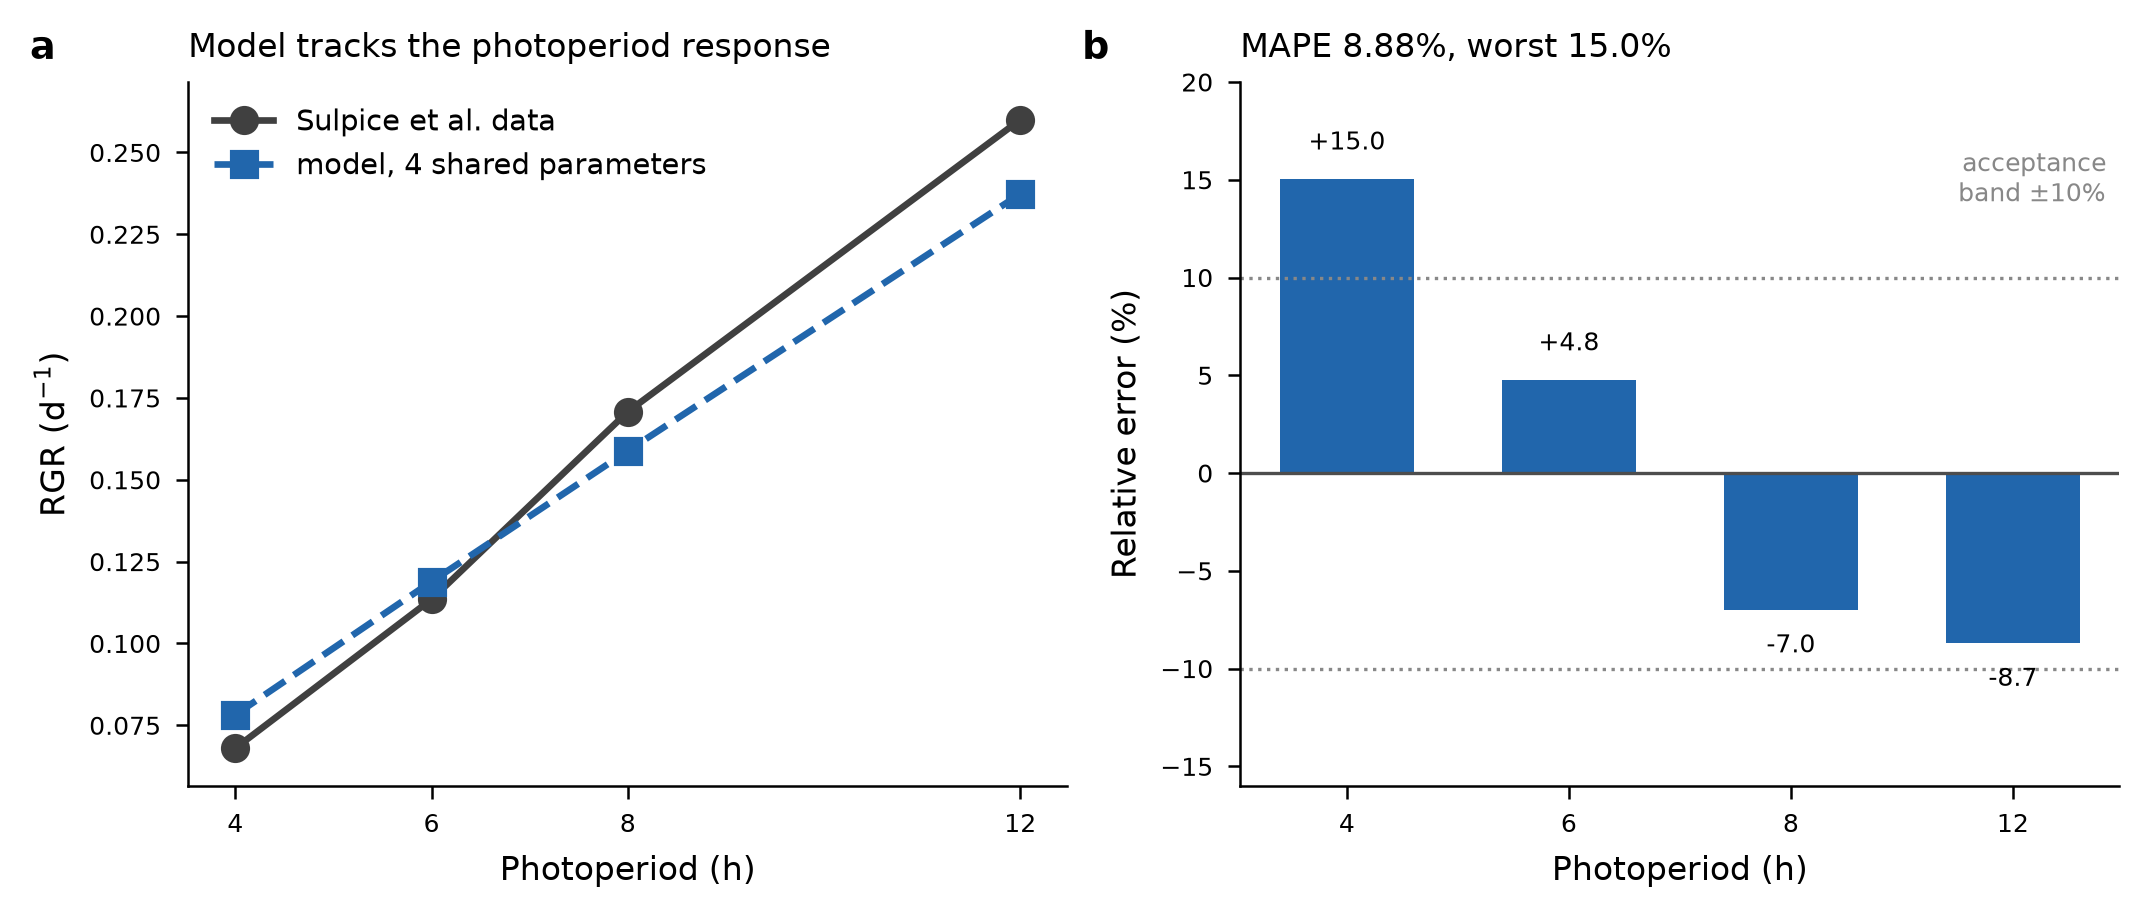
\includegraphics[width=\linewidth]{rgr_validation.png}
\caption{Relative growth rate against photoperiod. Simulated values under the
shared four-parameter parameterisation are compared with the reference targets
of \citet{Sulpice2014} for 4, 6, 8 and 12~h photoperiods. The residuals of the
saturated per-photoperiod calibration are shown for reference only; they are
convergence residuals of a fit with zero degrees of freedom.}
\label{fig:rgr}
\end{figure}

\subsection{Cross-photoperiod prediction}
\label{sec:results:crossval}

The held-out test asks a different question: how well does the model predict a
photoperiod that was not used to fit anything? We fitted the growth coefficient
on three photoperiods, predicted the fourth, and repeated this for each of the
four folds. Table~\ref{tab:crossval} reports both regimes and
Figure~\ref{fig:crossval} shows the predictions.

In regime A the growth coefficient is one shared constant. The held-out error is
$13.18\%$ and the worst fold is $20.93\%$, with the 4~h treatment held out. In
regime B the same coefficient depends linearly on photoperiod $P$,

\begin{equation}
\lambda_{sb}(P) = c_0 + c_1 P,
\label{eq:lsb_linear}
\end{equation}

with two coefficients instead of one. The held-out error falls to $4.36\%$ and
the worst fold is $10.30\%$, now at the 12~h treatment. The fitted values are
$c_0 = 0.00243$ and $c_1 = 8.786\times10^{-5}$ per hour. Across the four folds
the fitted growth coefficient rises monotonically with photoperiod, from
$0.00275$ at 4~h to $0.00370$ at 12~h. Adding one coefficient therefore
predicts an unseen photoperiod about three times better than a single
constant.

Two readings follow. First, the growth coefficient is not photoperiod-invariant
in this model. If the coupled dynamics generated the full photoperiod response,
a shared constant would be enough and regime B would add nothing. Second, the
missing dependence is compact. A straight line in one coefficient captures it
over the tested range, which places it in the conversion from available sucrose
to structural growth rather than in the gas-exchange layer upstream. A positive
slope means that a longer day converts loaded sucrose into biomass more
efficiently, not only for longer. Increased sink activity under long days is a
plausible reading \citep{Smith2007,Sulpice2014}, but the design cannot separate
it from an allocation effect or from a fresh-weight conversion effect.

The limits of Eq.~\ref{eq:lsb_linear} belong with the result. The line was
fitted over 4 to 12~h and has no support outside that interval. It corrects a
model coefficient and does not describe a process, so extrapolating it to 18 or
24~h has no basis. It must also break down at short photoperiods, because the
coefficient would reach zero at a positive day length.

\begin{table}[!htbp]
\centering
\caption{Leave-one-photoperiod-out prediction of relative growth rate. In
regime A the growth coefficient is a single shared constant; in regime B it is
linear in photoperiod with two coefficients (Eq.~\ref{eq:lsb_linear}). Train
error is the mean over the three fitted photoperiods; test error is the
held-out photoperiod. The $\lambda_{sb}$ column gives the value applied at the
held-out photoperiod.}
\label{tab:crossval}
\begin{tabular}{@{}llrrr@{}}
\toprule
Regime & Held out (h) & $\lambda_{sb}$ & Train MAPE (\%) & Test MAPE (\%) \\
\midrule
A: shared constant & 4  & 0.00320 & 5.57 & 20.93 \\
A: shared constant & 6  & 0.00320 & 9.24 &  9.94 \\
A: shared constant & 8  & 0.00295 & 8.08 & 10.10 \\
A: shared constant & 12 & 0.00295 & 7.53 & 11.75 \\
\midrule
\multicolumn{4}{@{}l}{Regime A, mean held-out error} & 13.18 \\
\midrule
B: linear in $P$ & 4  & 0.00275 & 2.25 &  3.42 \\
B: linear in $P$ & 6  & 0.00295 & 2.97 &  1.28 \\
B: linear in $P$ & 8  & 0.00320 & 2.57 &  2.45 \\
B: linear in $P$ & 12 & 0.00370 & 2.38 & 10.30 \\
\midrule
\multicolumn{4}{@{}l}{Regime B, mean held-out error} & 4.36 \\
\bottomrule
\end{tabular}
\end{table}

\begin{figure}[!htbp]
\centering
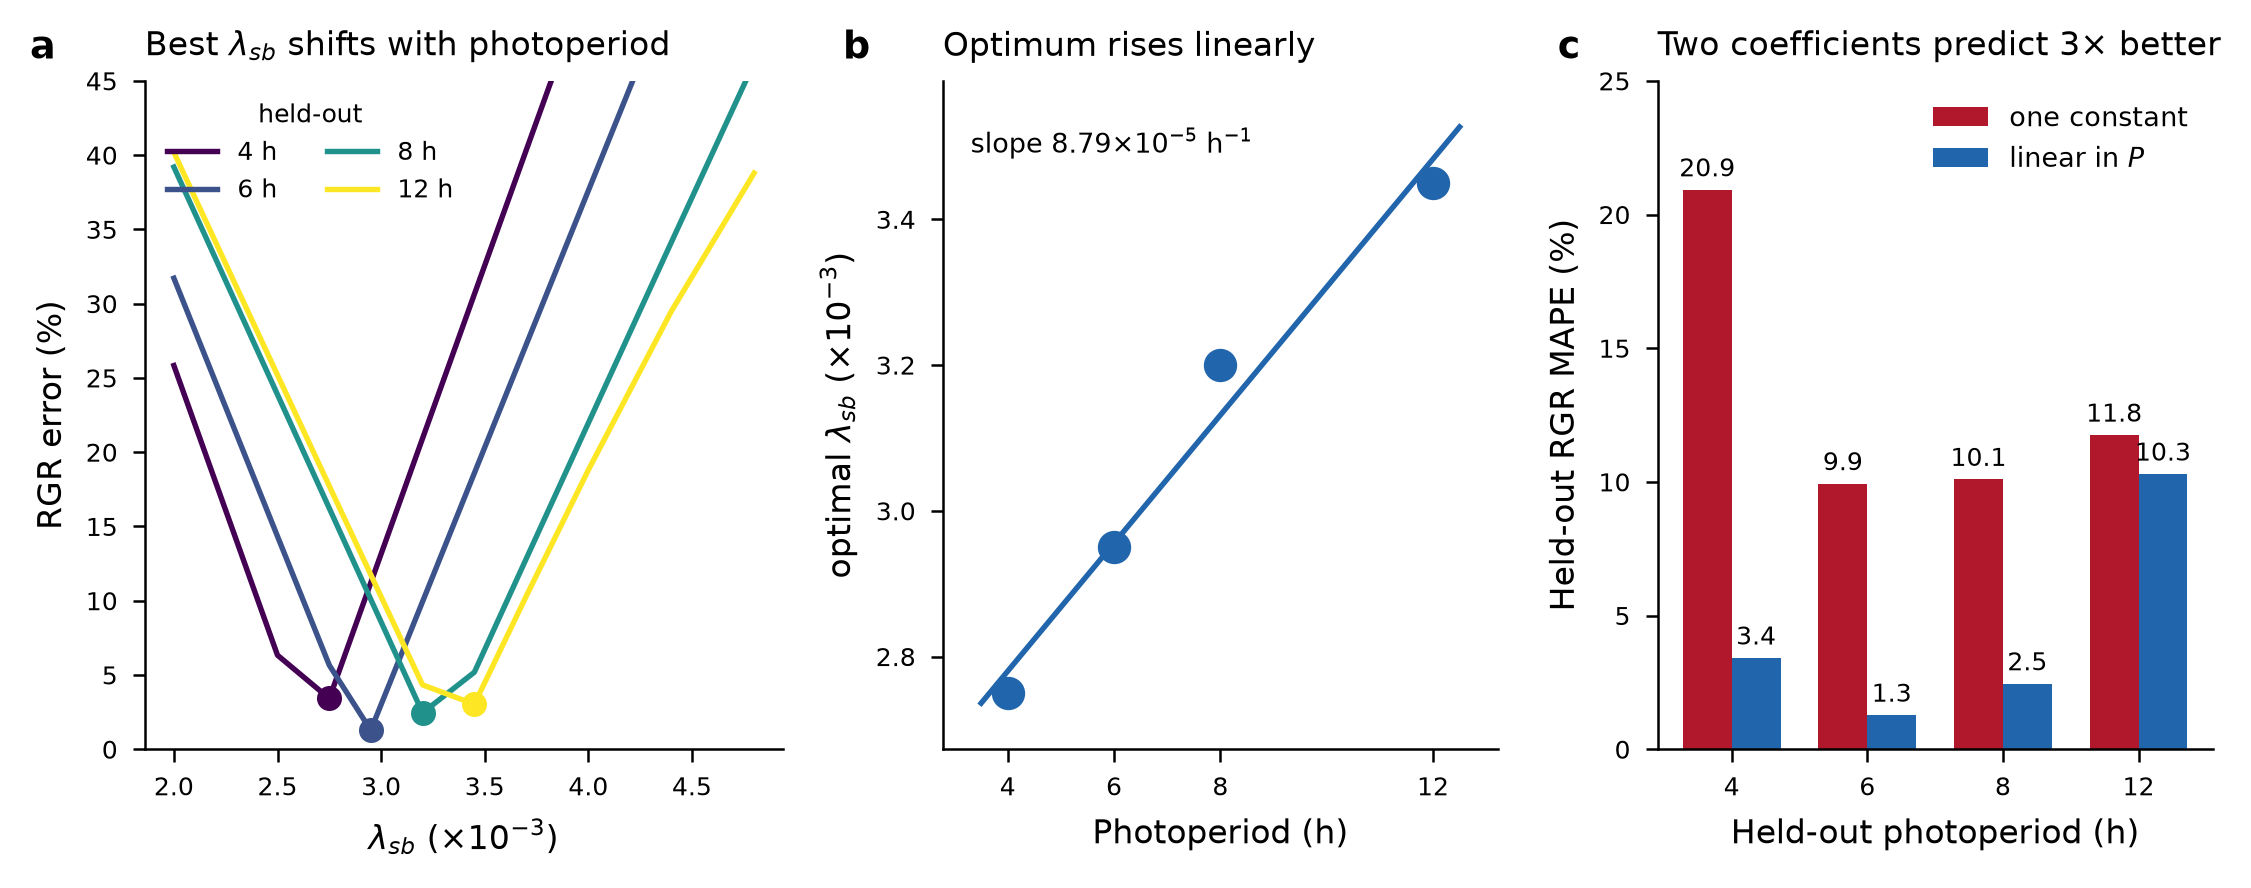
\includegraphics[width=\linewidth]{crossval.png}
\caption{Held-out photoperiod prediction of relative growth rate. Regime A
uses one shared growth coefficient; regime B lets the same coefficient vary
linearly with photoperiod (Eq.~\ref{eq:lsb_linear}). Each point is a
photoperiod that was excluded from the fit that produced it.}
\label{fig:crossval}
\end{figure}

\subsection{Diel carbohydrate dynamics}
\label{sec:results:carb}

The carbohydrate comparison uses one multiplicative scale per series, fitted
by least squares before the error is computed, so the normalised RMSE scores
the shape and the timing of the diel cycle. Over the reference series the mean
starch nRMSE is $0.235$ against the acceptance threshold of $0.25$, with a bias
of $-3.1\%$. The mean sucrose nRMSE is $0.285$ against a threshold of $0.50$,
with a bias of $+10.7\%$. In the validation runs the largest per-photoperiod
values are $0.219$ for starch and $0.468$ for sucrose. Figure~\ref{fig:carb}
shows the traces.

The two series are not equally strong, and the fitted scales show why. For
starch the scale is between $0.86$ and $1.15$ over the four fitted
photoperiods, so shape and absolute level both agree and the starch nRMSE
means what a reader would assume it means. For sucrose the scale is between
$2.25$ and $3.31$: the simulated pool must be multiplied by a factor of two to
three before it matches the measurements. Raw simulated sucrose maxima are
$1.30$ to $1.40~\mu\mathrm{mol}$ C$_6$ gFW$^{-1}$ against measured maxima of
$3.18$ to $4.71~\mu\mathrm{mol}$ C$_6$ gFW$^{-1}$. The passing sucrose nRMSE
of $0.285$ therefore describes shape and timing only, and the absolute sucrose
level is a known deficit of this version. We report the scale factor beside
every carbohydrate error for that reason.

Within the fitted range the model reproduces the qualitative features of the
diel cycle. Starch accumulates through the light period and degrades through the
night along a near-linear trajectory. At dawn it returns to the level at which
each run started, so the pool is close to empty at the end of every night. This
behaviour follows from the drain law of
Section~\ref{sec:carbohydrates}, which targets the remaining pool over the
remaining night, and it agrees with the near-linear nocturnal degradation
reported for \textit{Arabidopsis} \citep{Graf2010,Scialdone2013}.

One quantitative feature is not reproduced. The measured end-of-day starch
peak grows more steeply with photoperiod than the simulated peak. In the model
the peak does rise with photoperiod, because the light period is longer, but the
rise is weaker than measured. The model therefore under-represents how much a
long day changes the size of the transient store, as opposed to its filling
time. The same shortfall appears from the other side in
Section~\ref{sec:results:envelope}, where assimilation per light hour is found
to be constant.

\begin{figure}[!htbp]
\centering
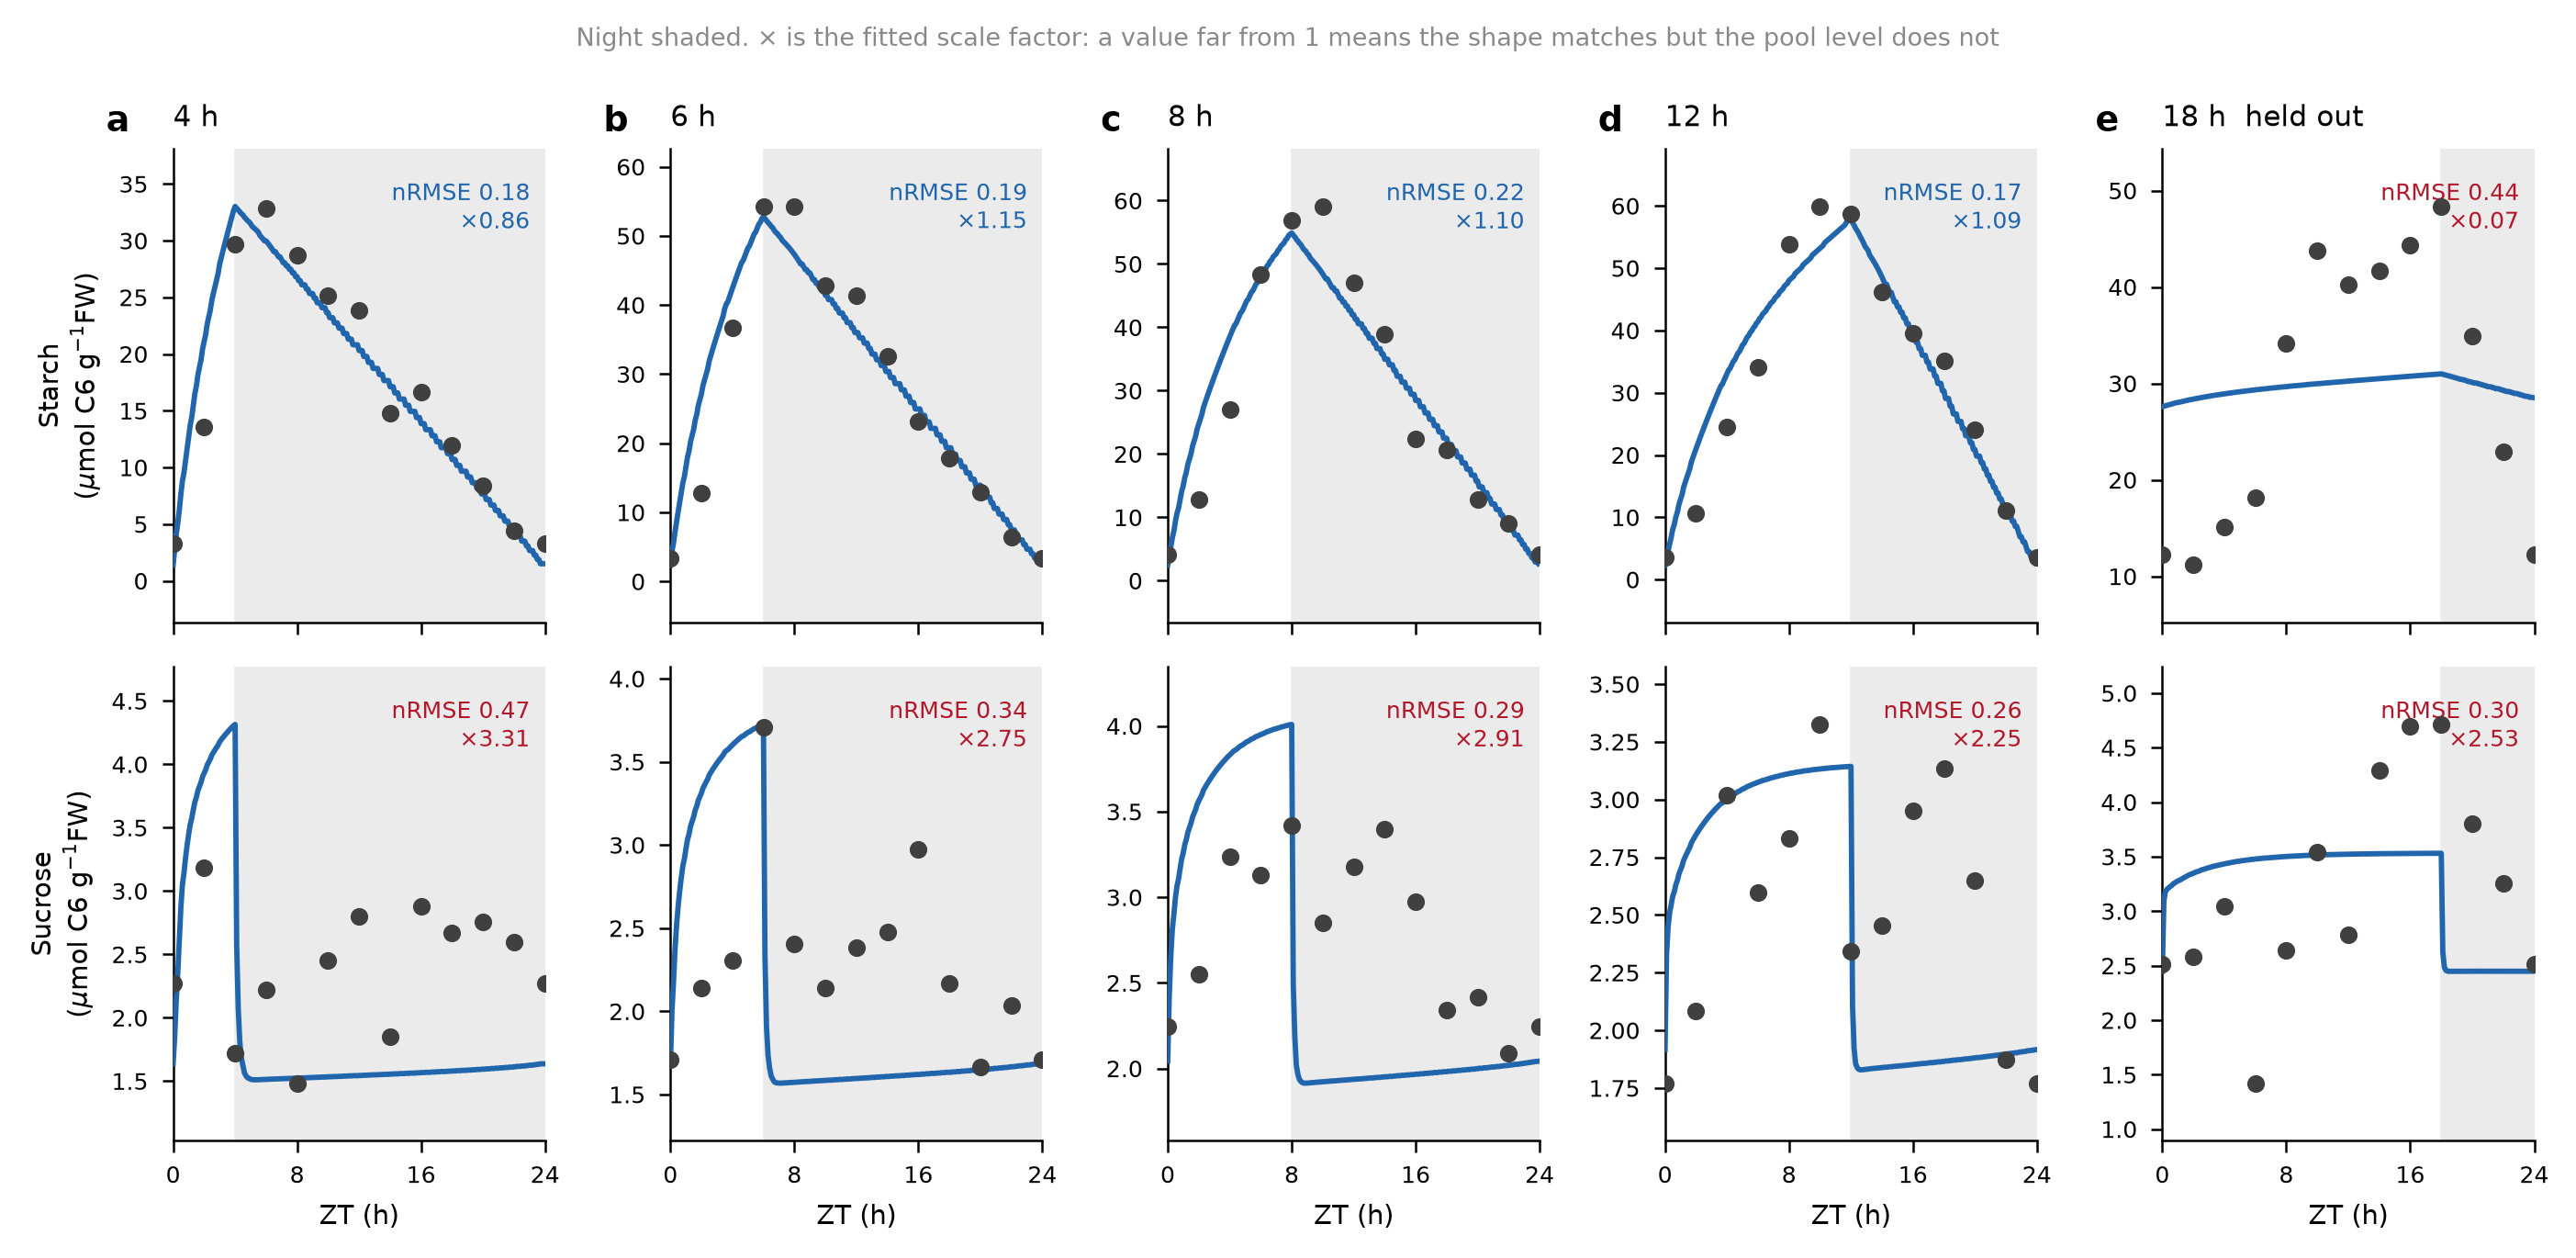
\includegraphics[width=\textwidth]{carbohydrate_diel.png}
\caption{Diel starch and sucrose dynamics for the 4, 6, 8, 12 and 18~h
photoperiods. Simulated traces are compared with the measured diel profiles of
the repository reference file (see Section~\ref{sec:protocol}). Each panel prints the nRMSE and
the fitted multiplicative scale. The scale is between $0.86$ and $1.15$ for
starch at the four fitted photoperiods and between $2.25$ and $3.31$ for
sucrose, so the sucrose comparison is one of shape and timing and not of
absolute level. The 18~h column was not used in any fit; its starch nRMSE is
not reported, because the fitted scale of $0.07$ absorbs the divergence
described in Section~\ref{sec:results:envelope}.}
\label{fig:carb}
\end{figure}

\subsection{Ablation}
\label{sec:results:ablation}

The ablation compares three carbon-input pathways with the same downstream
model, the same shared parameters and no refitting. In M0 the carbon input is
prescribed. In M1 it is computed from Farquhar photosynthesis
\citep{Farquhar1980} at fixed stomatal conductance. In M2 the conductance
follows the Jarvis formulation \citep{Jarvis1976} and responds to the
environment. Table~\ref{tab:ablation} and Figure~\ref{fig:ablation} give the
result: the RGR error falls from $41.01\%$ for M0 to $9.43\%$ for M1 and to
$8.88\%$ for M2.

The large step is from prescribed to computed carbon input. M0 underestimates
RGR at every photoperiod, by $39.2$ to $43.1\%$, and its peak assimilation
stays between $10.50$ and $11.14~\mu\mathrm{mol}$ gFW$^{-1}$ h$^{-1}$. With
computed assimilation the peak rises to $17.62$ and the systematic
underestimation disappears. The bias is not reduced but removed: M1 and M2
scatter on both sides of the targets, while M0 is low in all four scenarios.
Parameters were frozen across the three variants, so the change comes from the
carbon-input pathway and not from recalibration.

The Jarvis layer adds a smaller and unevenly distributed gain. Averaged over
the four photoperiods it reduces the error from $9.43$ to $8.88\%$, and the two
variants differ most at the extremes of the range. At 4~h, M2 improves on M1
by $3.8$ percentage points, from $18.82$ to $15.04\%$. At 12~h it is worse by
$2.1$ points, $8.71$ against $6.60\%$. At 6~h M2 is better by $3.0$ points and
at 8~h it is worse by $2.5$ points. Adding environmental control of conductance lowers peak
assimilation slightly, from $17.62$ to $17.01~\mu\mathrm{mol}$ gFW$^{-1}$
h$^{-1}$, because the conductance multipliers are below one at the nominal
condition. The value of M2 at a single nominal condition is therefore not a
gain in RGR accuracy. Its value is that the carbon input responds to
irradiance, humidity, temperature, ambient CO$_2$ and leaf water potential at
all, which is what the sensitivity analysis of the next subsection exercises.

\begin{table}[!htbp]
\centering
\caption{Ablation of the carbon-input pathway. M0 prescribes the carbon input,
M1 computes it from Farquhar photosynthesis at fixed conductance, and M2 adds
Jarvis stomatal conductance. Shared parameters are frozen across the three
variants. Errors are relative errors in RGR; the last column is the peak
assimilation rate.}
\label{tab:ablation}
\begin{tabular}{@{}lrrrrrr@{}}
\toprule
& \multicolumn{4}{c}{RGR error (\%) by photoperiod} & MAPE & Peak $\Phi_c$ \\
Variant & 4~h & 6~h & 8~h & 12~h & (\%) & ($\mu$mol gFW$^{-1}$h$^{-1}$) \\
\midrule
M0 prescribed        & 41.59 & 40.19 & 43.08 & 39.20 & 41.01 & 10.50--11.14 \\
M1 Farquhar          & 18.82 &  7.77 &  4.55 &  6.60 &  9.43 & 17.62 \\
M2 Farquhar--Jarvis  & 15.04 &  4.77 &  7.00 &  8.71 &  8.88 & 17.01 \\
\bottomrule
\end{tabular}
\end{table}

\begin{figure}[!htbp]
\centering
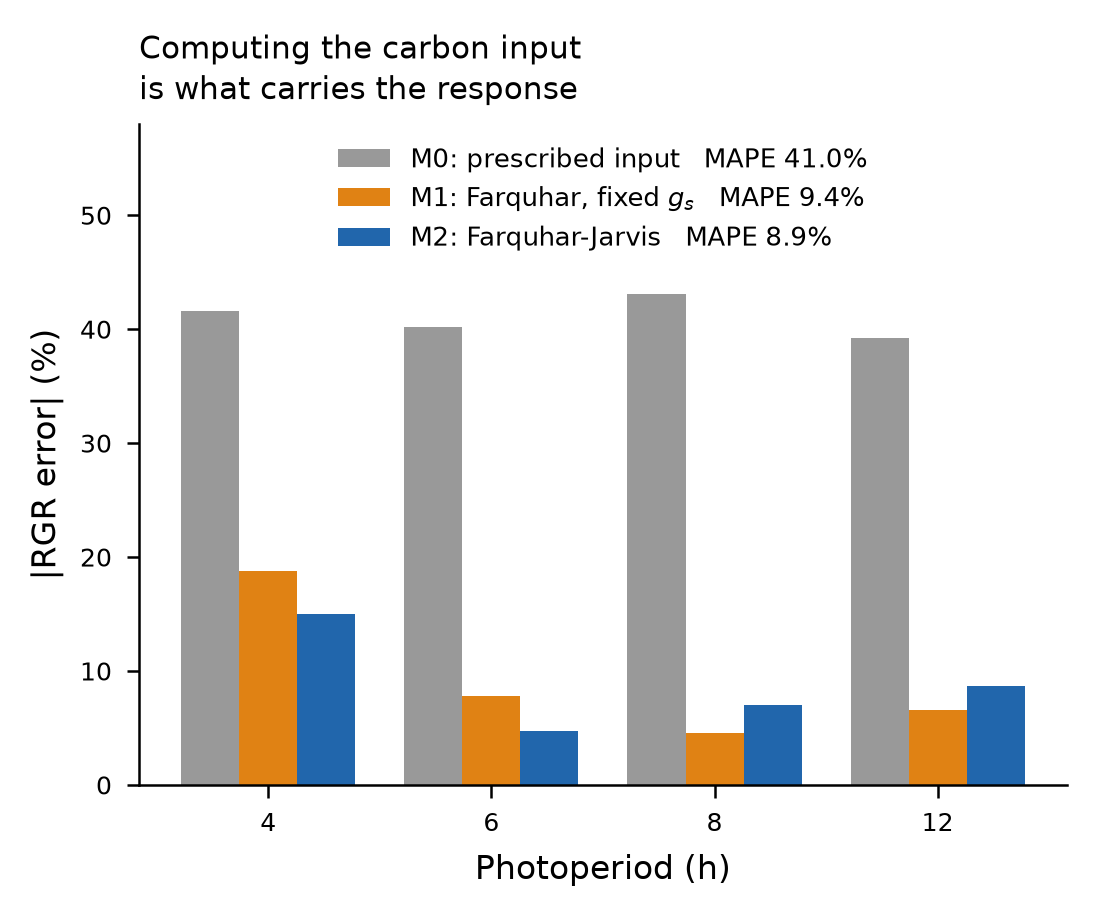
\includegraphics[width=0.58\linewidth]{ablation.png}
\caption{Relative RGR error per photoperiod for the three carbon-input
variants, with shared parameters frozen. M0 underestimates growth at every
photoperiod; M1 and M2 scatter on both sides of the targets.}
\label{fig:ablation}
\end{figure}

\subsection{Global sensitivity}
\label{sec:results:sens}

The variance-based analysis follows \citet{Sobol2001} with the estimator of
\citet{Saltelli2010}, and the Morris screening follows
\citet{Morris1991,Campolongo2007}. Sixteen parameters were varied over the
declared ranges of Appendix~\ref{app:sa}. Table~\ref{tab:sens} gives the full
ranking and Figure~\ref{fig:sens} shows the total-order indices next to the
Morris measures.

Nutrient uptake capacity dominates the total-order ranking. The two largest
total indices are $0.658$ for maximum phosphorus uptake and $0.577$ for maximum
nitrogen uptake. Respiration frequency follows at $0.466$, then ambient CO$_2$
concentration at $0.422$ and leaf water potential at $0.412$. The two Farquhar
capacities come next, $0.352$ for electron transport rate and $0.334$ for
maximum carboxylation rate, then maximum PAR at $0.333$. The ranking spans the
nutrient, respiratory and gas-exchange blocks, as expected in a model where
growth is limited by whichever supply is scarcest.

The main-effect share is small. Summed over the sixteen parameters and averaged
over the four photoperiods, the first-order indices give $0.201$ against a
summed total-order index of $4.675$, a main-effect share of about $4\%$. The
Morris measures agree: 15 of the 16 parameters have $\sigma/\mu^{*} > 1$, and
the exception is the one parameter with a total index at noise level. The two
methods also rank the parameters consistently, with a Spearman rank correlation
of $\rho = 0.944$ between Morris $\mu^{*}$ and Sobol' $S_T$. The model is
interaction-dominated over the declared ranges: parameters act mainly through
each other, not on their own.

A low main-effect share can also be an estimator artefact, so we checked
convergence with sample size. As $n$ rises from $512$ to $4096$, the number of
first-order estimates clipped at zero falls from $8$ to $3$. Over the same
range the summed first-order index stays between $0.151$ and $0.340$, and the
main-effect share stays between $3.0$ and $6.4\%$. The clipping decreases, which is what an
estimator with shrinking variance should do, but the share does not increase
with it. The low main-effect share is therefore a property of the model over
these ranges and not an artefact of a small sample. All indices in
Table~\ref{tab:sens} are reported unclipped, so small negative interaction
remainders appear where an index is at noise level; we prefer that to hiding
the estimator variance.

One entry deserves a comment. The growth coefficient $\lambda_{sb}$, the
coefficient that Section~\ref{sec:results:crossval} shows to carry the
photoperiod response, has a total index of only $0.117$ and ranks fifteenth of
sixteen. There is no contradiction. A Sobol' index measures the variance
contribution over a declared range at fixed forcing, while the
cross-photoperiod result measures how a coefficient must change when the
forcing changes. A parameter can be unimportant for variance at one condition
and still be the parameter that fails to transfer between conditions.

\begin{table}[!htbp]
\centering
\caption{Global sensitivity of relative growth rate, averaged over the four
photoperiods. $S_1$ is the first-order and $S_T$ the total-order Sobol' index;
the interaction remainder is $S_T - S_1$. $\mu^{*}$ and $\sigma$ are the
Morris measures. Indices are reported unclipped, so a remainder at noise level
can be slightly negative. Ranges and sampling scales are in
Appendix~\ref{app:sa}; the indices are conditional on those ranges.}
\label{tab:sens}
\footnotesize
\begin{tabular}{@{}lrrrrr@{}}
\toprule
Parameter & $S_1$ & $S_T$ & $S_T-S_1$ & $\mu^{*}$ & $\sigma/\mu^{*}$ \\
\midrule
\texttt{max\_phosphorus\_uptake}   & 0.000 & 0.658 & 0.658 & 0.635 & 1.73 \\
\texttt{max\_nitrogen\_uptake}     & 0.000 & 0.577 & 0.577 & 0.785 & 1.48 \\
\texttt{respiration\_frequency}    & 0.031 & 0.466 & 0.435 & 0.466 & 1.94 \\
\texttt{ambient\_CO2\_concentration} & 0.000 & 0.422 & 0.422 & 0.370 & 2.13 \\
\texttt{leaf\_water\_potential}    & 0.063 & 0.412 & 0.349 & 0.597 & 1.57 \\
\texttt{electron\_transport\_rate} & 0.020 & 0.352 & 0.332 & 0.247 & 2.57 \\
\texttt{max\_rubisco\_carboxylation\_rate} & 0.013 & 0.334 & 0.321 & 0.393 & 2.16 \\
\texttt{max\_PAR}                  & 0.000 & 0.333 & 0.333 & 0.463 & 1.96 \\
\texttt{leaf\_temperature}         & 0.008 & 0.219 & 0.211 & 0.198 & 3.05 \\
\texttt{relative\_humidity}        & 0.000 & 0.199 & 0.199 & 0.222 & 2.84 \\
\texttt{phosphorus\_soil\_content} & 0.017 & 0.164 & 0.148 & 0.202 & 2.62 \\
\texttt{sucrose} (initial)         & 0.007 & 0.144 & 0.137 & 0.164 & 2.70 \\
\texttt{nitrogen\_soil\_content}   & 0.007 & 0.141 & 0.134 & 0.100 & 3.72 \\
\texttt{k\_vacuole\_in}            & 0.009 & 0.135 & 0.126 & 0.101 & 3.96 \\
\texttt{lambda\_sb}                & 0.023 & 0.117 & 0.094 & 0.073 & 3.32 \\
\texttt{total\_biomass} (initial)  & 0.003 & 0.001 & $-0.002$ & 0.066 & 0.37 \\
\midrule
Sum & 0.201 & 4.675 & & & \\
\bottomrule
\end{tabular}
\end{table}

\begin{figure}[!htbp]
\centering
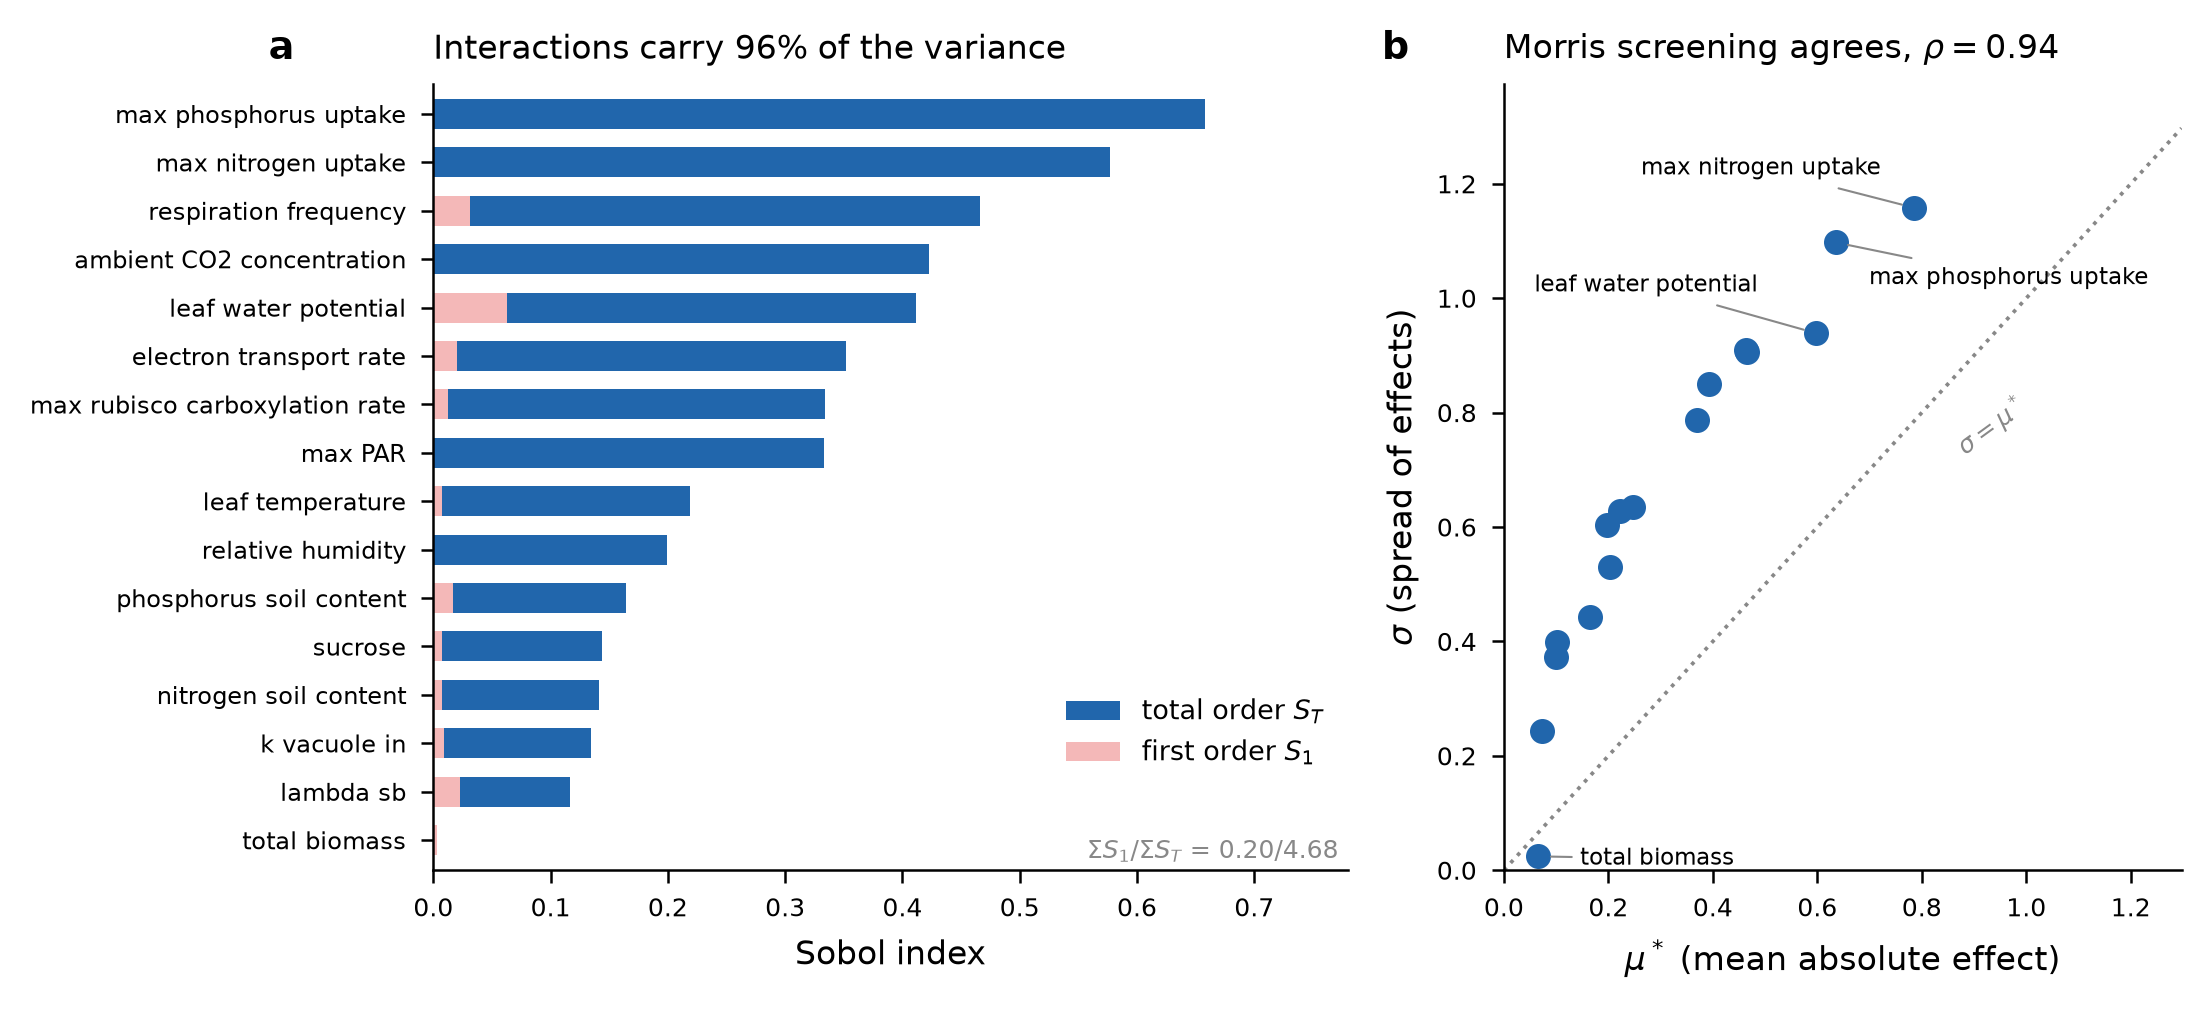
\includegraphics[width=\textwidth]{sensitivity.png}
\caption{Global sensitivity of relative growth rate over the declared
parameter ranges. Left: total-order Sobol' indices with the first-order part
shown separately. Right: Morris $\mu^{*}$ and $\sigma$. The two rankings agree
at a Spearman correlation of $0.944$, and 15 of the 16 parameters have
$\sigma/\mu^{*} > 1$.}
\label{fig:sens}
\end{figure}

\subsection{Validity envelope}
\label{sec:results:envelope}

Two limits of the model were measured directly, and we report them as findings
rather than as caveats. Figure~\ref{fig:envelope} shows both.

The first limit is the 18~h photoperiod, which was never used in any fit. The
sucrose comparison passes: nRMSE is $0.428$ against the threshold of $0.50$,
with a fitted scale of $2.53$, so the shape of the diel sucrose cycle survives
three hours beyond the fitted range. The starch pool does not. Dawn starch is
$401~\mu\mathrm{mol}$ gFW$^{-1}$ on day 30 and $1207~\mu\mathrm{mol}$ gFW$^{-1}$
on day 90, a net gain of about $+14$ per day that shows no sign of levelling
off. This is unbounded accumulation and not a wrong steady level, and the
distinction matters, because a wrong level can be rescaled while a divergence
cannot. The fitted scale for 18~h starch is $0.07$, which is the metric
absorbing the divergence, so no 18~h starch nRMSE is quoted anywhere in this
paper.

The mechanism is visible in the fluxes. The degradation cap is not binding at
18~h, so the failure is not a saturated drain. The drain law targets the
remaining pool over the remaining night, so nightly export is proportional to
what is left and to the reciprocal of the night length. Under a long day the
pool filled during the light period grows while the night available to empty it
shrinks. The day fill then outruns the drain, the pool carries a surplus into
the next day, and the surplus compounds.

The second limit is the closure boundary. Under the chamber forcing the net
daily starch gain is $+0.300$ at 12~h, $+0.295$ at 14~h and $+0.389$ at
15.0~h, rising to $+0.547$ at 15.5~h, $+2.042$ at 16~h, $+13.780$ at 18~h and
$+24.150$ at 20~h. The diel balance therefore closes up to $15.0$--$15.5$~h and
fails from 16~h. That boundary sits three hours beyond the longest photoperiod
used in any fit, which is a real margin and a narrow one.

The boundary is a property of the model and of the light dose together, not of
the model alone. Under the shipped half-sine profile at
$1200~\mu\mathrm{mol}$ m$^{-2}$ s$^{-1}$ the same measurement gives $+18.99$
at 12~h, $+32.56$ at 14~h, $+38.75$ at 15~h, $+45.00$ at 16~h, $+56.70$ at
18~h and $+67.68$ at 20~h. Under that dose the balance never closes, not even
at 12~h. Any statement of the form ``the model closes the diel starch balance
up to $P$ hours'' is therefore incomplete without the irradiance at which it
was measured. We report the chamber column as the envelope of this model, because it is the
condition with an experimental counterpart. The shipped column shows how
strongly the boundary depends on the daily photon dose.

The third measurement is a bound rather than a boundary, and it explains the
residual error of Section~\ref{sec:results:rgr}. Assimilation per hour of light
is constant to six significant figures across the photoperiod series, so total
daily assimilation is proportional to day length. The ratio of daily
assimilation between the 12 and 4~h scenarios is therefore exactly
$3.0000$, while the reference RGR targets require a ratio of $3.82$. Growth in
this model is driven by the carbon input, so a supra-proportional factor of
$1.27$ has to come from somewhere else. Partitioning cannot supply it: the
partition coefficients redistribute a fixed daily input between starch,
sucrose and biomass, and they cannot make the total larger. This is the same
gap that Eq.~\ref{eq:lsb_linear} closes empirically, seen at the level of the
carbon budget instead of the fitted coefficient.

\begin{figure}[!htbp]
\centering
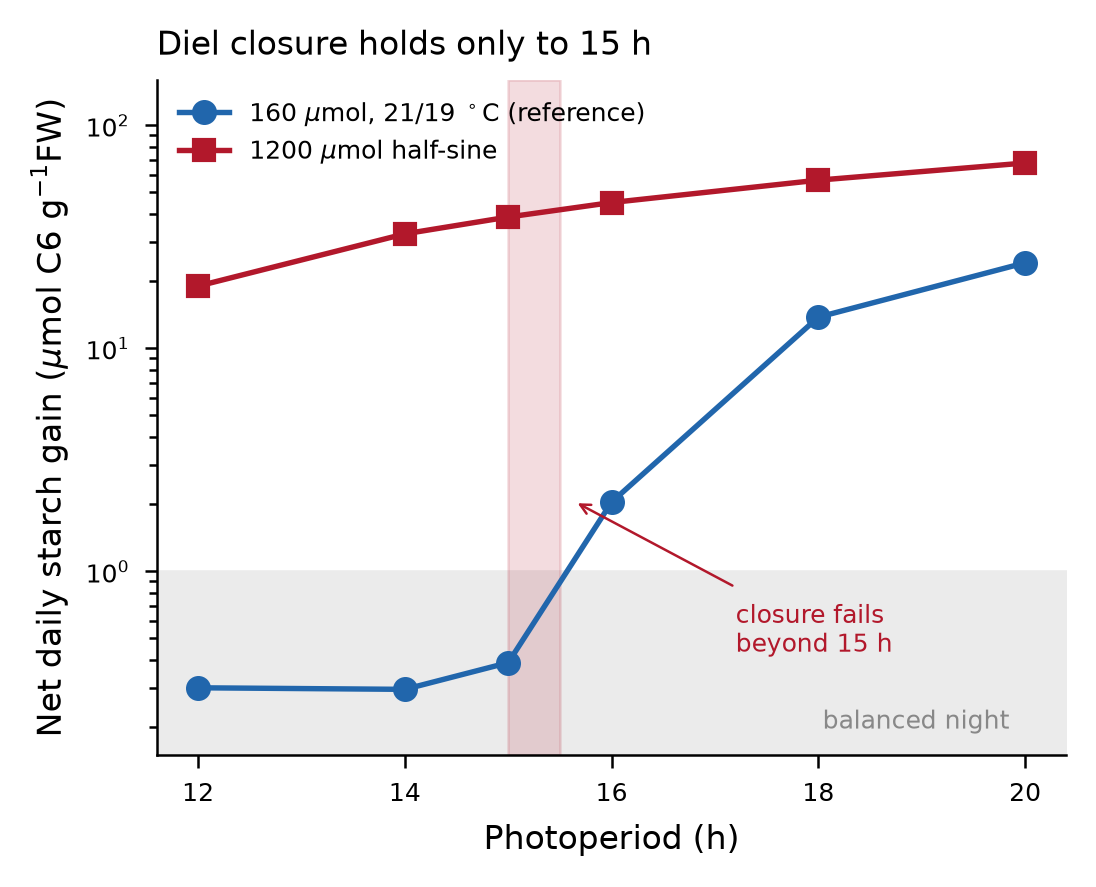
\includegraphics[width=0.58\linewidth]{validity_envelope.png}
\caption{Net daily starch gain against photoperiod on a symmetric-log axis,
under the chamber forcing and under the shipped half-sine profile at
$1200~\mu\mathrm{mol}$ m$^{-2}$ s$^{-1}$. The band marks the closure boundary
at $15.0$--$15.5$~h under chamber forcing. Under the higher dose the balance
does not close at any photoperiod shown, so the boundary depends on the light
dose as well as on the model.}
\label{fig:envelope}
\end{figure}

\section{Discussion}
\label{sec:discussion}

\subsection{What the coupled formulation buys}

The ablation puts a number on the coupling. Replacing a prescribed carbon input
with a computed one reduces the RGR error from $41.01$ to $9.43\%$ with no
parameter refitted. It removes a bias rather than reducing a scatter: M0 is low
at all four photoperiods, M1 and M2 are not. The reason is visible in the
assimilation rate. A prescribed maximum rate has to be chosen once, and a single
choice cannot be correct at four day lengths. The plant it describes has a
different leaf area and a different sucrose status in each case. The
computed input is a function of the states and of the forcing, so it changes
with them.

The Jarvis layer should be read differently. It reduces the mean error from
$9.43$ to $8.88\%$, which is a small change, and it moves the error in opposite
directions at the two ends of the photoperiod range. Reporting that as an
accuracy gain would misstate it. What the layer provides is a carbon input that
responds to irradiance, humidity, temperature, ambient CO$_2$ and leaf water
potential. The sensitivity analysis shows this is not a formality: ambient
CO$_2$ has a total-order index of $0.422$, leaf water potential $0.412$ and
maximum PAR $0.333$. In M1 those three parameters would move nothing through
the conductance path. A model intended for use across environments needs that
path even when it does not improve a single nominal-condition metric, and a
model evaluated only at its calibration point cannot show the difference.

This is where the model sits relative to existing families. It is not a
field-scale crop simulator, and it does not resolve architecture as a
functional-structural model does. It is a compact whole-plant core in which the
carbon input is computed from the environment and then propagated explicitly
into carbohydrate, nutrient and biomass states, with the numerical treatment and
the evaluation protocol stated. Many whole-plant and crop simulators prescribe
that input \citep{Holzworth2014,Jones2003,deWit2019}, and the ablation measures
what prescribing it costs in this setting. The physiological submodels are
inherited \citep{Farquhar1980,Jarvis1976,vonCaemmerer2000}; the coupling, the
analytic closure and the evaluation are what this paper contributes.

\subsection{Parameter transferability and what the design exposed}

The cross-photoperiod result is the part of this work with the widest reach
beyond plant modelling. One shared growth coefficient predicts a held-out
photoperiod with $13.18\%$ error; the same coefficient made linear in
photoperiod predicts it with $4.36\%$. Both regimes use the same equations, the
same states and the same solver. The difference is entirely in how one
coefficient is allowed to depend on a condition of the experiment.

That is a statement about parameter transferability, and it is a common failure
mode in simulation practice. A coefficient fitted at one operating condition is
usually reported as a property of the model, and it is then applied at other
conditions as if it were one. When it is not, the model appears to be
structurally wrong, because the error shows up in the state trajectories rather
than in the parameter. Our results separate the two cases. The gas-exchange
layer, the carbohydrate subsystem and the nutrient subsystem all transfer with
fixed coefficients across 4 to 12~h. One coefficient in the growth-conversion
term does not, and it needs one extra degree of freedom to do so.

The design is what made this visible. A random train-test split over all
available observations would have placed neighbouring photoperiods on both
sides of the split, and interpolation between them would have hidden the
dependence. Holding out an entire condition asks the question that matters for
a simulator: does the fitted model work at a condition it has never seen? We
suggest leave-one-condition-out evaluation as a default for models calibrated
across a treatment series. The reason is not that it is more severe. It is the
design that localises a transferability failure to a specific coefficient. A
single held-out error tells you the model missed. A
sweep of held-out folds, each with its own refitted coefficient, tells you
which coefficient moved and in which direction, and here it moved monotonically
with photoperiod.

Two properties of the design make it reusable outside this model. First, the
held-out condition must be a condition and not a random subset, because random
splitting lets neighbouring treatments substitute for each other. Second, one
coefficient at a time should be released. Regime B differs from regime A by a
single degree of freedom, so the improvement from $13.18$ to $4.36\%$ can be
attributed to that coefficient and to nothing else. Releasing several
coefficients at once would have produced a similar error reduction and located
nothing. Together the two properties turn a fit quality measurement into a
diagnostic that names a term in the model, which is what a modeller needs before
deciding whether to recalibrate or to reformulate.

The physiological reading must stay careful. A growth coefficient that rises
with day length means that the conversion from loaded sucrose to structural
biomass becomes more efficient as the photoperiod lengthens. Increased sink
activity under long days is a plausible candidate \citep{Smith2007,Sulpice2014},
and so is a change in the ratio of fresh weight to carbon, and so is a shift in
allocation between leaf and root. The present data cannot separate these, and
one linear coefficient fitted over four photoperiods will fit all three
explanations equally well. We therefore report the dependence as a measured
property of the calibration and not as an identified mechanism.

\subsection{What the carbohydrate results do and do not show}

The two carbohydrate series should be read with different confidence. For starch
the fitted scales lie between $0.86$ and $1.15$, so the comparison covers level
as well as shape. A mean nRMSE of $0.235$ against a threshold of $0.25$ can
therefore be taken at face value. For sucrose the scales lie between $2.25$ and $3.31$, so
the same style of statement would be misleading. The passing value of $0.285$
means that the model puts the sucrose maxima and minima at the right times, with
roughly the right relative depth. It says nothing about the absolute pool size,
which is a factor of two to three too low.

The distinction matters beyond this model, because a scale-fitted error metric
is common when reference data are indirect or on a different basis. Fitting one
multiplicative scale is defensible: it separates a units or basis mismatch from a
dynamic error, and it is the only way to compare a normalised model pool against
a measured tissue concentration. But the fitted scale is part of the result and
must be reported with it. A scale near one and a scale near three support
different claims from the same nRMSE, and only the first supports a statement
about level.

\subsection{Interaction dominance and its consequences for calibration}

Over the declared parameter ranges, the summed first-order indices account for
about $4\%$ of the summed total-order indices. In addition, 15 of the 16
parameters have a Morris $\sigma/\mu^{*}$ above one. Two independent methods
agree on the ranking at $\rho = 0.944$, and the convergence check shows the low
main-effect share is stable as the sample grows. The
conclusion is not that main effects are absent, but that they are small
relative to interactions across the tested domain.

This has a practical consequence for anyone calibrating a model of this class.
One-at-a-time tuning is unreliable here. Suppose a parameter's own effect explains a few percent of the variance and the
rest comes from its interactions. The sensitivity measured by moving that
parameter alone then depends on where the other fifteen happen to sit. Tuning it at one operating point can make behaviour
worse at another, and the sequence in which parameters are tuned changes the
result. The structure of the model explains why. Growth is limited by whichever
supply is scarcest, and the largest total-order indices belong to the nutrient
uptake capacities, $0.658$ and $0.577$. A nutrient parameter changes which
limitation binds, and that changes how strongly every gas-exchange parameter
matters. The interaction is the model working as designed, and it means
calibration should be done jointly, with a global method, over a declared
domain.

Two limits on this reading should be kept. The indices are conditional on the
ranges in Appendix~\ref{app:sa}; wider ranges would raise the interaction share
and narrower ones would lower it. And they describe model behaviour, not plant
physiology. That nutrient uptake capacity dominates variance in this model is a
statement about this model over these ranges.

\subsection{Limitations}
\label{sec:limitations}

Six limitations bound what can be concluded, and each is measured rather than
asserted.

Four coefficients were fitted. The growth coefficient, the two starch
partitioning rates and the half-activation constant of the sink term were
estimated against the reference data, so the in-sample results of
Section~\ref{sec:results:rgr} are not independent tests. This is a large
improvement on the eight-per-photoperiod calibration of the earlier version,
which had zero degrees of freedom against eight observations, but four fitted
coefficients are still four. The held-out results of
Section~\ref{sec:results:crossval} and the 18~h evaluation of
Section~\ref{sec:results:envelope} are the parts of the evaluation that no
fitting touched.

The carbohydrate metric is scale-fitted, and for sucrose the fitted scale is
large. The starch scales lie between $0.86$ and $1.15$, so the starch
comparison covers level as well as shape. The sucrose scales lie between $2.25$
and $3.31$, so the simulated pool is a factor of two to three below the
measurements in absolute terms and the passing nRMSE of $0.285$ evaluates shape
and timing only. Raw simulated maxima are $1.30$ to $1.40~\mu\mathrm{mol}$
C$_6$ gFW$^{-1}$ against measured maxima of $3.18$ to
$4.71~\mu\mathrm{mol}$ C$_6$ gFW$^{-1}$. The deficit is one of the clearest
targets for the next version. It should also be read together with the
whole-tissue basis of the measurements. The model quantity compared here is the
sum of the cytosolic and vacuolar pools, so a partition error between the two
would not show in the total.

Some parameters remain unsourced. The provenance ledger classifies 12 of 111
entries as having no traceable origin and 15 as fitted, and both groups are
listed in Appendix~\ref{app:params} with that status attached. Unsourced
constants are a work list and not a defence; we report them so that a reader
can see which numbers rest on a measurement and which do not.

The diel starch balance closes only to $15.0$--$15.5$~h under chamber forcing,
and under the higher shipped light dose it does not close at any photoperiod
tested. The model is therefore not valid for long-day simulation as it stands,
and any application beyond the closure boundary would need the drain law
changed first.

The RGR response to photoperiod is bounded by construction. Assimilation per
light hour is constant to six significant figures, so daily assimilation is
proportional to day length, and the 12 to 4~h ratio is exactly $3.0000$ where
the targets need $3.82$. No choice of partitioning parameters can produce the
missing factor of $1.27$, because partitioning redistributes a fixed daily
input. The linear growth coefficient covers this gap empirically, and the
underlying bound remains.

Simulated tissue nutrient concentration falls with increasing supply where the
measurements rise. The nutrient block is out of sample, no coefficient in it
was fitted to the nutrient response, so it is entitled to judge the model and
the discrepancy is reported and not tuned away. The likely cause is in the
structure of the nutrient balance rather than in a parameter value. Every term in
the internal nutrient equation is bounded, and the concentration is consumed in
proportion to assimilation. A supply increase raises assimilation,
which raises consumption, and with a bounded uptake term the pool can fall.
Resolving this requires the uptake and consumption terms to be reformulated,
which is beyond a recalibration.

\subsection{Pushing the envelope past 15.5 hours}

The closure failure has a specific cause, so the candidate remedies are also
specific. The nocturnal drain targets the remaining pool over the remaining
night. Its rate therefore scales with the reciprocal of night length, while the
daytime fill scales with day length, and beyond about 15~h the fill wins. Three
changes could plausibly move the boundary, and each is testable within the
present model.

The first is to make the daytime partition to starch respond to the size of the
starch pool relative to what the coming night can export. In the current
formulation the partition coefficient responds to sucrose status, not to the
starch balance, so nothing tells the plant to stop filling a store it cannot
empty. Measurements support such a dependence, since \textit{Arabidopsis}
adjusts partitioning to starch across photoperiods
\citep{Sulpice2014,Mengin2017}. The second is to raise the degradation
capacity. The cap is not binding at 18~h, so it cannot be the limit on its own.
A higher cap combined with a drain law that also depends on the pool level would
extend the range over which the drain can match the fill. The third
is to allow the peak amplitude of the store to grow with photoperiod, which is
also the feature that Section~\ref{sec:results:carb} identifies as
under-represented against the measurements. That the same shortfall shows up in
the diel comparison and at the closure boundary suggests one structural cause
rather than two.

We do not claim any of these will work. Each adds a coefficient that would have
to be identified against data, and the measurements available at 18~h are
limited. A change that closes the balance could easily be a change that fits one
series. What we can state is narrower. The boundary sits at $15.0$--$15.5$~h under
chamber forcing, and its cause lies in the drain law and its interaction with
the day fill. Testing the three candidates above is the next step, not a
result.

\section{Conclusion}
\label{sec:conclusion}

We presented a whole-plant simulation model in which environmental forcing is
converted into a photosynthetic carbon input through Jarvis stomatal conductance
and Farquhar C3 photosynthesis. That carbon input is then propagated through
diel carbohydrate, nutrient and biomass dynamics. The supply and demand
sides of gas exchange are closed analytically at runtime as a quadratic in the
intercellular CO$_2$ concentration, so the operating point is obtained without
an inner iteration. The eleven slow states are advanced by an adaptive
integrator. The formulation, its numerical treatment and the evaluation
protocol are the contribution; the physiological submodels are inherited.

The evaluation used four shared fitted coefficients rather than the
eight-per-photoperiod calibration of the earlier version. In sample the model
reproduces the relative growth rate across four photoperiods with a mean
absolute percentage error of $8.58\%$. In a leave-one-photoperiod-out test, one
shared growth coefficient predicts a held-out photoperiod less well than the
same coefficient made linear in photoperiod, which reaches $4.36\%$ with two
coefficients. The ablation shows what the coupling contributes: replacing a
prescribed carbon input with a computed one moves the error from $41.01$ to
$8.88\%$ with parameters frozen. The variance-based analysis shows an
interaction-dominated model over the declared ranges, led by nutrient uptake
capacity, respiration and gas-exchange capacity. Calibration of this class of
model should therefore be done jointly, not one parameter at a time.

The paper also states where the model stops working. Under the chamber forcing the diel
starch balance closes up to a photoperiod of $15.0$ to $15.5$~h and fails
beyond it. Under a higher light dose it does not close at all, so the boundary
belongs to the model and the light dose together. At 18~h the sucrose
cycle still has the right shape while the starch pool accumulates without
bound. Assimilation per light hour is constant, which bounds the growth
response to photoperiod below what the reference data require, and the linear
growth coefficient covers that gap empirically rather than mechanistically. The
absolute sucrose level is a factor of two to three too low, so the sucrose
comparison is one of shape and timing.

Three directions follow. The drain law and the daytime partition to starch are
the place to look for a formulation that closes the balance at long days.
The absolute sucrose level and the nutrient concentration response are two
independent out-of-sample discrepancies that point at the structure of the
sucrose and nutrient balances rather than at their coefficients. And the
leave-one-condition-out design used here can be applied to other conditions,
irradiance and temperature first, to test whether the remaining coefficients
transfer as well across those as they do across photoperiod.

\appendix

\section{Parameter provenance ledger}
\label{app:params}

Every numerical constant in the released model carries a provenance record in
\texttt{config/parameter\_provenance.csv}, and Table~\ref{tab:provenance} is
generated from that file rather than transcribed. The tier states how the value
was obtained: T1 measured, T2 derived, T3 inherited, T4 constrained, T5 fitted, T6 unsourced. A T6 entry is a value that
we could not trace to a measurement, a derivation or the source model, and it is
declared as such rather than presented as sourced. The ledger holds 111 entries,
of which 2 are measured (T1), 52 are derived (T2), 20 are inherited (T3), 10 are constrained (T4), 15 are fitted (T5), 12 are unsourced (T6).

\begin{table*}[!htbp]
\centering
\tiny
\caption{Complete parameter provenance ledger, generated from
\texttt{config/parameter\_provenance.csv}. Locator gives the equation, section or
source line from which the value comes; a dash means no locator is recorded.}
\label{tab:provenance}
\begin{tabular}{@{}p{52mm}rp{20mm}cp{20mm}p{38mm}@{}}
\toprule
Parameter & Value & Unit & Tier & Source & Locator \\
\midrule
\texttt{gas\_exchange.specific\_leaf\_area} & 0.025 & m2 gDW-1 & T1 & ArabidopsisLeafAtlas2024 & Table 1, 'Leaf area per unit leaf fresh weight' = 5500 mm2/g LFW; Col-0 leaf 6 at 21 DAI \\
\texttt{photo.photoperiod} & 8 & h & T1 & Sulpice2014 & Methods / Supplemental Table 1 (4, 6, 8, 12 h treatments) \\
\texttt{carbohydrates.k\_vacuole\_out} & 0.041959 & h-1 & T2 & Seydel2025 & Plant Physiol 198:kiaf117, Suppl. Table S5 sheet ST3, control rows, n=5 \\
\texttt{carbohydrates.night\_efficiency\_starch} & 0.5 & - & T2 & -- & input.c:31; default.config:30 \\
\texttt{carbohydrates.starch} & 0.225 & umolC6/gFW & T2 & -- & input.c:42; default.config:41 \\
\texttt{carbohydrates.starch\_degradation\_rate} & 0 &  & T2 & -- & -- \\
\texttt{carbohydrates.starch\_night\_start} & 2 & umolC6/gFW & T2 & -- & -- \\
\texttt{carbohydrates.starch\_partition\_coeff} & 0.6 & - & T2 & -- & input.c:25; default.config:24 \\
\texttt{carbohydrates.sucrose} & 1.95 & umolC6/gFW & T2 & -- & input.c:41; default.config:40 \\
\texttt{carbohydrates.transport\_cost} & 0 &  & T2 & -- & -- \\
\texttt{carbohydrates.uptake\_cost} & 0 & umol C6 gFW-1 h-1 & T2 & Tedone2020 & \S 2.2.8 (n\_c*U\_N + p\_c*U\_P); config entry is a slot \\
\texttt{gas\_exchange.convert\_to\_photosynthesis\_per\_gram\_per\_hour} & 24000 & dimensionless & T2 & -- & -- \\
\texttt{gas\_exchange.light\_limited\_photosynthesis} & 10 &  & T2 & -- & -- \\
\texttt{gas\_exchange.light\_limited\_rate} & 10 &  & T2 & -- & -- \\
\texttt{gas\_exchange.net\_photosynthesis} & 10 &  & T2 & -- & -- \\
\texttt{gas\_exchange.net\_photosynthesis\_rate} & 10 &  & T2 & -- & -- \\
\texttt{gas\_exchange.respiration\_rate} & 1.5 &  & T2 & -- & -- \\
\texttt{gas\_exchange.rubisco\_limited\_photosynthesis} & 12 &  & T2 & -- & -- \\
\texttt{gas\_exchange.rubisco\_limited\_rate} & 12 &  & T2 & -- & -- \\
\texttt{growth.leaf\_biomass} & 0.02 & gFW & T2 & -- & input.c:14; default.config:15 \\
\texttt{growth.root\_biomass} & 0.02 & gFW & T2 & -- & input.c:15; default.config:16 \\
\texttt{growth.sucrose\_root\_allocation} & 0.5 & - & T2 & -- & input.c:86; default.config:74 \\
\texttt{growth.total\_biomass} & 0.04 & gFW & T2 & -- & input.c:16; default.config:17 \\
\texttt{hardcoded.photosynthesis.ref\_specific\_leaf\_area} & 0.025 & m2 gFW-1 & T2 & -- & -- \\
\texttt{nutrients.assimilation\_cost\_nitrogen} & 0.0460308 & umolN/umolC6 & T2 & Tedone2020 & Eq 2.2.16, Appendix A \\
\texttt{nutrients.assimilation\_cost\_phosphorus} & 0.00460308 & umolP/umolC6 & T2 & Tedone2020 & c\_sp = c\_sn/O, Appendix A (O = 10 umolN/umolP) \\
\texttt{nutrients.max\_nitrogen} & 23 & umolN/gFW & T2 & Tedone2020 & Eq 2.2.25 (n\_max = D*n\_min, D = 4) \\
\texttt{nutrients.max\_phosphorus} & 2.3 & umolP/gFW & T2 & Tedone2020 & after Eq 2.2.25 ("p\_max = n\_max / O") with O = 10 from Eq 2.2.7 \\
\texttt{nutrients.min\_nitrogen} & 5.75 & umolN/gFW & T2 & Tedone2020 & Eq 2.2.25 \\
\texttt{nutrients.min\_phosphorus} & 0.575 & umolP/gFW & T2 & Tedone2020 & after Eq 2.2.25 ("p\_max = n\_max / O") with O = 10 from Eq 2.2.7 \\
\texttt{nutrients.min\_phosphorus\_photosynthesis} & 0.575 & umolP/gFW & T2 & Tedone2020 & after Eq 2.2.25 ("p\_max = n\_max / O") with O = 10 from Eq 2.2.7 \\
\texttt{nutrients.nitrogen} & 8.625 & umolN/gFW & T2 & -- & input.c:43; default.config:42 \\
\texttt{nutrients.nitrogen\_affinity} & 0.5 &  & T2 & -- & -- \\
\texttt{nutrients.nitrogen\_cost} & 0 &  & T2 & -- & -- \\
\texttt{nutrients.nitrogen\_nutrient\_uptake} & 0 &  & T2 & -- & -- \\
\texttt{nutrients.nitrogen\_uptake} & 0 &  & T2 & -- & -- \\
\texttt{nutrients.phosphorus} & 0.8625 & umolP/gFW & T2 & -- & input.c:44; default.config:43 \\
\texttt{nutrients.phosphorus\_affinity} & 0.5 &  & T2 & -- & -- \\
\texttt{nutrients.phosphorus\_cost} & 0 &  & T2 & -- & -- \\
\texttt{nutrients.phosphorus\_nutrient\_uptake} & 0 &  & T2 & -- & -- \\
\texttt{nutrients.phosphorus\_uptake} & 0 &  & T2 & -- & -- \\
\texttt{nutrients.pot\_nitrogen\_uptake} & 0 &  & T2 & -- & -- \\
\texttt{nutrients.pot\_phosphorus\_uptake} & 0 &  & T2 & -- & -- \\
\texttt{nutrients.stoichiometric\_signal} & 0.5 & - & T2 & -- & input.c:87; default.config:75 \\
\texttt{photo.light} & 0 &  & T2 & -- & -- \\
\texttt{photo.limitation\_of\_photosynthetic\_rate} & 0.5 &  & T2 & -- & -- \\
\texttt{photo.nitrogen\_saturation} & 0.45 &  & T2 & -- & -- \\
\texttt{photo.phosphorus\_saturation} & 0.45 &  & T2 & -- & -- \\
\texttt{simulation.days} & 35 &  & T2 & -- & -- \\
\texttt{simulation.dt\_hours} & 0.1 &  & T2 & -- & -- \\
\texttt{simulation.gui\_enabled} & true &  & T2 & -- & -- \\
\texttt{simulation.solver\_tolerance} & 1e-08 &  & T2 & -- & -- \\
\texttt{simulation.solver\_type} & ODE45 &  & T2 & -- & -- \\
\texttt{simulation.write\_csv} & true &  & T2 & -- & -- \\
\texttt{carbohydrates.max\_starch\_degradation\_rate} & 6 & umolC6/(gFW h) & T3 & Tedone2020 & \S 2.2.4 \\
\texttt{carbohydrates.max\_sucrose} & 2 & umolC6/gFW & T3 & Tedone2020 & \S 2.2.4 (Eq 2.2.28) \\
\texttt{carbohydrates.min\_starch} & 0.15 & umolC6/gFW & T3 & Tedone2020 & \S 2.2.4 \\
\texttt{carbohydrates.min\_sucrose} & 1.3 & umolC6/gFW & T3 & Tedone2020 & \S 2.2.4 \\
\texttt{carbohydrates.respiration\_frequency} & 0.79 & 1/h & T3 & Tedone2020 & Section 2.2.8 (Costs), "r\_m\_bar = 0.79 1/h" \\
\texttt{carbohydrates.sucrose\_loading\_frequency} & 1.98 & 1/h & T3 & Tedone2020 & \S 2.2.8 (Eq 2.2.28) \\
\texttt{growth.leaf\_competitive\_rate} & 5e-06 & 1/(h gFW) & T3 & Tedone2020 & \S 2.2.10 (paragraph after Eq 2.2.33): "fixed to the small value 5e-6" \\
\texttt{growth.leaf\_deathrate} & 5e-06 & 1/h & T3 & Tedone2020 & \S 2.2.10 (paragraph after Eq 2.2.33): "fixed to the small value 5e-6" \\
\texttt{growth.root\_competitive\_rate} & 5e-06 & 1/(h gFW) & T3 & Tedone2020 & \S 2.2.10 (paragraph after Eq 2.2.33): "fixed to the small value 5e-6" \\
\texttt{growth.root\_deathrate} & 5e-06 & 1/h & T3 & Tedone2020 & \S 2.2.10 (paragraph after Eq 2.2.33): "fixed to the small value 5e-6" \\
\texttt{nutrients.Michaelis\_Menten\_constant\_nitrogen} & 0.125 & umolN cm-3 & T3 & Tedone2020 & \S 2.2.7 (Eq 2.2.22), "k\_n = 0.125 umolN/cm3" \\
\texttt{nutrients.Michaelis\_Menten\_constant\_phosphorus} & 0.006736 & umolP cm-3 & T3 & Tedone2020 & \S 2.2.7 (Eq 2.2.22), "k\_p = 0.006736 umolP/cm3" \\
\texttt{nutrients.max\_nitrogen\_uptake} & 6.44 & umolN/(gFW h) & T3 & Tedone2020 & \S 2.2.7 \\
\texttt{nutrients.max\_phosphorus\_uptake} & 0.4 & umolP/(gFW h) & T3 & Tedone2020 & \S 2.2.7 \\
\texttt{nutrients.min\_nitrogen\_photosynthesis} & 5.75 & umolN/gFW & T3 & Tedone2020 & Eq 2.2.5 \\
\texttt{nutrients.nitrogen\_uptake\_sucrose\_consumption} & 0.68 & umolC6/umolN & T3 & Tedone2020 & \S 2.2.8 \\
\texttt{nutrients.optimal\_stoichiometric\_ratio} & 10 & umolN/umolP & T3 & Tedone2020 & Eq 2.2.7, Eq 2.2.31 \\
\texttt{nutrients.phosphorus\_soil\_content} & 0.15 & umolP cm-3 & T3 & Tedone2020 & Appendix A [159] \\
\texttt{nutrients.phosphorus\_uptake\_sucrose\_consumption} & 0.308 & umolC6/umolP & T3 & Tedone2020 & \S 2.2.8 \\
\texttt{photo.max\_photosynthetic\_rate} & 12.7 & umolC6/(gFW h) & T3 & Tedone2020 & Eq 2.2.1, \S 2.2.2 \\
\texttt{DEFECT.algebraic.uptake\_cost\_evaluation\_order} & nan &  & T4 & conservation & src/model/algebraic.c:86 (call) vs :127/:131 (assignments) \\
\texttt{DEFECT.growth.no\_carbon\_price\_on\_biomass} & nan &  & T4 & conservation & src/model/carbohydrates.c:106 (sucrose\_production) vs src/model/growth.c:12 (leaf\_growth) \\
\texttt{carbohydrates.sucrose\_consumption\_transport} & 0.035 & - & T4 & Tedone2020 & Appendix A (0.0035) vs body text 2.2.8 (0.035) \\
\texttt{gas\_exchange.ambient\_CO2\_concentration} & 400 & umol mol-1 & T4 & -- & -- \\
\texttt{gas\_exchange.oxygen\_concentration} & 210 &  & T4 & -- & -- \\
\texttt{hardcoded.photosynthesis.base\_scale} & 1.1 & dimensionless (umol hexose gFW-1 h-1 per umol CO2 m-2 s-1) & T4 & Sulpice2014; AtkinsonAtkin2024; C3\_quantum\_yield\_ceiling & mmc3 sheet "Growth components" rows 2-3 (headers), row 5 "Assimilation rate (umol C / g FW h)", row 10 "Assimilation (umol glc equiv / g FW h)", row 24 "\% assimilation rate to starch synth"; mmc3 sheet "Growth in day and night" row 2 headers + row 10 definition "A = photosynthesis (measured at end of day)" and row 14 "Net C assimilation per 24 h cycle = total A over the light period - total R over the night"; mmc2 sheet "clean dataset-all data" column "average DW content"; N\_data.csv column "LMA  (mean value, n=3)" (34 leaf rows) \\
\texttt{hardcoded.photosynthesis.ci\_init\_fraction} & 0.7 & - & T4 & -- & -- \\
\texttt{model.nutrient\_ratio\_pool (structural, not a config key)} & max(pool,0) & - & T4 & -- & -- \\
\texttt{nutrients.nitrogen\_soil\_content} & 15 & umolN cm-3 & T4 & Tedone2020 & Appendix A [169] \\
\texttt{photo.min\_leaf\_biomass} & 0.001 & gFW & T4 & -- & -- \\
\texttt{carbohydrates.k\_vacuole\_in} & 0.1 & h-1 & T5 & Seydel2025 & ratio from Suppl. Table S5; the rate itself unsourced \\
\texttt{carbohydrates.lambda\_g} & 0.65 & - & T5 & -- & -- \\
\texttt{carbohydrates.lambda\_sdi} & 0.1 & 1/h & T5 & -- & -- \\
\texttt{carbohydrates.lambda\_sdr} & 0.25 & 1/h & T5 & -- & -- \\
\texttt{carbohydrates.lambda\_sni} & 0.08 & 1/h & T5 & -- & -- \\
\texttt{gas\_exchange.electron\_transport\_rate} & 90 &  & T5 & -- & -- \\
\texttt{gas\_exchange.leaf\_temperature} & 25 &  & T5 & Sulpice2014 & Methods, growth conditions (states 21/19 C, NOT 25 C) \\
\texttt{gas\_exchange.leaf\_water\_potential} & -0.6 &  & T5 & -- & -- \\
\texttt{gas\_exchange.max\_rubisco\_carboxylation\_rate} & 45 &  & T5 & -- & -- \\
\texttt{gas\_exchange.stomatal\_conductance} & 0.1 &  & T5 & -- & -- \\
\texttt{growth.lambda\_sb} & 0.00614038 & gFW per umol C6 & T5 & heldout\_lsb & tools/heldout\_lsb.c; docs/revision/sucrose\_conclusion.md \\
\texttt{nutrients.lambda\_csn} & 0.0267 & - & T5 & -- & Section 2.2.8 (csn = 0.053 ugSugar/ugN = 0.68 umolC6/umolN) \\
\texttt{nutrients.lambda\_k} & 50 & - & T5 & -- & -- \\
\texttt{nutrients.nutrient\_conversion\_parameter} & 0.066 & - & T5 & -- & -- \\
\texttt{photo.feedback\_on\_photosynthesis} & 0.62 & - & T5 & -- & -- \\
\texttt{carbohydrates.max\_starch} & 10 & umolC6/gFW & T6 & -- & -- \\
\texttt{gas\_exchange.CO2\_compensation\_point} & 42 & umol mol-1 & T6 & -- & -- \\
\texttt{gas\_exchange.michaelis\_constant\_CO2} & 404.9 & umol mol-1 & T6 & -- & -- \\
\texttt{gas\_exchange.michaelis\_constant\_O2} & 278.4 & mmol mol-1 & T6 & -- & -- \\
\texttt{gas\_exchange.relative\_humidity} & 60 &  & T6 & -- & -- \\
\texttt{hardcoded.growth.lambda\_sb\_nitrogen\_divisor} & 12 & umolN cm-3 & T6 & -- & -- \\
\texttt{hardcoded.growth.lambda\_sb\_phosphorus\_divisor} & 0.15 & umolP cm-3 & T6 & -- & -- \\
\texttt{hardcoded.jarvis.b1} & 0.6 & - & T6 & -- & -- \\
\texttt{hardcoded.jarvis.b2} & 0.002 & - & T6 & -- & -- \\
\texttt{hardcoded.photosynthesis.curvature\_theta} & 0.7 & - & T6 & -- & -- \\
\texttt{hardcoded.photosynthesis.leaf\_biomass\_discarded} & (void) & - & T6 & -- & src/model/photosynthesis.c:230-242 \\
\texttt{hardcoded.photosynthesis.quantum\_yield\_phi} & 0.385 & mol e- mol-1 photons & T6 & -- & -- \\
\bottomrule
\end{tabular}
\end{table*}

\section{Sensitivity analysis: parameters, ranges and sampling scales}
\label{app:sa}

Table~\ref{tab:sa_ranges} is generated from
\texttt{config/sensitivity\_params.csv} and gives the factors varied in the
sensitivity study together with their ranges, sampling scales and the role each
factor plays in the model. All reported Sobol' and Morris indices are conditional
on exactly these ranges: an index is a statement about output variance over a
declared input distribution, and it is not transferable to a different one. A
factor sampled on a logarithmic scale is varied uniformly in $\log_{10}$, which
is the appropriate choice for a rate constant spanning more than one order of
magnitude. Of the 20 factors listed, 16 are active in the reported design and 4
are disabled; the reasons for disabling are given in the table.

\begin{table*}[!htbp]
\centering
\scriptsize
\caption{Sensitivity analysis design, generated from
\texttt{config/sensitivity\_params.csv}. Role distinguishes a model parameter from
an environmental driver, an initial condition and a physical constant. The basis
column records why the range was chosen.}
\label{tab:sa_ranges}
\begin{tabular}{@{}p{46mm}ccccp{54mm}@{}}
\toprule
Factor & Lower & Upper & Scale & Role & Basis \\
\midrule
\multicolumn{6}{@{}l}{\textit{Active in the reported design}} \\
\texttt{growth.lambda\_sb} & 0.002 & 0.01 & linear & model parameter & Calibrated; $\pm$70\% around default 0.00587 (Schulz et al. 2019) \\
\texttt{carbohydrates.respiration\_frequency} & 0.4 & 1.2 & linear & model parameter & Calibrated; $\pm$50\% around default 0.79 \\
\texttt{nutrients.max\_nitrogen\_uptake} & 1 & 15 & log & model parameter & Literature range for herbaceous crops (Barber 1995; Lambers et al. 2008) \\
\texttt{nutrients.max\_phosphorus\_uptake} & 0.05 & 1.5 & log & model parameter & Literature range for herbaceous crops (Barber 1995) \\
\texttt{nutrients.nitrogen\_soil\_content} & 3 & 30 & linear & environment & Low-nutrient to high-nutrient agricultural soil (Brady \& Weil 2010) \\
\texttt{nutrients.phosphorus\_soil\_content} & 0.03 & 0.5 & log & environment & Low to high-P agricultural soil (Brady \& Weil 2010) \\
\texttt{gas\_exchange.leaf\_temperature} & 10 & 35 & linear & environment & Controlled environment range; cold stress to heat stress \\
\texttt{gas\_exchange.relative\_humidity} & 30 & 90 & linear & environment & Arid to humid growing conditions \\
\texttt{gas\_exchange.ambient\_CO2\_concentration} & 280 & 800 & linear & environment & Pre-industrial to RCP 8.5 projected 2100 (Meinshausen et al. 2011) \\
\texttt{gas\_exchange.leaf\_water\_potential} & -1.5 & -0.1 & linear & environment & Severe water stress to turgid (Hsiao 1973; Jones 2014) \\
\texttt{gas\_exchange.max\_rubisco\_carboxylation\_rate} & 20 & 120 & log & model parameter & C3 herbaceous range (Wullschleger 1993; Medlyn et al. 2002) \\
\texttt{gas\_exchange.electron\_transport\_rate} & 50 & 200 & log & model parameter & C3 herbaceous range (Wullschleger 1993) \\
\texttt{photo.max\_PAR} & 300 & 2000 & linear & environment & Shade canopy (300) to full sun (2000 $\mu$mol m⁻² s⁻¹) (McCree 1972) \\
\texttt{carbohydrates.sucrose} & 0.8 & 3 & linear & initial condition & Observed range in spinach seedlings (\% DW; Geiger \& Servaites 1994) \\
\texttt{growth.total\_biomass} & 0.01 & 0.12 & linear & initial condition & Seedling (0.01 g FW) to established juvenile plant (0.12 g FW) \\
\texttt{carbohydrates.k\_vacuole\_in} & 0.005 & 0.4 & linear & model parameter & Cytosol→vacuole exchange rate; covers calibrated per-PP range 0.011-0.230 h-1 (Lohaus 2007) \\
\midrule
\multicolumn{6}{@{}l}{\textit{Disabled}} \\
\texttt{carbohydrates.lambda\_sni} & 0.04 & 0.18 & linear & model parameter & Disabled: mu*$\approx$0 everywhere; excluded to keep d$\le$16 (solver limit) \\
\texttt{photo.feedback\_on\_photosynthesis} & 0.5 & 0.9 & linear & model parameter & Disabled: inactive in Farquhar path (light\_PAR>20 ⟹ simple model never called) \\
\texttt{gas\_exchange.oxygen\_concentration} & 210 & 210 & fixed & physical constant & Fixed atmospheric O2; excluded as non-varying \\
\texttt{carbohydrates.starch} & 0.05 & 1 & linear & initial condition & Observed range in spinach seedlings (\% DW; Geiger \& Servaites 1994) \\
\bottomrule
\end{tabular}
\end{table*}


\section*{Declaration of competing interest}
The authors declare no competing interests.

\section*{Data and code availability}
%% TODO(AUTHOR): repository URL and Zenodo DOI.
The simulation code, configuration files, reference data and the scripts that
generate every table and figure in this paper are available at
TODO(AUTHOR) repository URL.

\bibliographystyle{cas-model2-names}
\bibliography{master_ref,cas-refs}

\end{document}
